\documentclass[oneside,11pt,a4paper]{book}
%\usepackage[english]{babel}
%\usepackage{dev}
\usepackage{phdthesis}
\usepackage{graphicx}
\usepackage{epstopdf}
\usepackage{amssymb}
\usepackage{amsmath}
\usepackage{color}
\usepackage{dcolumn}
\usepackage{multirow}
\usepackage[final]{pdfpages}
\usepackage{wrapfig}
\usepackage{makeidx}
\usepackage[round, %sort,
 numbers, authoryear]{natbib}
\usepackage{enumerate}

%%set font and index
%%%%For Iwona Font%%%%%%%
%\usepackage[T1]{fontenc}
%\usepackage[math]{iwona}
%% old style numbers
%\oldstylenums{1234567890}


%\textwidth = 360pt

\renewcommand*\familydefault{\sfdefault}

\def\s{\sigma}

%%%%For Helvetica Font%%%%%%%
%\usepackage[T1]{fontenc}
%\usepackage[scaled]{helvet}
%\renewcommand*\familydefault{\sfdefault} %% Only if the base font of the document is to be sans serif
\definecolor{darkred}{rgb}{0.7,0,0}
\definecolor{darkblue}{rgb}{0,0,0.7}
\definecolor{Light}{gray}{.80}

\usepackage{hyperref} 
\hypersetup{
%    bookmarks=true,         % show bookmarks bar?
%    unicode=false,          % non-Latin characters in AcrobatÕs bookmarks
%    pdftoolbar=true,        % show AcrobatÕs toolbar?
%    pdfmenubar=true,        % show AcrobatÕs menu?
%    pdffitwindow=false,     % window fit to page when opened
%    pdfstartview={FitH},    % fits the width of the page to the window
%    pdftitle={My title},    % title
%    pdfauthor={Author},     % author
%    pdfsubject={Subject},   % subject of the document
%    pdfcreator={Creator},   % creator of the document
%    pdfproducer={Producer}, % producer of the document
%    pdfkeywords={keyword1} {key2} {key3}, % list of keywords
%    pdfnewwindow=true,      % links in new window
    colorlinks=true,       % false: boxed links; true: colored links
    linkcolor= darkred,          % color of internal links
    citecolor= darkblue,        % color of links to bibliography
    filecolor=magenta,      % color of file links
    urlcolor=cyan           % color of external links
}




\makeindex

\renewcommand{\thefootnote}{\fnsymbol{footnote}}
\renewcommand{\baselinestretch}{1.1}
\newcommand{\note}[1]{\marginpar{\flushleft\bf #1}}


\title{}
 \author{
  }
\date{}

\begin{document}
%\citeindextrue
%\language{english}

 \renewcommand\baselinestretch{1.4}
\baselineskip=18pt plus1pt

%\maketitle

\setcounter{secnumdepth}{2}
\setcounter{tocdepth}{1}

\newpage
 \thispagestyle{empty}
\begin{center}
\Huge{Evolutionary dynamics on multi-dimensional fitness landscapes}
\vspace*{20mm}
\begin{figure}[h]
  \begin{center}
  
\includegraphics[width=0.25\textwidth]{Figs_Thesis/mathnat}
  \end{center}
\end{figure}
\\
\large Dissertation\\
in fulfilment of the requirements for the degree\\%A thesis submitted for the degree of\\
\vspace*{1ex}
\textit{Doctor rerum naturalium}\\
of the Faculty of Mathematics and Natural Sciences,\\
at Kiel University\\
\vspace*{1ex}
%Christian Albrechts University of Kiel\\
\vspace*{15mm}
\large Submitted by\\
Chaitanya Sanjay Gokhale\\
\large \vspace*{1ex}
Research Group for Evolutionary Theory\\
Max Planck Institute for Evolutionary Biology\\
\vspace*{2ex}
 \textsf{Printed: Pl\"{o}n, January 2011}
\end{center}

\newpage
\thispagestyle{plain}
\renewcommand{\thepage}{\roman{page}}
\begin{center}
\vspace*{12cm}
\begin{center}
\begin{tabular}{lll}
      \textit{First referee }& - &Dr. Arne \textsc{Traulsen}	 \\
          \textit{Second referee }& - & Prof. Dr. Hinrich \textsc{Schulenburg}\\ \\
  Date of oral examination:	& 	28\textsuperscript{th} of March 2011					\\
  Approved for publication:	& 							\\
  Signed:	& 							\\
\end{tabular}
\end{center}
\end{center}

\newpage
\thispagestyle{plain}
%\addcontentsline{toc}{chapter}{Kurzfassung}
\renewcommand{\thepage}{\roman{page}}
\begin{center}
\vspace*{5cm}

\large{For my parents.}
%{\dn aAI  bAbA}
%{\footnotesize{For my parents}}
\end{center}

\tableofcontents
\renewcommand{\thepage}{\roman{page}}

\newpage
\thispagestyle{plain}
\addcontentsline{toc}{chapter}{Kurzfassung}
\renewcommand{\thepage}{\roman{page}}
\begin{center}
\Large{\textbf{Kurzfassung}}
\end{center}
Evolution ist der eine gemeinsame alles verbindende Nenner der Biologie, von individuellen Allelen bis zur Sprache.
Darwin glaubte, dass Mathematik eine tiefere Einsicht gew\"ahren kann und bedauerte stets, diese nicht zu haben.
Die heutige solide mathematische Grundlage, auf der die Evolution fu{\ss}t, h\"atte ihm m\"oglicherweise gefallen.
Die Gesetze der Evolution sind durch mathematische Gleichungen darstellbar. Die Beschr\"ankung auf die minimal notwendigen Faktoren sichert Einfachheit.
Jedoch ist nicht einmal die genaue Zahl der m\"oglichen Faktoren, z.B. die eine Honigbiene auf der Blumensuche ber\"ucksichtigt, bekannt.
Wie kann diese Komplexit\"at ber\"ucksichtigt werden, wenn das eigentliche Ziel die Beschreibung einfacher biologischer Prinzipien ist?
Diese Arbeit betrachtet diese Problemstellung anhand zweier spezieller Szenarien: Statische- und dynamische Fitness-Landschaften.
Eine Fitness-Landschaft ist ein Werkzeug zur bildlichen Darstellung der Fitness einer Population in einem Raum, in dem jede Dimension eine die Fitness beeinflussende Eigenschaft ist.
Die Population sucht immer nach Maxima in der Fitness-Landschaft.
Das ist der Prozess der Adaptation.
In einer statischen Fitness-Landschaft ist die Fitness fest, bestimmt durch die Gesamtheit ihrer Eigenschaften.
In dieser Arbeit werden Ergebnisse f\"{u}r, die Zeit pr\"asentiert, die eine Population ben\"otigt, um von einem Punkt zu einem anderen zu gelangen, wenn die Wege aus breiten T\"alern oder oder schmalen Pfaden besteht.
In dynamischen Fitness-Landschaften ist die Fitness abh\"angig von der Bev\"olkerungszusammensetzung.
Bewegt sich die Population innerhalb der Landschaft, ver\"andert die Landschaft selbst ihre Form und die Maxima k\"onnen wandern.
Um diese Frequenzabh\"angigkeit zu beschreiben, nutzen wir die evolution\"{a}re Spieltheorie.
Traditionell beschreibt die evolution\"are Spieltheorie Zweispielerspiele mit zwei Strategien.
In dieser Arbeit werden h\"ohere Dimension durch die Einf\"uhrung von vielen Spielern und vielen Strategien betrachtet.
Wichtige Ergebnisse des Zweispieler-Zweistrategienproblems werden auf viele Spieler verallgemeinert.
Schlie{\ss}lich werden diese Ergebnisse f\"ur eine m\"ogliche evolution\"are Anwendung der genetischen Sch\"{a}dlingsbek\"{a}mpfung genutzt.


\newpage
\thispagestyle{plain}
\addcontentsline{toc}{chapter}{Abstract}
\renewcommand{\thepage}{\roman{page}}
\begin{center}
\Large{\textbf{Abstract}}\\
\end{center}
Evolution is the common theme linking everything in biology from individual alleles to languages.
Darwin believed that those who were mathematically inclined had a different insight and he regretted not having it.
He probably would feel gratified knowing that now evolution has gained a solid mathematical foundation.
The general principles of evolution can be represented by precise mathematical equations.
Simplicity is invoked by making use of the minimum factors that matter.
But we cannot even imagine how many factors a single honeybee takes into account to vouch for a particular flower.
How can we take this complexity into account if we aim at retrieving simple tractable explanations of biological principles?
This thesis addresses this problem particularly in two scenarios:
Static and dynamic fitness landscapes.
A fitness landscape is a tool for visualising the the fitness of a population in a space in which each dimension is a trait affecting the fitness.
The population is ever searching for fitness maxima on this landscape.
This is the process of adaptation.
In a static fitness landscape the fitness is fixed, determined by the trait combination.
Here we present results pertaining to the time required for a population to move from one point to another on this landscape if the paths consists of broad valleys or narrow ridges.
In dynamic fitness landscapes the fitness is a function of the population composition.
Hence as the population moves over the landscape the landscape changes shape and the fitness maxima can be eternally moving.
To analyse frequency dependence we employ evolutionary game theory.\index{frequency dependence}
Traditional evolutionary game theory deals with two player games with two strategies.
This thesis invokes higher dimensions and non-linearities by studying multiple players and strategies.
%Several general results are derived which are analogous to the important results from the two player two strategy case.
Important results from the two player two strategy case are generalised to multiple players.
Finally we employ this theoretical development to analyse a possible evolutionary application in genetic pest management.

\newpage
\thispagestyle{empty}
\mbox{}

\mainmatter

%------------------------------Chapter 1--- Introduction -------------------------------------

\begin{savequote}[15pc]
\sffamily
``Nature proceeds little by little from things lifeless to animal life in such a way that it is impossible to determine the exact line of demarcation"\\
\qauthor{Aristotle, \textit{History of Animals}}
\end{savequote}


\chapter{Introduction}
\label{chap:intro}

\graphicspath{{Chapter1figs/}{Chapter1figs/}{Chapter1figs/}}

\section{Evolution of Evolutionary Theory}
\label{sec:hist}

Evolution is descent with modification.
Biological evolution is the change in the form and/or behaviour of organisms over generations \citep{ridley:1996bo}.
The modifications happen over time and this gives a dynamical aspect to evolution.
Evolutionary dynamics is the study of this dynamical system.
Dynamical systems have been studied for a long time in mathematics but what 
distinguishes the study of dynamical systems in biology as compared to other fields is that
%makes the study of biological evolution conceptually different than the dynamical systems from other fields is that 
it is not simply change over time but also from a common ancestor.

The gradual descent with modifications creates variations which are selected by the environment  \citep{ridley:1996bo}.
Some organisms are better ``adapted" to the environment that others.
The ones that lag behind are left behind in the race of evolution.
They go extinct.
Observing the finches in the Gal\'apagos archipelago, Charles Darwin was amazed at the different types of beaks which these otherwise similar birds possessed.
The causative agent for the different types of beaks was the difference in the type of food which was available on the islands.
The different beaks were adaptations to the different food types.

Biological systems are complex dynamical systems.
For example the different beaks are no doubt selected by the different food sources but the geographical structure of the environment, the island structure, is also an important contributing factor.
Thus the process of adaptation can depend on a number of factors.
Traditionally in theoretical studies and for good reasons, the number of factors considered are kept to a minimum.
The aim of this thesis is to explore the high dimensional space of the factors affecting the fitness of an organism.
Theoretical biology can range from theoretical ecology, population genetics, epidemiology, theoretical immunology to protein folding, genetic regulatory networks, neural networks, genomic analysis and pattern formation, and much more \citep{nowak:2006bo}.
To put the topic of this thesis in perspective, we briefly review the historical theoretical developments.
The following does not aim to be an exhaustive account but rather touches upon the main points related to the topic of the thesis.

\subsection{Darwinism\index{Darwin!Darwinism}}

Charles Darwin\index{Darwin!Darwin, Charles} converted a speculation which was already in the air into a scientific theory supported by data and observations.
From $\oldstylenums{1831}-\oldstylenums{1836}$ Charles \index{Darwin!Darwin, Charles}Darwin served on the \textit{H.M.S. Beagle}\index{Darwin!H.M.S. Beagle} as a self-funded naturalist while the ship charted the coastline of South America \citep{darwinlett:1931lt}.
Along with the practical experience, Darwin benefited from the scientific literature available during that time period.
Sir Charles Lyll's \textit{Principles of Geology} \citep{lyell:1830bo}\index{Lyll, Charles}, introduced him to the power of gradual change:
how changes over millennia can shape the geological features we see around us such as mountains and valleys.
Economic literature such as Adam Smith's \textit{The Wealth of Nations} \citep{smith:1776le}\index{Smith, Adam} and Thomas Malthus's \textit{Essay on the Principles of Population} \citep{malthus:1798bo,malthus:1826bo} influenced Darwin into thinking about biology in an economic framework.\index{Malthus Thomas}
Adam Smith introduced the notion of \textit{the invisible hand} where individuals working for their selfish benefit involuntarily contribute to the betterment of the whole society.\index{Smith, Adam!invisible hand}
Malthus proposed that the growth of a population is restricted by the carrying capacity of the environment.
For him disasters such as war or famine were the great levelers which curbed the growth of populations.

It took twenty three years for Darwin to gestate the implications of his findings from the voyage and the input from all these ideas.
But when Darwin finally published \textit{On the Origin of Species} \citep{darwin:1859fn} and \textit{The Descent of Man} \citep{darwin:1871dm}, the result was a revolution in biology as never before.
We see the impact of all of Darwin's peers together in a forceful manner and in a biological context in these books.
The gradual changes over time shaping up evolution, the struggle for existence against the forces of nature and the puzzle of co-operation (or the invisible hand?) is all documented in the books.
%This sieve of nature which all organisms have to pass through, Darwin termed as \textit{natural selection}.
Still what Darwin did not know was the way characters were inherited nor the exact mechanism how this was brought about.

\subsection{Rise of Mendelism and the dethroning of Darwin}
Gregor Johann Mendel (\oldstylenums {1822}-\oldstylenums {1884}) was a student of physics under Charles Doppler at the University of Vienna.\index{Mendel Gregor}
Becoming a monk, Mendel continued his scientific exploits in a two hectare garden of the monastery.
He studied the variation in pea plants and after seven long years came up with findings which were later to be known as Mendel's Laws of Inheritance.
In his publication, Mendel mainly focused on the crosses and hybridization techniques which he had developed but less so on the method of inheritance which he had observed \citep{mendel:1866to}.
The study of Mendel was rediscovered by Hugo Marie de Vries (\oldstylenums {1848}-\oldstylenums {1935}) who was studying the stupendous variety in evening primrose.\index{de Vries, Hugo}
These spontaneous variations, he termed as ``mutations".
These ``mutations" were caused in the heritable elements which too he termed as the ``pangenes", later to be known as ``genes".
De Vries published \textit{The Mutation Theory} in $\oldstylenums{1900}-\oldstylenums{1903}$ 
which had a two pronged effect.
Firstly, it brought into focus Mendel's forgotten experiments and an understanding of the principles of heredity.
Secondly, it directly challenged the mechanism of evolution as proposed by Darwin.
De Vries postulated that evolution may progress not by gradual changes but more often by spontaneous and drastic changes caused due to mutations.
The irony of the situation was that the first evolutionary biologists who actually understood Mendel's theories, Bateson, de Vries, Johannsen and T. H. Morgan, downplayed the role of Darwinian selection \citep{mayr:1980bo}.
In his time Darwin used to deflect this assault on his theory by the statement \textit{``Natura non facit saltum"} (Nature does not make leaps).
According to Darwin, natural selection acts on the variations and selects the best suited of them.
The variations themselves are minor whereas natural selection is the major force driving evolution.
While differing camps of evolutionary biologists came into being there was a hope for unification in the work of some people like J. Huxley, de Beer, E. B. Ford and J. B. S. Haldane.

\subsection{The Modern Synthesis and Mathematical Biology}

Mutations and selection work in concert.
It took twenty years for this idea to sink in.
The change was brought about by the realization that the phenotypic traits are not just discretely connected to certain genes but each trait may be the result of the effect of many genes each of which can have multiple alleles.
This meant that mutations by themselves could not drive evolution without selection carefully sorting them out and also the scope of mutations relating to a particular trait was increased.

A catalyst in this unification process was the use of a common language, the language of mathematics.
Sir Ronald Aylmer Fisher, Sewall Green Wright and John Burdon Sanderson Haldane were at the forefront of this development.
\index{Fisher, Ronald}\index{Wright, Sewall}\index{Haldane, J.B.S.}
These three are the founding fathers of the field of evolutionary theory.
This does not mean there were not disagreements between them \citep{mitchell:2009bo}.
The term ``evolutionary/modern synthesis" comes from the book \textit{``Evolution, the modern synthesis"} by Julian Huxley \citep{huxley:1942bo} written much later.
The book documents how the unification of Darwinism and Mendelism was brought about during the first half of the twentieth century.

\subsection{Beyond the synthesis}

The synthesis helped the field of evolutionary biology to prosper rapidly.
Unequivocally as selection was accepted as a valid force of evolution, it lead to further questions.
What exactly is the unit of selection \citep{mayr:1997se}?
Due to rapid growth in the field of molecular biology, many researchers shifted their focus from the individual to the gene.
It did not take much time for the same to happen in theory.
G. C. Williams proposed that the gene could be the unit of selection \citep{williams:1966sg}.
This idea was picked up and popularised by Richard Dawkins in his book \textit{``The Selfish Gene"} \citep{dawkins:1976fn}.\index{Dawkins, Richard}
This gene centric view was influential in reviving the second type of selection as proposed by Darwin, the idea of sexual selection \citep{darwin:1871dm,bowler:2009bo}.


Nothing defies the laws of physics.
Not even natural selection \citep{mitchell:2009bo}.
With the merger of Mendelism and Darwinism it would have seemed that the dust had settled and science would progress using these new ideas.
But as the evolutionary theory reached mainstream biology and all its neighbouring fields, cries of resistance arose.
Stephen Jay Gould (1941 - 2002) along with colleagues pointed out the basic constraints on biology imposed by the physical world.
Their view was that along with natural selection and mutations and other biological forces, equal or more importance has to be given to the ``accidents" which facilitated the course of evolution.
Along with Niles Eldredge (1943-), Gould proposed the concept of \textit{punctuated equilibria} \citep{eldredge:1985aa,bak:1993yo}.\index{punctuated equilibria}
It states that evolution while mostly proceeding via gradual changes is also subject to equally shocking `jerks'.
Partial support for this view came from the works of the theoretical biologist Motoo Kimura ($\oldstylenums{1924}$-$\oldstylenums{1994}$).
He is most famous for his neutral theory of molecular evolution \citep{kimura:1968aa}.\index{neutral theory!Kimura, Motoo}
Kimura proposed that more than selection it would seem that no selection or weak selection (as later Ohta was to show in her ``nearly neutral theory of molecular evolution" \citep{ohta:1996aa}) were enough to drive evolution towards polymorphisms which are abundantly seen in Nature.\index{neutral theory!nearly neutral theory}\index{neutral theory!Ohta, Tomoko}
It is often viewed that the neutral theory stands in stark opposition of the theory of natural selection.
In fact it does not discount selection but proposes that the variation available for selection to act on is more neutral than having a positive selective effect \citep{ridley:1996bo}.


%This finally brings us to the story of two chemists, Manfred Eigen and Peter Schuster.\index{Eigen, Manfred}\index{Schuster, Peter}
Based on the initial work of \citet{eigen:1971qe}, Eigen and Schuster studied the evolution of RNA based viruses.
The virus exists not as an individual organism which has reached a fitness peak,
rather the whole virus community was sitting dispersed on a fitness peak.
In a series of papers \citep{eigen:1977aa,eigen:1978aa,eigen:1978bb} about the origin of life, the term `quasi-species' \index{quasi-species}was introduced.
The population which is maintained at the mutation-selection equilibrium is known as the quasi-species \index{quasi-species} \citep{nowak:1992aa}.
Selection acts on the population as a whole \citep{eigen:1989aa}.

Going back to the the Gal\'apagos archipelago we now see the finches in a new light.
On each island a different quasi-species \index{quasi-species}is maintained by the selective constraints while mutations push the population from this adaptation.
An equilibrium between the two maintains the populations we see thriving on the islands.

\section{Scope of the Thesis}
The earlier subsection was closed with a few loose ends.
For example the use of the term ``fitness peak" without actually explaining it.
This is because those aspects are the focus of the thesis and hence they are explained here in a bit more detail than the general story of the evolutionary theory so far.

Selection, mutation, drift and migration are known to be the driving forces of evolution.
Recently it has been proposed that co-operation may also be another force which drives evolution \citep{nowak:2008wa}.
All these are but forces and they need to act on some characteristic of the unit of selection
(we saw the debate raging over the unit of selection in Section \ref{sec:hist} and it warrants its own experimental, theoretical and philosophical discussion \citep{okasha:2006aa}).
What is driven by these forces is the idea of a fitness.\index{fitness}
With the vast amount of literature in population genetics, one imagines that this is a concept which does not need clarification.
On the contrary fitness as a concept has been highly debated \citep{haldane:1932bo,cartwright:2000bo,orr:2009aa}.
A number of definitions have been suggested for the concept of fitness \citep{ariew:2004fi,werf:2009bo}.
One idea however which is agreed upon is that the fittest organisms are able to survive long enough to reproduce and pass on their genes to the next generation, more than others.
This can be quantified as to how much of passing occurs and then crudely termed as fitness.
The reason that this concept needs to be crystal clear is because it forms the cornerstone of evolution.
A major component of evolution is selection and selection acts on the difference in fitnesses.

\textbf{Fisher's Geometric Model.}\index{fitness!geometric model}
This issue was first addressed by \citet{fisher:1930fi} in his book \textit{The Genetical Theory of Natural Selection}.
In the section ``Nature of Adaptation", Fisher proposed a geometric model in which the best combination of $n$ traits is said to be the optimum fitness of an organism and can be imagined as to be at the origin in an $n$ dimensional coordinate system depicting the phenotypic state.
Due to a some change in the organism or the environment the organism moves away from the optimum.
The way of reaching back to the optimum is the one in question.
This is where the phenomenon of mutation reprises its role.
Mutations occurring which bring the offset phenotype closer to the optimum are favoured.
A key point in Fisher's model was that different mutations could move the phenotype around in the phenotype space over different distance.
Different mutations have different strengths.
Hence even if a mutation is in the direction of the optimum it could overshoot it and move into a lower fitness area again.

\textbf{Wright's Adaptive landscape or Haldane's Meta-populations.}\index{fitness!adaptive landscape}
Wright considered himself to be primarily a developmental geneticist.
His work unlike that of Fishers was based on the importance of gene interactions \citep{mayr:1980bo} including mutation, selection, migration, multiple alleles etc. \citep{wright:1931ge}.
He conjured up a fitness landscape which was not phenotype based by rather genotype based.
But each gene can have many different allelomorphs so the perfect combination is a perfect allelomorphic combination.
For simplicity consider just two genes.
On the $x-axis$ we plot all the alleles of one gene and on the $y-axis$ all the alleles of the other gene.
This is exactly what Wright plotted in \citep{wright:1932aa} as shown in Figure.\ \ref{wrightland} (a).
This is the adaptive fitness landscape as visualized by Sewall Wright \citep{wright:1932aa,gavrilets:2004bo}.
Wright proposed that populations could split and evolve to different adaptive peaks where the population on a fitter peak out-competes the lesser fit ones.
Often only Wright is credited with the invention of the idea of a fitness landscape.
In fact Haldane also proposed the idea of meta-populations and how they could evolve to separate adaptive peaks in a genotypic sense \citep{haldane:1932aa}.
%
\begin{figure}[h]
\begin{center}
\boxed{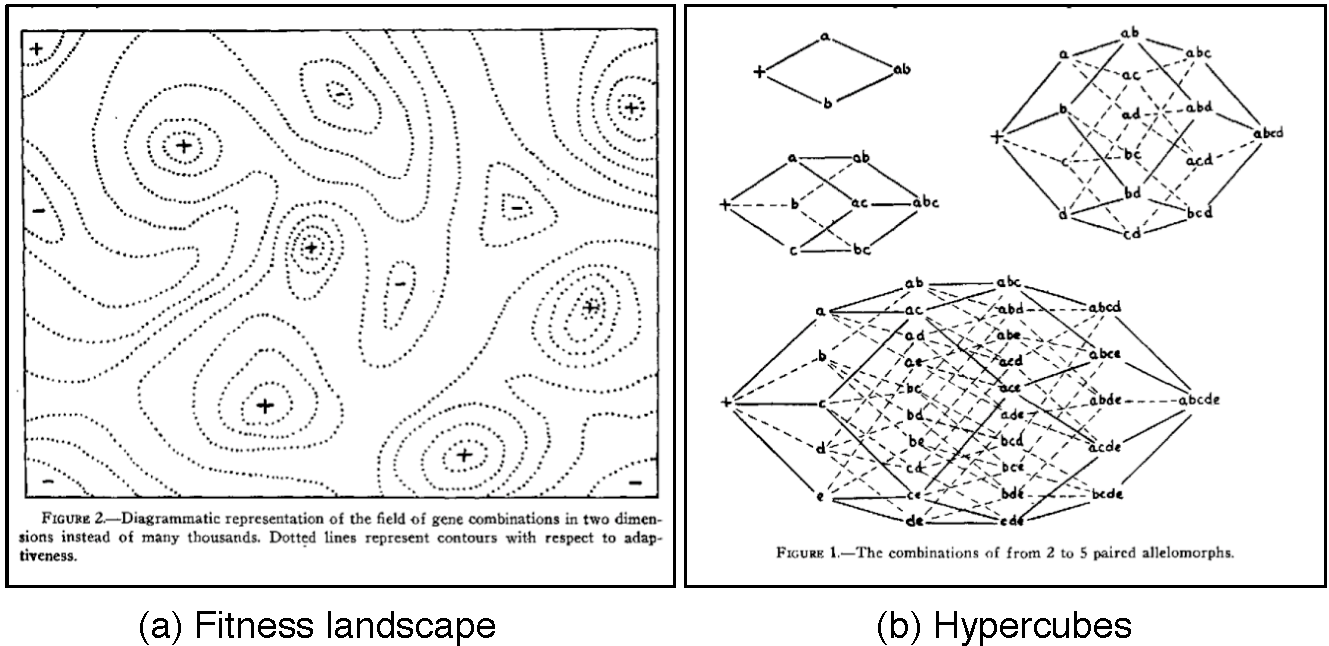
\includegraphics[width=0.9\columnwidth]{wrightland}}
\caption{\textbf{Wright's high dimensional genotypic representation.}
\small{Adapted from \citet{wright:1932aa} 
Panel (a) shows a simplified two dimensional space of ``allelomorphs".
The contours represent the scale of the adaptive value.
The second panel (b) shows the actual high dimensional genotypic `hypercubes'.
Each of the nodes are the different alleles or as Wright called them, `allelomorphs'.}
}
\label{wrightland}
\end{center}
\end{figure}
%

\textbf{Maynard Smith's Sequence Space.}\index{fitness!sequence space}\index{fitness!mutational landscape}
In the $\oldstylenums{1960}$'s John Maynard Smith developed a similar concept of sequence space but this time in the context of proteins \citep{maynard-smith:1970aa}.\index{Maynard Smith, John}
The protein code alphabet consists of the twenty amino acids.
For a protein chain of length $L$ there are $20^L$ possible combinations.
Each of these combinations can be represented in an $L$ dimensional space such that the sequences next to each other differ by just a single amino acid.
Maynard Smith concocted a recipe for finding adaptive walks in such high dimensional ``sequence space".
The dimensionality increases as the length of the sequence ($L$) increases.
For example for a three dimensional system we need to represent all the possible combinations in a three dimensional hypercube.
According to Maynard Smith, ``if evolution by natural selection is to occur, functional proteins (or DNA sequences) must form a continuous network which can be traversed by unit mutational steps without passing through non- functional intermediates" \citep{maynard-smith:1970aa}.
The landscape thus constructed is also known as ``mutational landscape" as the neighbours differ from each other by one mutational step.

\textbf{Eigen and Schuster's fusion of landscapes and fitness.}
Working together, Manfred Eigen and Peter Schuster \index{Eigen, Manfred}\index{Schuster, Peter} combined the concepts of sequence space and fitness.
If each sequence has its own fitness value and if we add this dimension to the already $L$ dimensional space then we get Wright's Adaptive landscape.
In this landscape all the $L$ dimensions are flattened out and we see a mountain range in the dimension of fitness.
This range can have peaks and valleys corresponding to the sequences with higher or lower fitnesses.
This landscape has been studied in detail by John Gillespie \citep{gillespie:1983aa,gillespie:1984aa}.
He was influential in utilizing the strong selection weak mutation (SSWM) assumption in staunch opposition of the neutral theory of Motoo Kimura \citep{gillespie:1984ab}.

Together these adaptive landscape models \citep{kauffman:1987aa} are able to capture the general properties of adaptive evolution as has been seen from experimental studies \citep{betancourt:2006ml}.
Let us review the commonalities between all these visualisations,
\begin{enumerate}[\textbf{--}]

\item For Fisher it was some trait combination which affected fitness and for Wright it was the genetic makeup which affected fitness.
For Maynard Smith it was the different mutational states of a sequence.
In all cases, the process involves identifying the variable which affects fitness.

\item Fisher used a sphere to demonstrate the idea of the geometrical model for three variables.
Wright used only two variables to illustrate an adaptive landscape Fig.\ \ref{wrightland}\ (a).
Although these are for illustrative purposes both of them knew that actually the effective number of variables are many and thus the resulting variable space is high dimensional Fig.\ \ref{wrightland}\ (b).
As noted in \citep{kauffman:1989aa}, \textit{``$\ldots$the concept is very general, and can be used to represent entire organisms or other ensembles of related objects that are "one mutant neighbors" of each other."}

\item Fitness adds another dimension to this already high dimensional trait space.
This is the dimension which actually gives a shape to the otherwise featureless trait space.

\item Change is a major constant in biology.
One major assumption with these models was that the fitness landscape remains unchanged.
For example Wright constructed the concept of an adaptive landscape assuming that the genotypic fitnesses remain constant over time \citep{provine:1986bo}.
As the populations moves over the fitness landscape, if the fitness is frequency dependent, then the shape of the landscape will change.
The earliest reference to frequency dependent selection is given by \citet{poulton:1884aa} about the way predators maintain the colour polymorphism in their prey.
The explanation of one of the most puzzling of puzzles in biology, evolution and maintenance of sex, is hypothesised to be change.
The Vicar of Bray hypothesis suggests that sex helps produce a variability in the phenotypes of the offspring, some of which may be better suited to a change in the ecology of the environment \citep{ridley:2003bo}.\index{frequency dependence!Vicar of Bray Hypothesis}
The Red Queen hypothesis tackles the question at a different level \citep{vanVaalen:1973aa}.\index{frequency dependence!Red Queen Hypothesis}
Sex and the evolutionary existence of males are explained by their ability to preserve the genes which can provide an evolutionary advantage against a changing ecology.
Frequency dependent fitness effects have been documented in a number of experimental tests carried out in \textit{Drosophila} \citep{ayala:1974aa,hartl:1997bo} and are proposed to be one of the mechanisms maintaining a high degree of polymorphism for example in the Major Histocompatibility Complex (MHC) \citep{borghans:2004oe,milinski:2006mh}.
Frequency dependence is also a crucial factor when addressing the question of biodiversity \citep{levin:2000aa}.\index{frequency dependence}
\end{enumerate}

The scope of this thesis is limited to exploring two main themes of these approaches,
\begin{enumerate}[\textbf{--}]
\item Higher dimensions in static fitness landscapes.
\item Higher dimensions in frequency dependent fitness landscapes.
\end{enumerate}

The organisation of these two issues in this thesis is explained in the next section (see Fig.\ \ref{fig:outline1}).

\section{Thesis Overview}

Fisher, Wright and Maynard Smith thought about specific variables affecting fitness.
We abstract it further to another level where we just consider them as some variables affecting fitness.
In a cultural sense these could be behavioural traits, fads or fashion or on the genetic level they could be particular alleles of a gene, genes, genetic regulatory networks etc.\ .
Hence thinking on a further abstract level we free ourselves from the conditions of the dimensions being genotypically or phenotypically determined.
They could be any characteristics which in a certain combination affect fitness.
%
\begin{figure}[!h]
\begin{center}
\leavevmode
\boxed{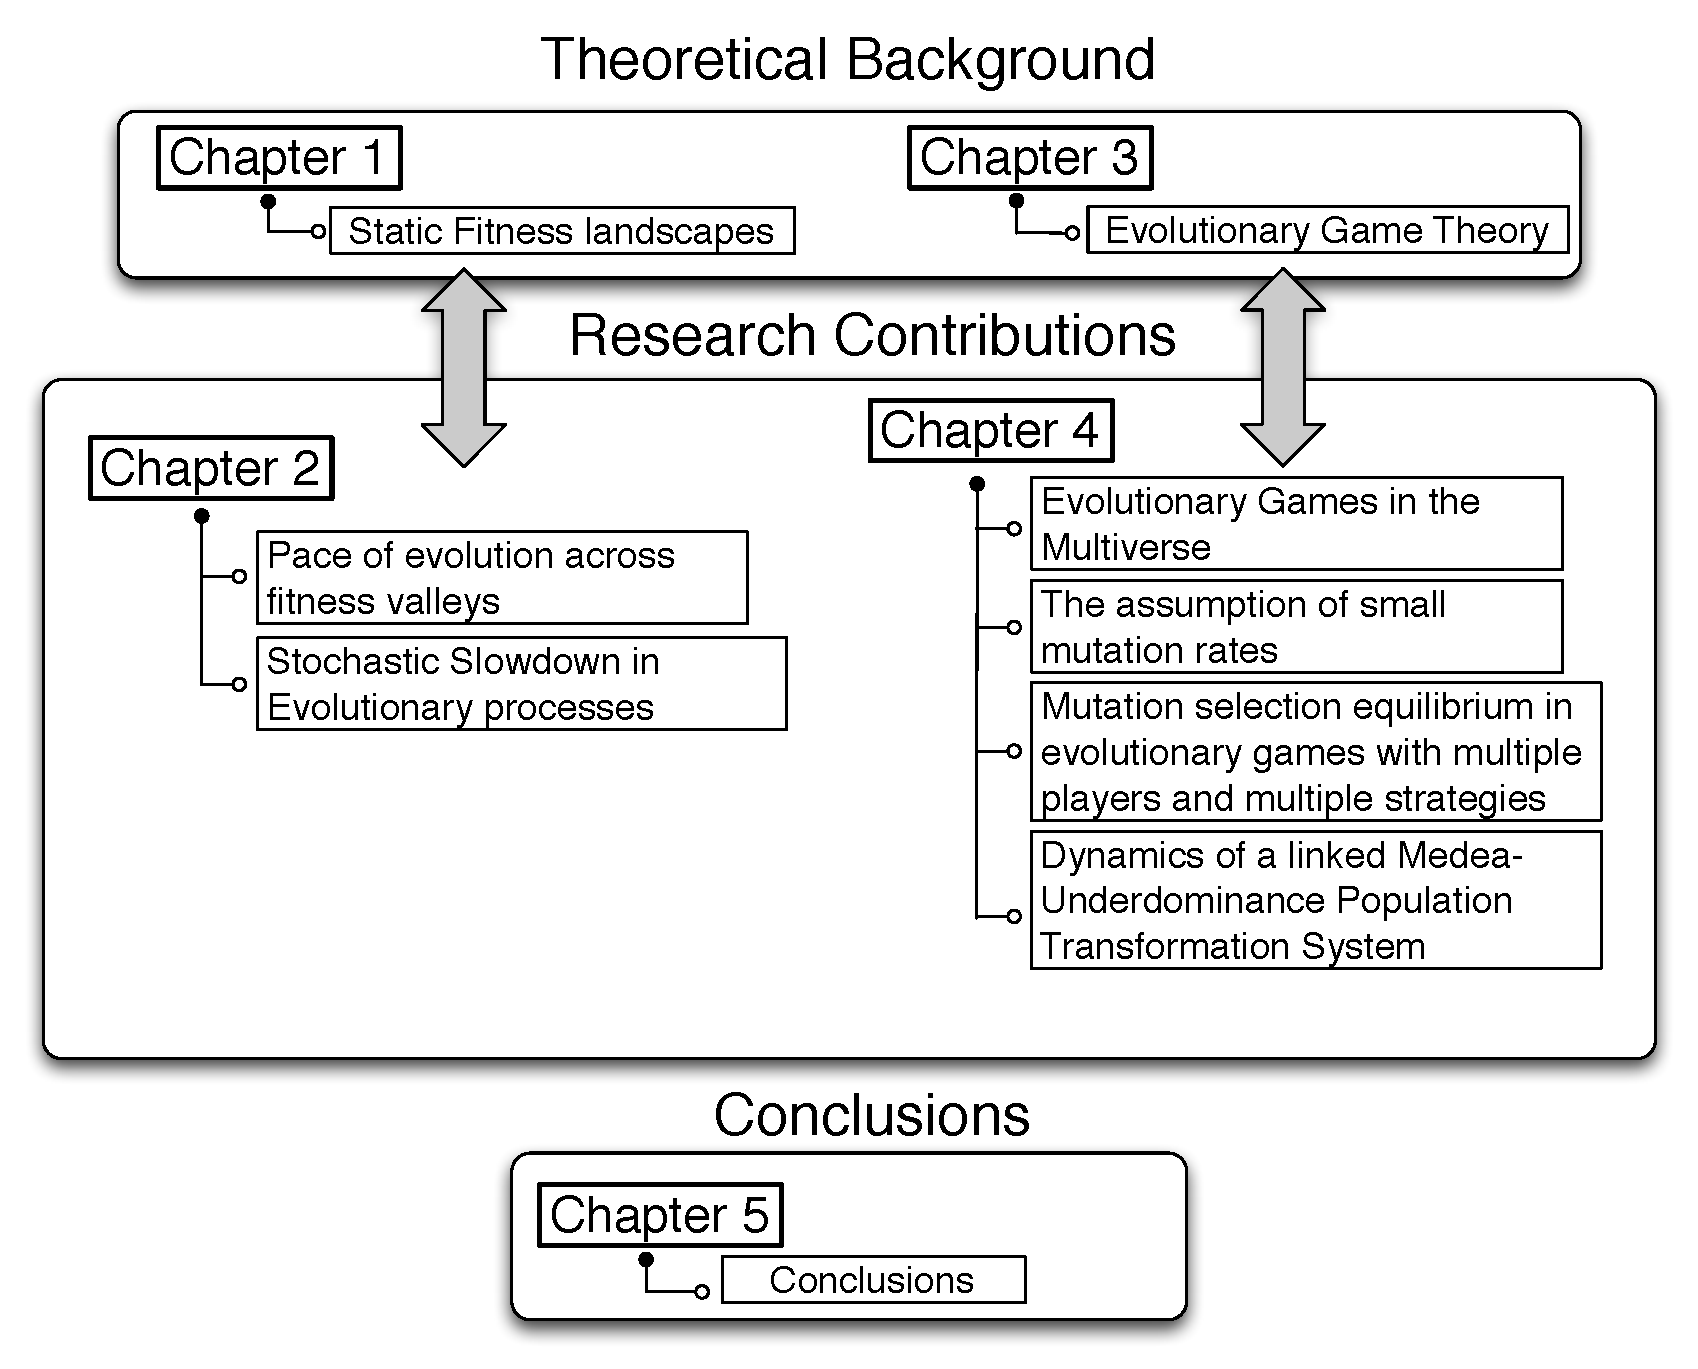
\includegraphics[scale=0.40]{outline1}}
\caption{\textbf{Outline of the thesis.}
\small{The thesis layout follows the flow of ideas rather than the chronology of publications.
Chapter \ref{chap:intro} provides a general background of evolutionary theory and an introduction to static fitness landscapes.
Chapter \ref{chap:speed} directly follows from the theory of static landscapes.
We then move on to the theoretical background of dynamic fitness landscapes and in particular the use of evolutionary game theory in Chapter \ref{chap:egttheory}. Chapter \ref{chap:multiverse} includes the publications relating to evolutionary game theory and the Chapter \ref{chap:conclu} collates all the results together and concludes the thesis with final remarks.}
}
\label{fig:outline1}
\end{center}
\end{figure}
%

\noindent
Chapter \ref{chap:speed} is devoted to the question of the speed of adaptation on static landscapes.
In it two publications are documented,
%
\begin{enumerate}[2.1]

\item \textbf{Chaitanya S. Gokhale}, Yoh Iwasa, Martin A. Nowak, Arne Traulsen,\\
  	The pace of evolution across fitness valleys,\\
	\textit{Journal of Theoretical Biology}, \textbf{259}, (2009)\\
	Page \pageref{sec:fitval}

\item Philipp M. Altrock, \textbf{Chaitanya S. Gokhale}, Arne Traulsen\\
  	Stochastic slowdown in evolutionary processes,\\
	\textit{Physical Review E}, \textbf{82, 011925}, (2010)\\
	Page \pageref{sec:stoslo}

\end{enumerate}
%

\noindent
Chapter \ref{chap:egttheory} is an introduction to evolutionary game theory.
We move from our discussion of static fitness landscapes to frequency dependent fitness landscapes.
For addressing this issue we rely on evolutionary game theory as a tool to study the evolutionary dynamics.
In this chapter the basic concepts of evolutionary game theory pertaining to the scope of this thesis are introduced.

\noindent
Chapter \ref{chap:multiverse} is an extension of the theory discussed in Chapter \ref{chap:egttheory}.
It consists of four publications.
The  first three are theoretical advancements while the fourth is an evolutionary game theoretic analysis of an experimental setup.

\begin{enumerate}[4.1]
\item \textbf{Chaitanya S. Gokhale}, Arne Traulsen,\\
  	Evolutionary games in the multiverse,\\
	\textit{Proceedings of the National Academy of Sciences, USA}, \textbf{107}, (2010)\\
	Page \pageref{chap:multiverse}
	
\item Bin Wu, \textbf{Chaitanya S. Gokhale}, Long Wang, Arne Traulsen,\\
  	How small are small mutation rates?,\\
	\textit{Journal of Mathematical Biology, In revision}\\
	Page \pageref{sec:wgt}
	
\item \textbf{Chaitanya S. Gokhale}, Arne Traulsen,\\
	Mutation-selection equilibrium in evolutionary games with multiple players and multiple strategies,\\
	\textit{Submitted}\\
	Page \pageref{sec:equilibrium}

\item \textbf{Chaitanya S. Gokhale}, R. Guy Reeves, Floyd A. Reed,\\
  	Dynamics of a linked Medea-Underdominance Population Transformation System\\
	\textit{In preparation}\\
	Page \pageref{chap:medea}
\end{enumerate}

\noindent
Detailed author contributions are reviewed at the end of the thesis in Table \ref{tab:contributions}.

%---------------------------------------------Pace of evolution-------------------------------------------------


\begin{savequote}[13pc]
\sffamily
``Life is a high-country adventure"
\qauthor{Stuart Kauffman}
\end{savequote}

\chapter{Speed of evolution}
\label{chap:speed}

\section{Pace of evolution across fitness valleys}
\graphicspath{{Figs_Pace/}{Figs_Pace/}{Figs_Pace/}}

\label{sec:fitval}

\textit{``The problem of evolution as I see it is that of a mechanism by which the species may continually find its way from lower to higher peaks [$\ldots$].
In order that this may occur, there must be some trial and error mechanism on a grand scale [$\ldots$].
To evolve, the species must not be under strict natural selection.
Is there such a trial and error mechanism?"}
\citep{wright:1932aa}.

Wright had asked a very interesting question in theoretical population dynamics.
How a population which is stuck at one of the many possible local fitness maxima evolve to the global fitness maximum.
Fisher, who thought in a much more geometrical way, envisioned that any local fitness maxima would be a point on the slope of another adaptive hill in a higher dimension.
Thus given enough time, a population would finally make it to the global maximum.
Wright was more in favour of random drift.
He believed that by drift populations could reach the foots of other hills and then selection could take over so as to drive the populations uphill towards the peak.
In his \textit{Shifting Balance Theory}, Wright postulates that a number of sub-populations could explore the fitness landscapes and as the number of sub-populations increases, the chance that one of them finds the global optimum also increases \citep{wright:1932aa}.\index{Wright, Sewall!Shifting Balance theory}
Once at the global optimum, that sub-population will outcompete all the other types of that species and the species as a whole will have reached the global adaptive peak \citep{ridley:1996bo}.

We address the question using the mutational landscape.
Mutations during individual reproduction are either ultimately lost (when the mutants go extinct) or
fixed in a population (when the mutants take over). The probability that a mutation reaches fixation 
increases with the relative fitness of the mutant. 
As the fitness landscape is made up of mutants which are one mutational step away from each other, we can ask the question how long it takes until a number of mutations reach fixation. 
Of course, this depends on the fitness of the mutants. 
But in addition, the order of mutations is crucial: 
%
\begin{enumerate}
\item If each mutation needs another mutation as a prerequisite to occur, 
evolution occurs on a single path or ridge in fitness landscape. 
\item If the order of mutations is arbitrary, then there are many paths possible along which the mutations are
accumulating and evolution typically proceeds faster. 
\end{enumerate}
%
\begin{figure}[h]
  \begin{center}
      \boxed{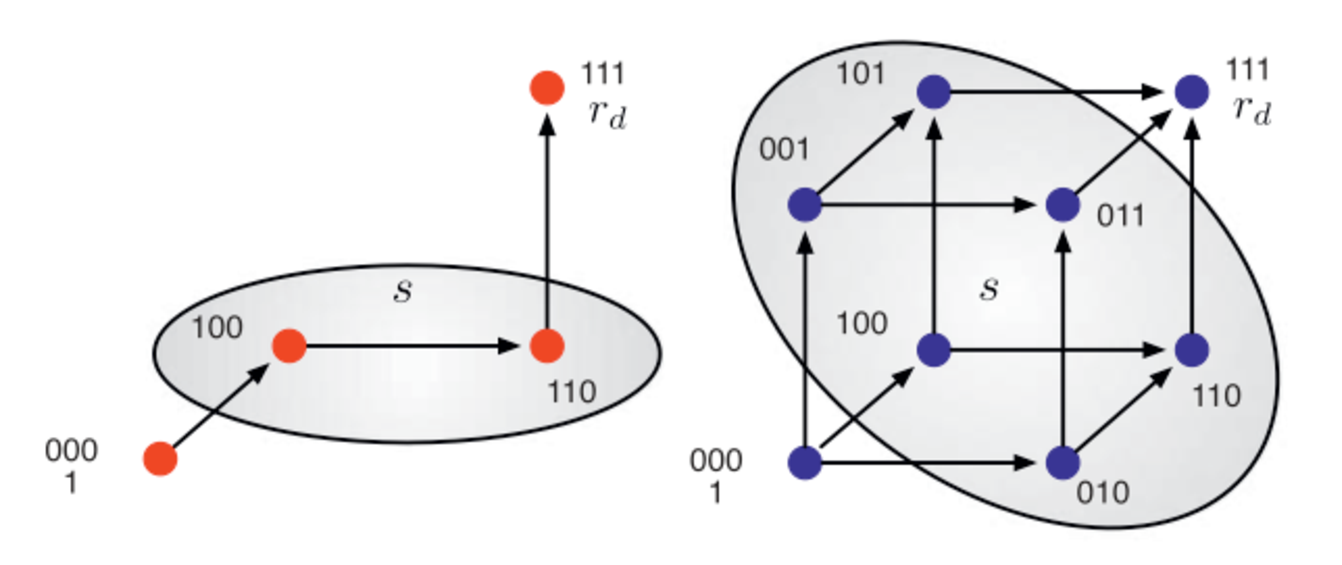
\includegraphics[width=0.8\columnwidth]{paperfig}}
    \caption{\textbf{Single path and Hypercube.}
    \small{Hypothetical fitness paths where only a fixed sequence of mutation can lead to the state of higher fitness (single path) or a multitude of paths lead to the ultimate state (hypercube).
The intermediate states are all assumed to have the same fitness $s$ as compared to the fitness of the initial state considered to be $1$ and the final state as $r_d$.}
}
    \label{fig:paperfig}
  \end{center}
\end{figure}
%
We address the pace of evolution in the two scenarios (see Fig.\ \ref{fig:paperfig}) and show how the size of the population affects the way a population evolves. 
The developed theory allows us to ask when evolution occurs faster on a narrow ridge or through a broad valley with disadvantageous intermediate mutations.

The framework developed here can serve as a reference case for evolution in real fitness landscapes, 
as it can be easily extended to incorporate the complexity and variation seen in experimental studies, Fig.\ \ref{fig:expfitland}.
%
\begin{figure}[h]
  \begin{center}
      \boxed{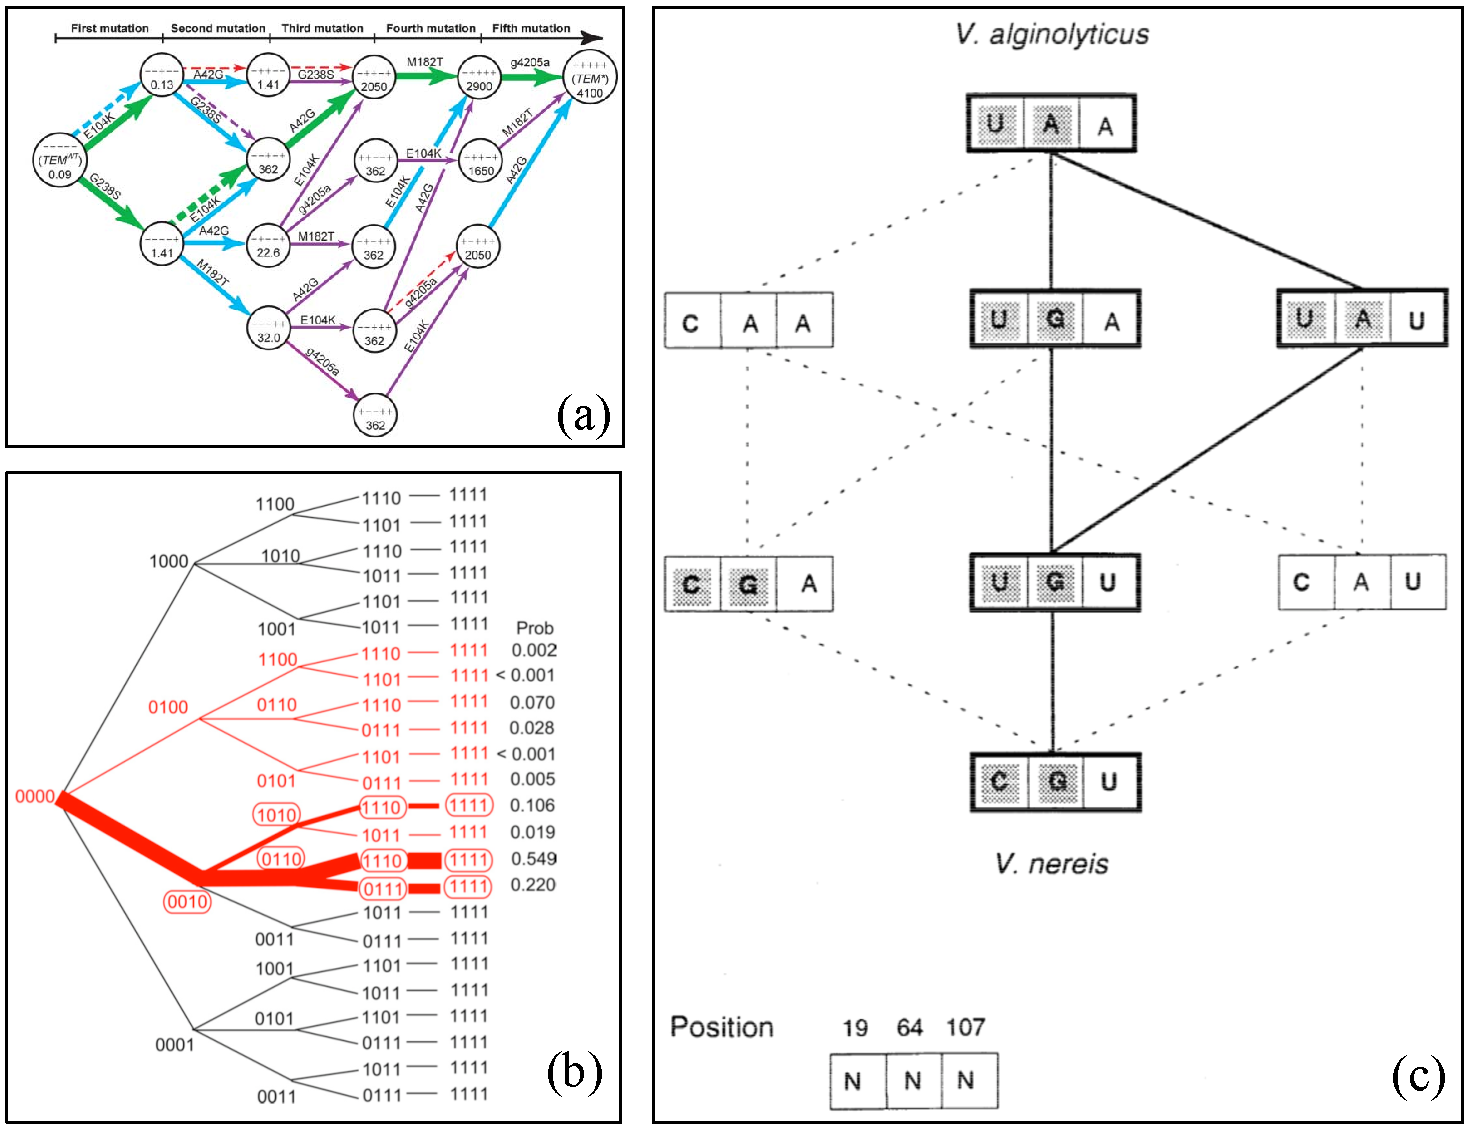
\includegraphics[width=0.9\columnwidth]{experimentpaths}}
    \caption{\textbf{Examples of experimentally constructed fitness landscapes.}
\small{The images collated from:
    (a) \citet{weinreich:2006aa}: Mutational paths in the $\beta$ lactamase gene conferring resistance to bacteria from $\beta$ lactam antibiotics where were found to be viable.(b) \citet{lozovsky:2009aa}: The major inferred pathways for the evolution of pyrimethamine resistance. (c) \citet{lee:1997}: All paths between the 5srRNA sequences of \textit{Vibrio proteolyticus} and \textit{V. nereis} at the three positions where they differ.}
    }
    \label{fig:expfitland}
  \end{center}
\end{figure}
%
\index{$beta$ lactamase}
\index{$beta$ lactamase!$beta$ lactam antibiotics}
\index{\textit{Vibrio}!\textit{Vibrio proteolyticus}}
\index{\textit{Vibrio}!\textit{Vibrio nereis}}
This way of approaching the problem lets us explore the different regimes of mutation rate.
%
\begin{figure}[h]
  \begin{center}
      \boxed{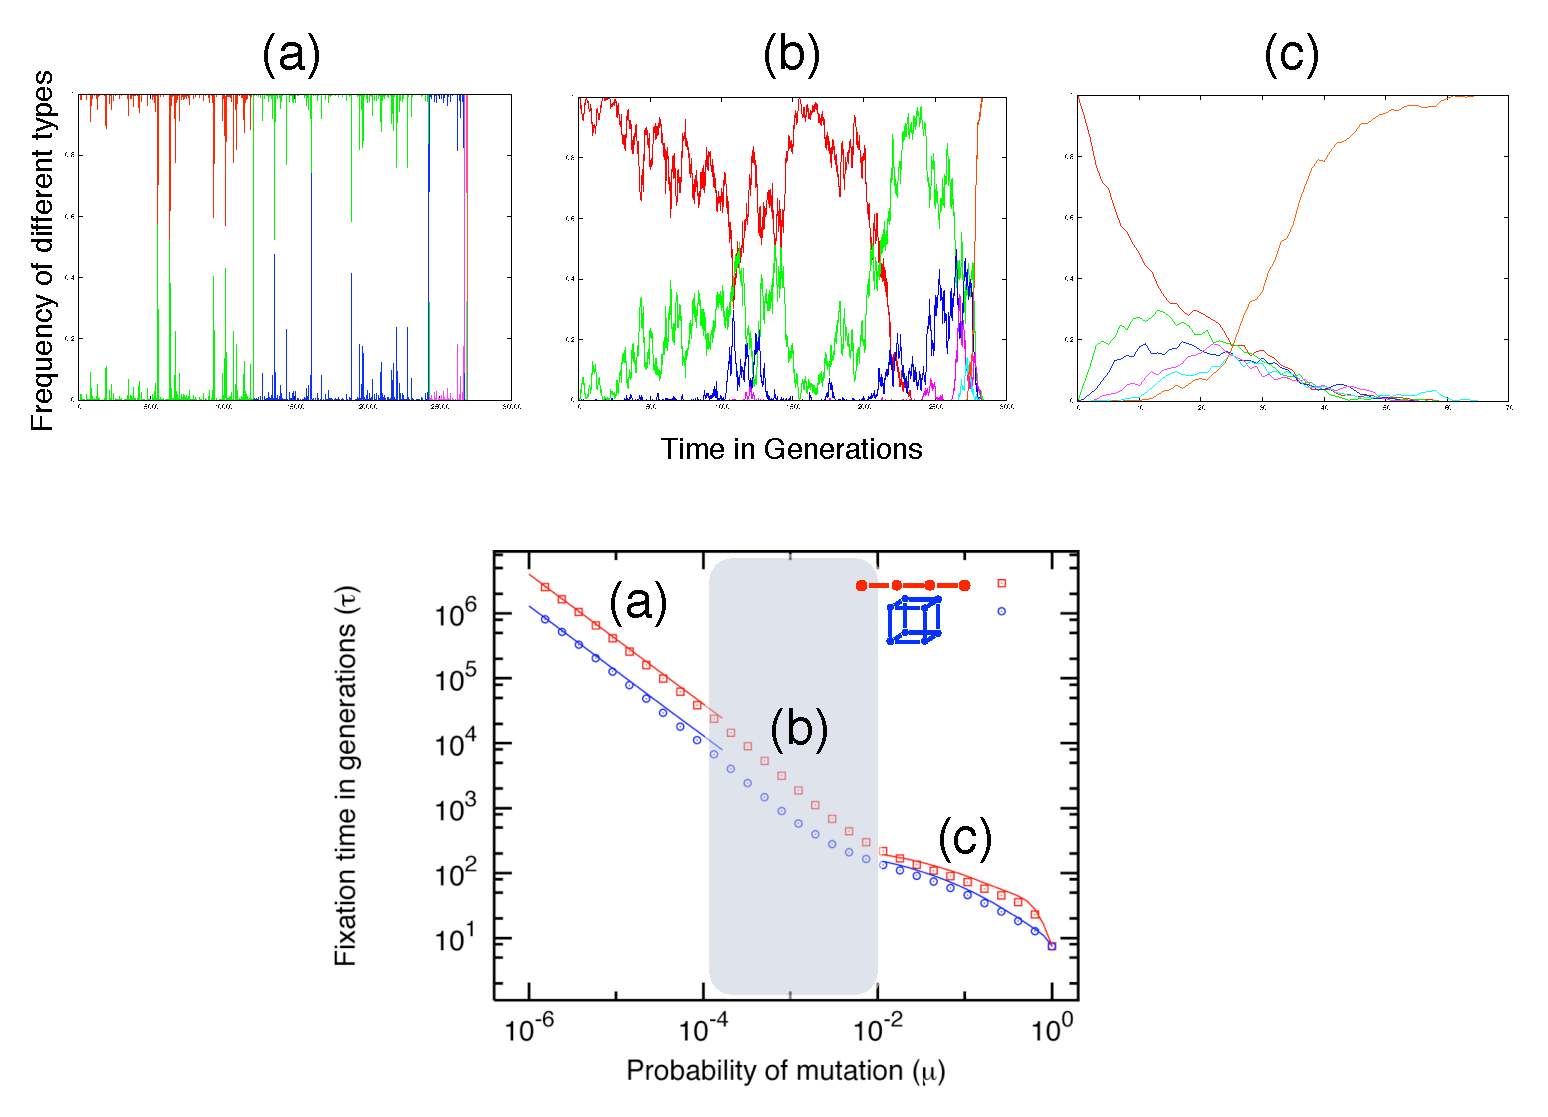
\includegraphics[width=0.8\columnwidth]{mutationspectrum}}
    \caption{\textbf{Regimes of mutation rates.}
\small{(a) If mutation rates are very low then the system is monomorphic most of the time, occasionally a mutation occurs and it can either go extinct or reach fixation.
This scenario can be captured analytically. (b) For intermediate mutation rates multiple mutants can coexist and the situation is difficult to characterise analytically.
(c) For high mutation rates the dynamics can be approximated by differential equations again yielding tractable results.}
}
    \label{mutspectrum}
  \end{center}
\end{figure}
%
\begin{itemize}

\item For \textbf{small mutation rates} the population evolves by a process where the mutations occur one 
after the other, which has been termed periodic selection \citep{atwood:1951aa} and theoretically described as the strong-selection 
weak-mutation regime \citep{gillespie:1983aa,gillespie:2004bo} (see Fig.\ \ref{mutspectrum} (a)).
\index{periodic selection}
\item For \textbf{intermediate mutation rates} the population does not move from mutational step to the next as a whole.
Instead many mutants are present in the population at the same time.
This phenomenon of competition amongst multiple mutants termed as clonal interference or stochastic tunneling has been a subject of in-depth theoretical and experimental studies. \citep{gerrish:1998aa,elena:1998aa,elena:2003aa,iwasa:2004aa,park:2007aa}.
This process is of importance in studies related to cancer initiation \citep{iwasa:2004aa,michor:2004aa,beerenwinkel:2007aa,beerenwinkel:2007qy,bozic:2010aa} (see Fig.\ \ref{mutspectrum} (b)).
\index{clonal interference}\index{stochastic tunneling}
\item For \textbf{high mutation rates} the system we can use ordinary differential equations to capture the behavior of the system (see Fig.\ \ref{mutspectrum} (c)).

\end{itemize}

This approach has been used to investigate how different strains of pathogens can evolve from one another \citep{alexander:2010td} or how long does it take for a population to acquire complex adaptive traits \citep{lynch:2010aa,lynch:2010ab}.

\subsection{Publication: The pace of evolution across fitness valleys}

Chaitanya S. Gokhale, Yoh Iwasa, Martin A. Nowak, Arne Traulsen,\\
Journal of Theoretical Biology\\
$2010$\\
Volume $259$\\
Pages $613-620$
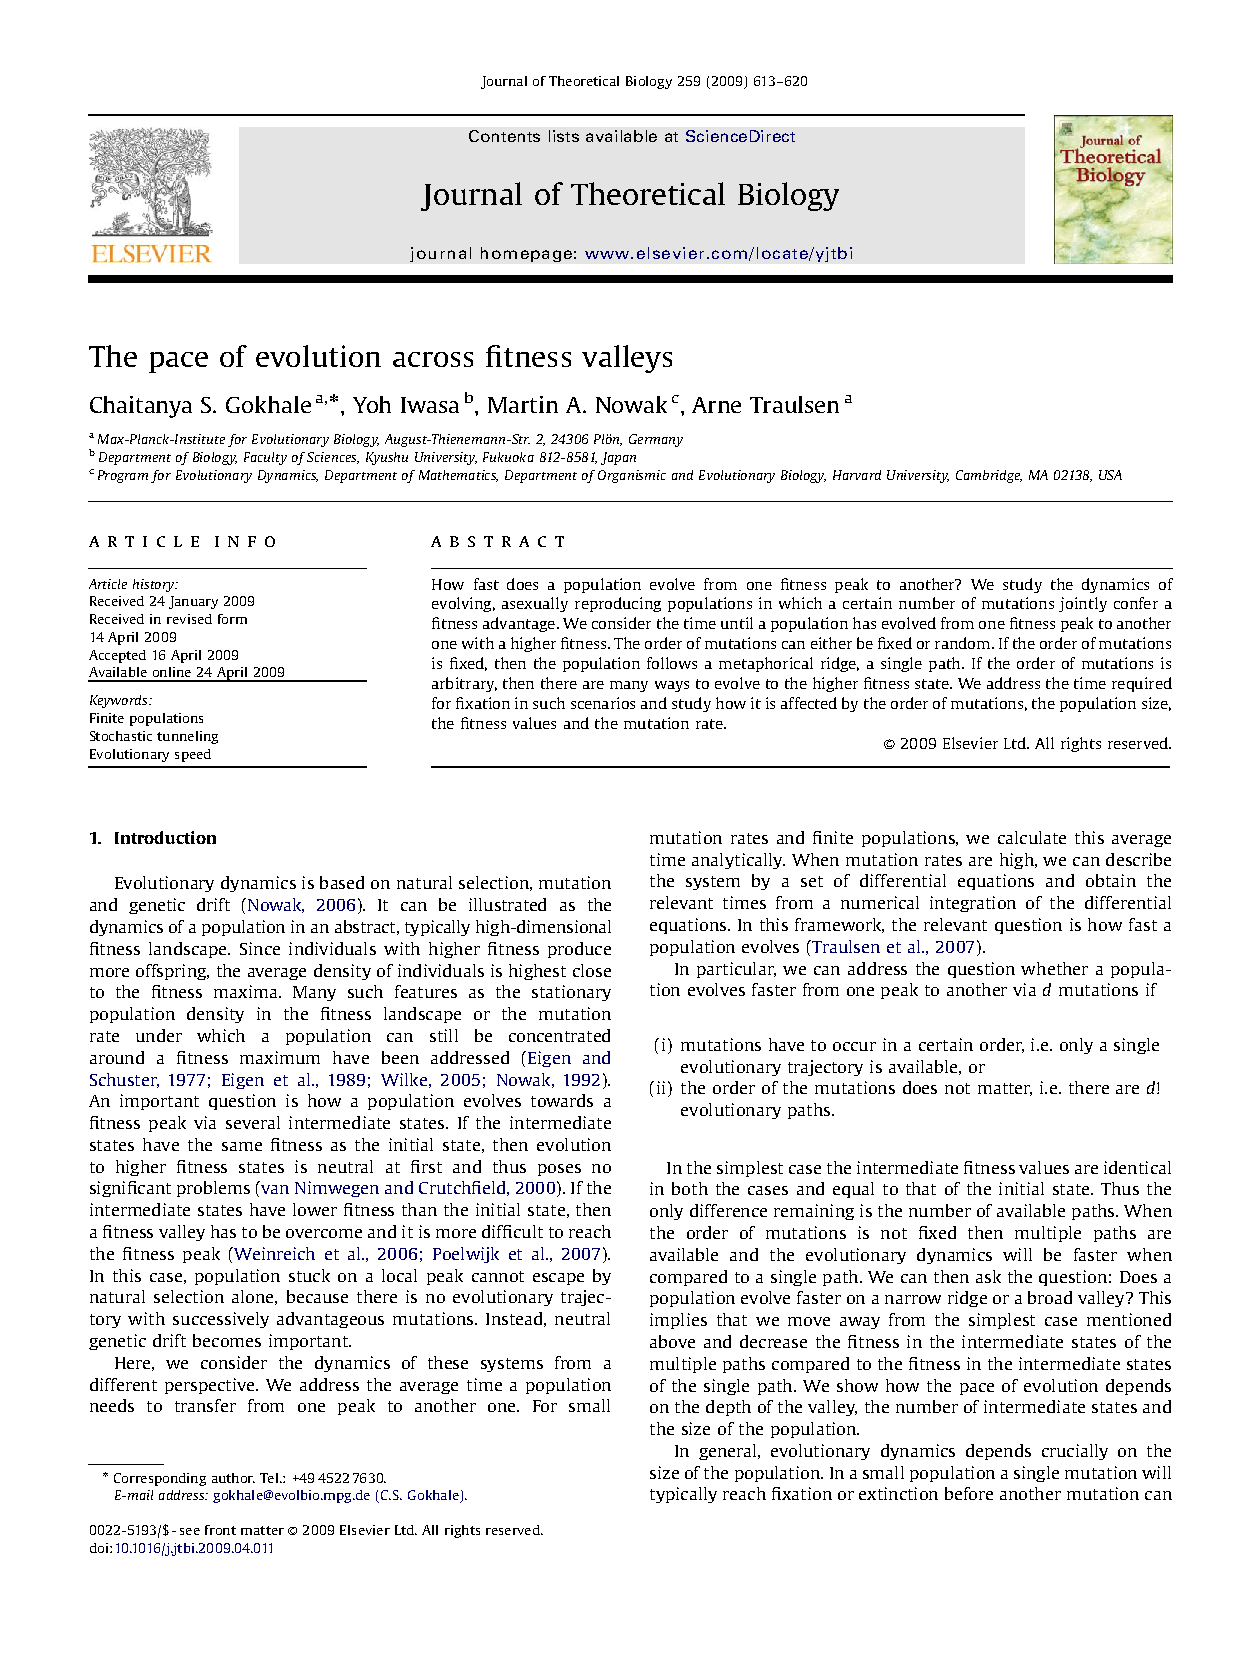
\includepdf[pages=-,scale=0.8]{Papers/Gokhale_JTB_2009.pdf}

%---------------------------------------------Stochastic Slowdown-------------------------------------------------

\section{Fitter but slower}
\label{sec:stoslo}
\graphicspath{{Figs_Stoslo/}{Figs_Stoslo/}{Figs_Stoslo/}}

During the earlier study an interesting counterintuitive characteristic was noted.
Consider the following simple setup.
There are only two states $A$ and $B$.
The whole population (of size $N$) currently resides in state $B$.
An individual can move from state $B$ to state $A$ by acquiring a mutation but not vice versa.
%
\index{stochastic processes!Wright-Fisher process}
\index{stochastic processes!Moran process}
\begin{figure}[!h]
  \begin{center}
    \boxed{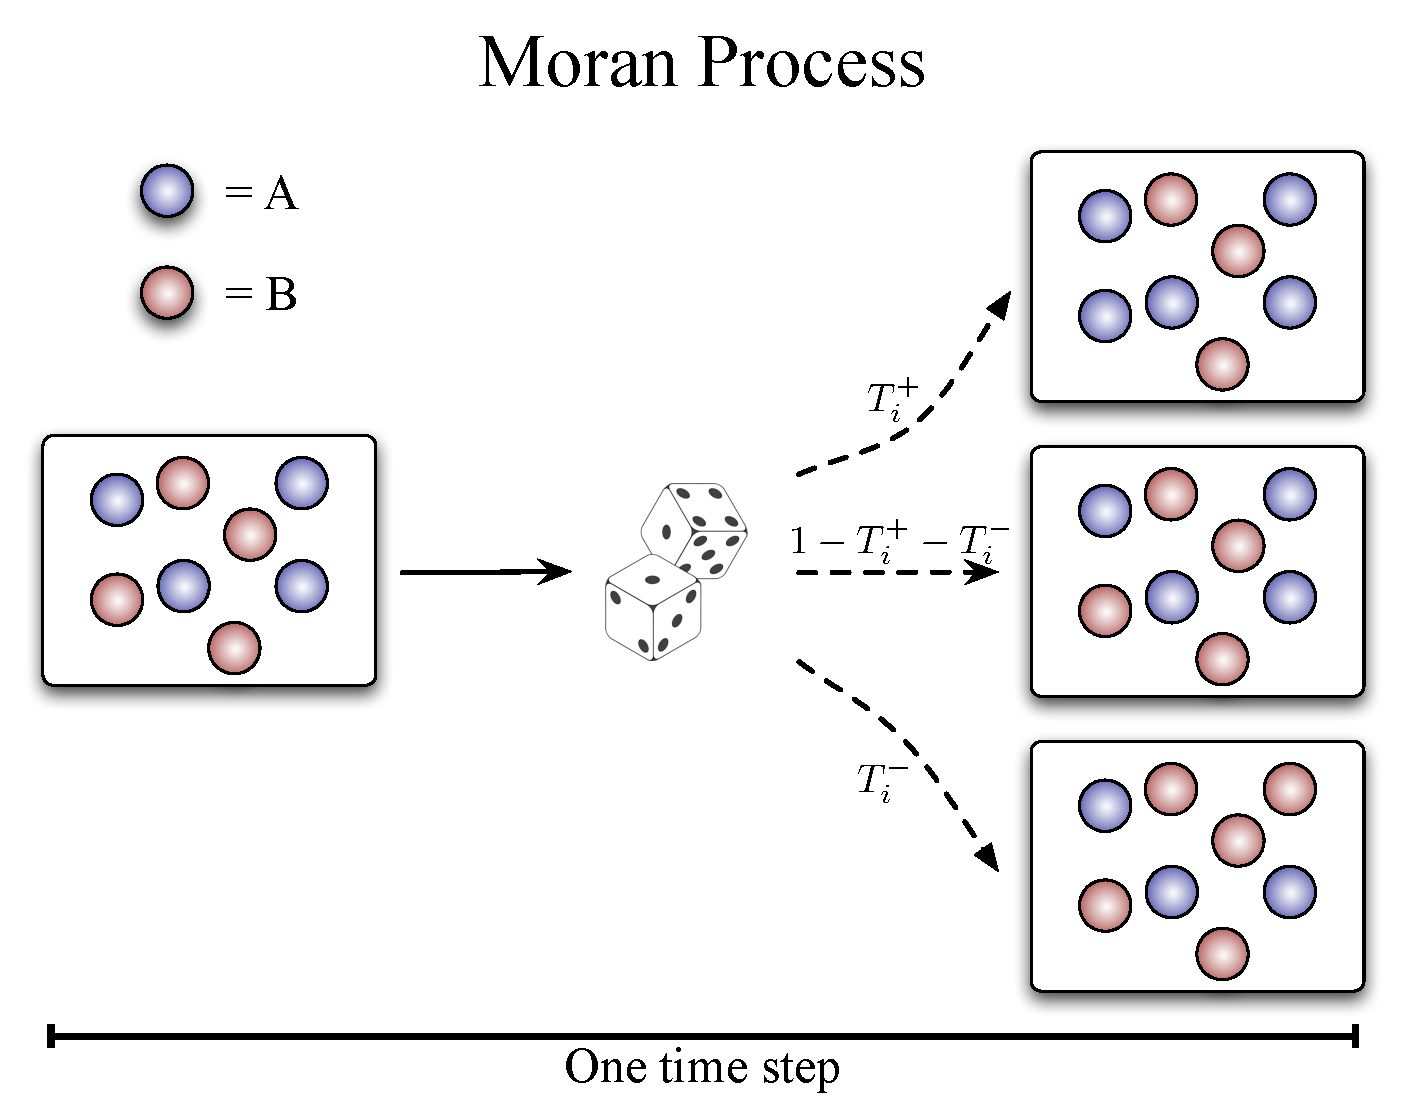
\includegraphics[width=0.7\columnwidth]{moranprocess}}
  \end{center}
  \caption{
  \label{fig:moran}
  \textbf{The Moran process.}
\small{ To describe the dynamics of a population of finite size we resort to stochastic processes.
 The Moran process is a birth-death process. 
 That is, in time each step a birth event and a death event occur.
 The population size is maintained constant by a random death.
 If the population consists of say $i$ $A$ individuals then in one time step the number of $A$ can increase by one (with probability $T_i^+$) or decrease by one (with probability $T_i^-$) or stay the same (with probability $1-T_i^+ -T_i^-$).}
  }
\end{figure}
%
For the dynamics we make use of the Moran process \citep{moran:1962ef}.
Each time step of the Moran process consists of a birth even and a death event.
For the whole population to move from state $B$ to state $A$ means that all individuals currently in state $B$ have to acquire the mutation.
The mutation rate is given by $\mu$.
We consider the limit of small mutation rates such that a mutant reaches its fate (either fixation or extinction) before a new one arises.
There are no back mutations from $A$ to $B$.
Thus in our variant of the Moran process in each time step, one of the following three things can happen (see Fig.\ \ref{fig:moran}),\index{stochastic processes!transition probabilities}
%
\begin{itemize}
\item \textbf{Number of individuals in state $\mathbf{A}$ increases by 1.}
The number of individuals in state $A$ increases by $1$ with probability,
%
\begin{equation}
T_i^+ = \frac{i}{N} \frac{N-i}{N} + \frac{N-i}{N} \mu \frac{N-i}{N}.
\end{equation}
%
The increase can happen in two ways.
The first term gives the probability when an $A$ state individual is chosen for reproduction and a $B$ for death.
The second term gives the probability when a $B$ is chosen for reproduction, but mutates to $A$ and again a $B$ is chosen for death.

\item \textbf{Number of individuals in state $\mathbf{A}$ decreases by 1.}
The number in state $A$ decreases only if a $B$ is chosen for reproduction and it does not mutate and an $A$ is chosen for death.
This event happens with probability,
%
\begin{equation}
T_i^- = \frac{N-i}{N} (1-\mu) \frac{i}{N}.
\end{equation}
%
\item \textbf{No change in either state.}
This happens with probability $1-T_i^+ - T_i^-$.
\end{itemize}
%

Hence in each reproductive step there is a bias towards producing an individual with a mutation (see Fig.\ \ref{fig:stoslo}).
%
\begin{figure}[h]
  \begin{center}
      \boxed{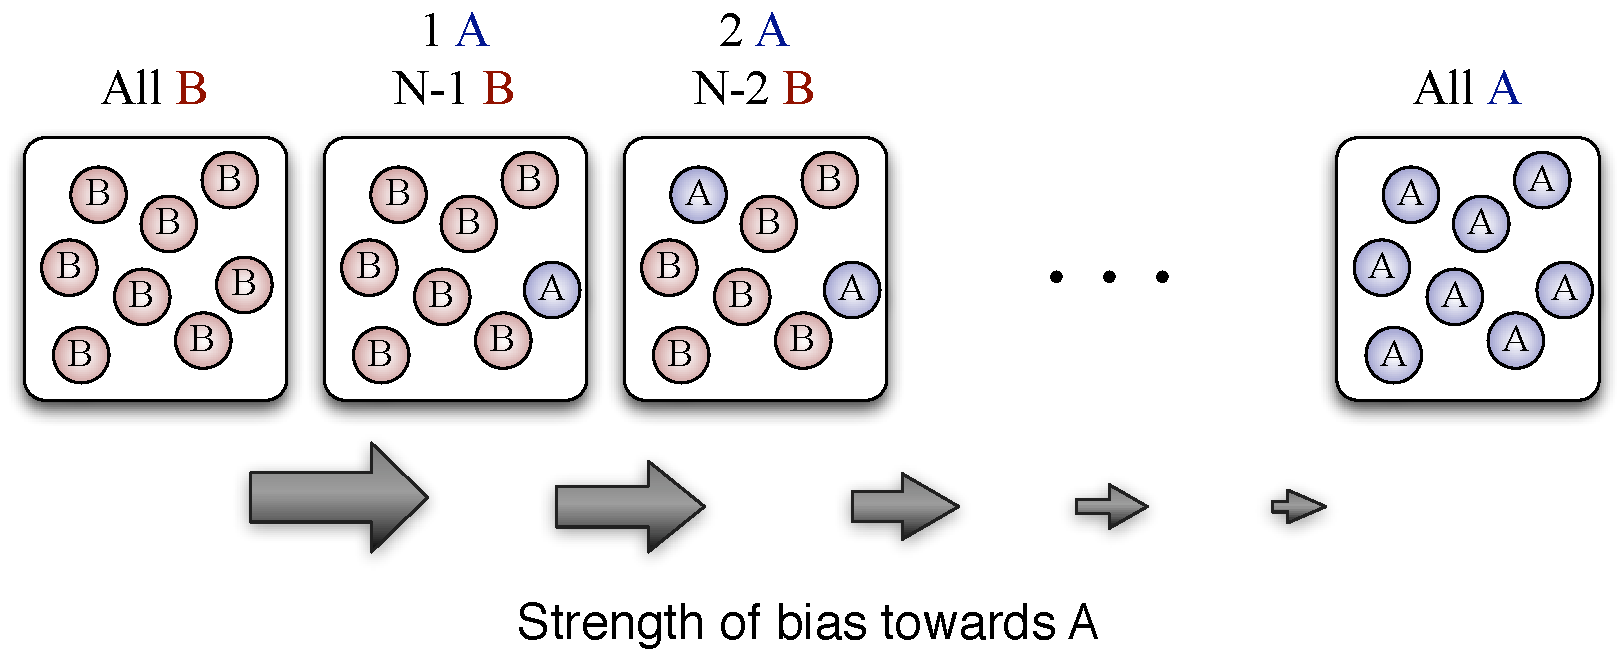
\includegraphics[width=0.9\columnwidth]{stoslooutline}}
    \caption{\textbf{Bias towards $A$.}
\small{Throughout the process there is a frequency dependent bias towards moving to an all $A$ state.
It diminishes in strength as the system gets closer to an all $A$ state.
    Yet the time time required to get to the final state is greater than without such a bias.}
}
    \label{fig:stoslo}
  \end{center}
\end{figure}
%
Intuitively we expect that the average conditional time required for the fixation of a single $A$ individual in a population of $N-1$ $B$ individuals should be smaller than in a balanced process in which there is no bias.
However, we observe that for a small bias the average conditional fixation time is larger than that of a balanced process (without bias).

%
\begin{figure}[!h]
  \begin{center}
      \boxed{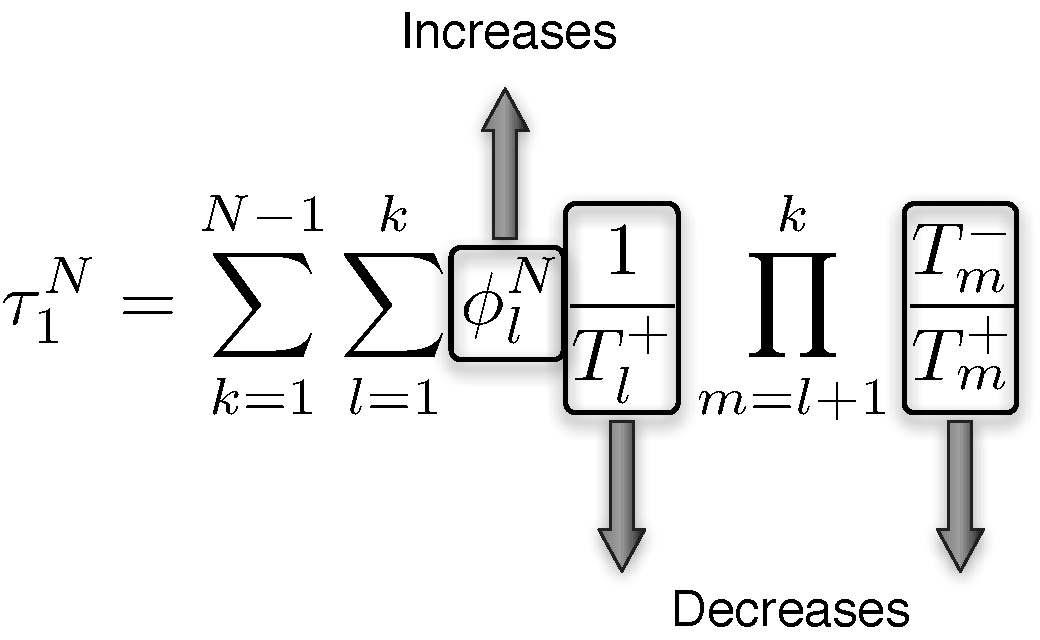
\includegraphics[width=0.4\columnwidth]{stosloeffect}}
    \caption{\textbf{Effect of increasing bias on components of conditional fixation time $\mathbf{\tau_1^{N}}$.}
    \small{The expression gives us the exact conditional fixation time $\tau_1^{N}$ for the Moran process beginning with a single mutant.
    If we introduce a frequency dependent bias such that we have $T_i^+ > T_i^-$, then we see that the ratio of transition probabilities and the inverse of $T_l^+$ decrease.
    On the contrary, the fixation probability, $\phi_l^N$, increases.
    The effect of this tug of war is an increase in the conditional fixation time for a small bias.}
 }
    \label{fig:stosloeffect}
  \end{center}
\end{figure}
%

To go to the heart of this counterintuitive observation we must dissect out the quantity of interest, the conditional fixation time.
Conditional fixation time means given that the mutant does fix, what is the time required for the population to reach a state where all individuals are mutants.\index{stochastic processes!fixation time!conditional fixation time}
For the Moran process we can exactly calculate the conditional fixation time from a formula which is well known for such a birth-death process \citep{moran:1962ef,goel:1974aa,ewens:1979qe,landauer:1987pr,antal:2006aa,traulsen:2009bb} (see Fig.\ \ref{fig:stosloeffect}).
In the following publication we observe what happens to this quantity of interest as we introduce a small bias to the system.
Even a simpler process than directed mutations can exhibit such counter-intuitive behaviour.
All it requires is a slight asymmetry in the transition probabilities ($T_i^+$ and $T_i^-$).

\newpage
\subsection{Publication: Stochastic slowdown in evolutionary processes}

Philipp M. Altrock, Chaitanya S. Gokhale, Arne Traulsen\\
\textit{Physical Review E}\\
$2010$\\
Volume $82$\\
Pages $011925$-$7$
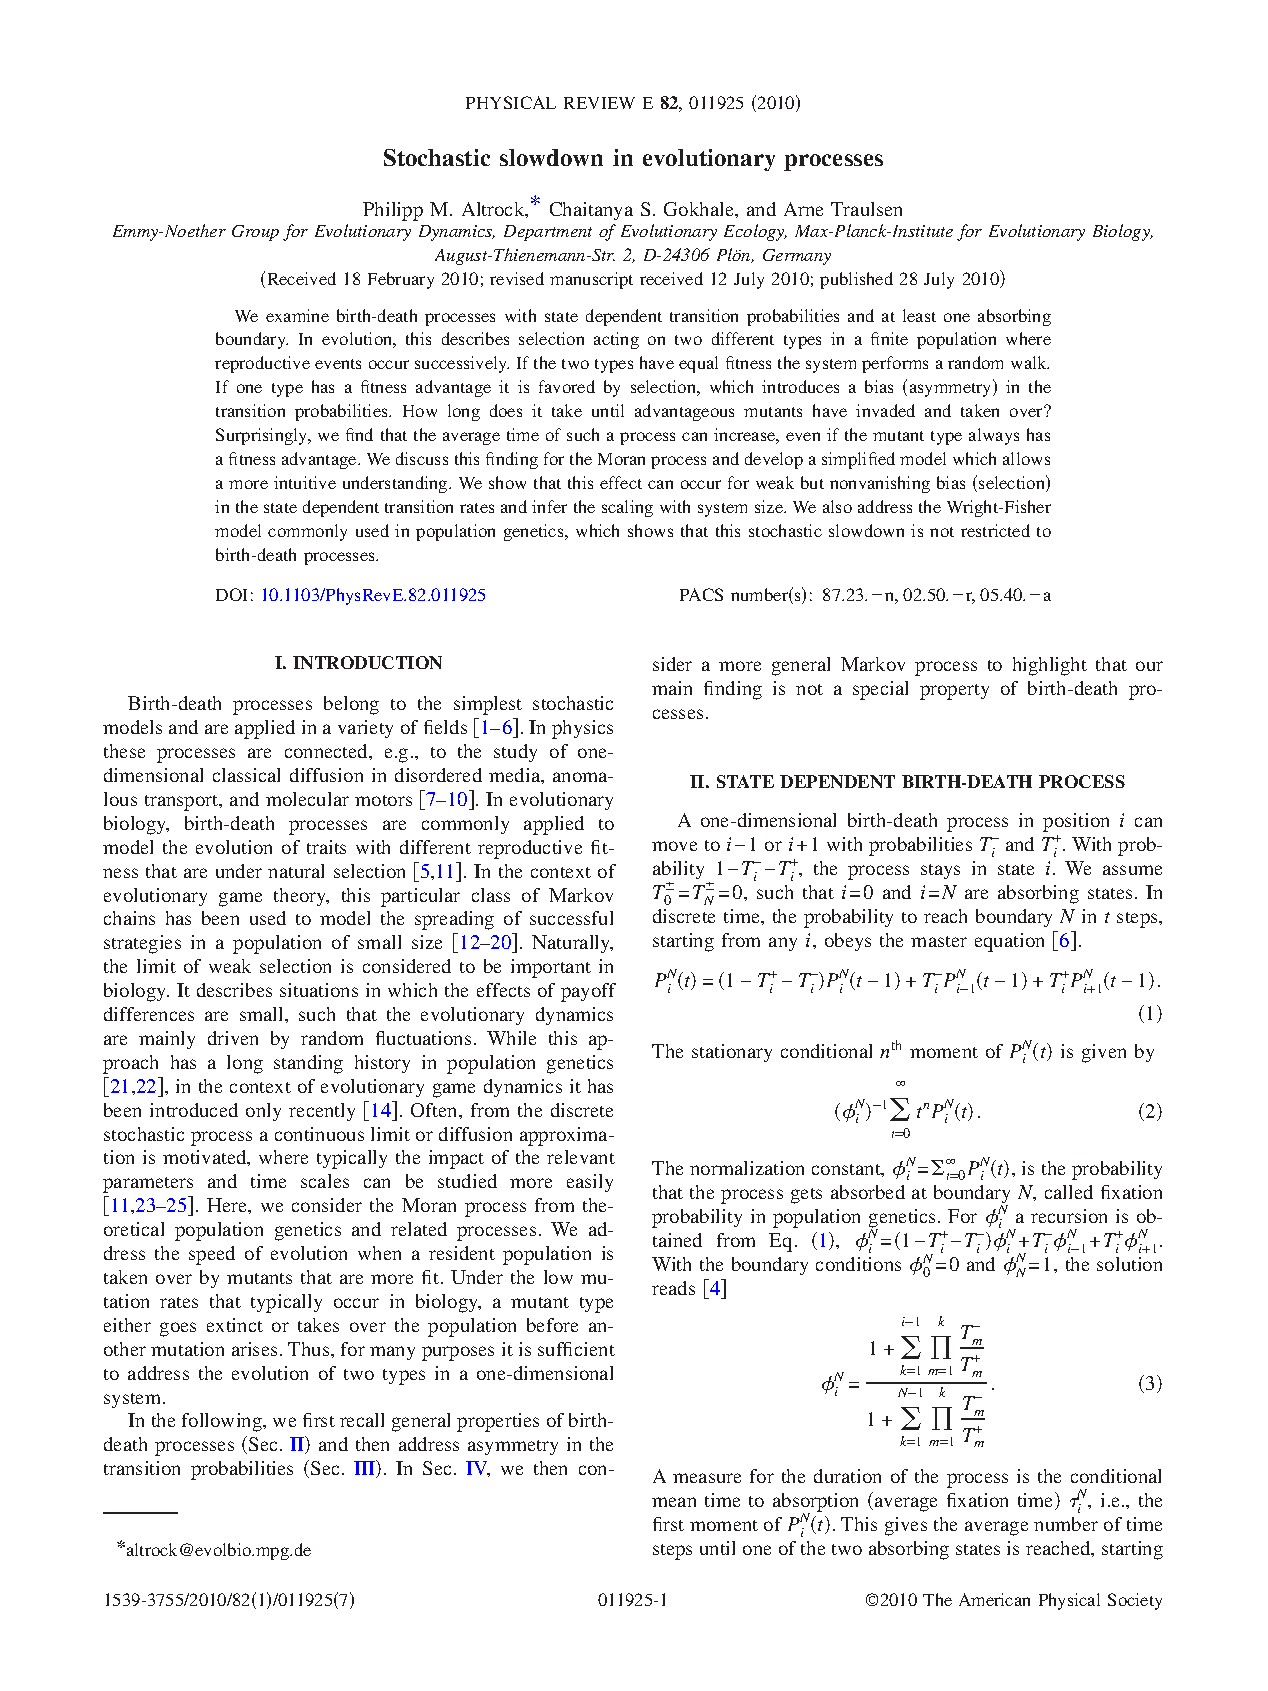
\includepdf[pages=-,scale=0.8]{Papers/Altrock_PRE_2010.pdf}


\begin{savequote}[14pc]
\sffamily
``Any fool can make things bigger, more complex and more violent.
 It takes a touch of genius and a lot of courage to move in the opposite direction"
\qauthor{Albert Einstein (1879-1955)}
\end{savequote}

\chapter{Evolutionary Game Theory}
\label{chap:egttheory}

\graphicspath{{EGTfigs/}{EGTfigs/}{EGTfigs/}}

\section{Introduction}

Frequency dependent fitness introduces a strategic aspect to evolution.
Evolutionary game theory is the study of biological systems with frequency dependent fitness.
Consider the following example.

When introduced, evolutionary game theory was used to model animal conflict situations.
We use a classical example of hawks and doves used by \citet{maynard-smith:1973to}.
When fighting over resources say hawks are the ones who escalate the fight.
Doves do not fight, instead they share the resource equally.
Let the benefit of securing the complete resource be $b$ and the cost for fighting over it be $c$ with the relation $c>b$.
This problem can be represented as,
%
\begin{eqnarray}
\bordermatrix{
&\text{Hawk}&\text{Dove}\cr
\text{Hawk}&\frac{b-c}{2} & b\cr
\text{Dove}& 0 & \frac{b}{2}
}.
\end{eqnarray}
%
The above way of representing the problem is known as the \textbf{payoff matrix}.\index{payoff!payoff matrix}
This particular payoff matrix denotes the payoff for the row player and it reads as follows:
\begin{enumerate}[(1)]
\item \textbf{I (row player hawk) meet another hawk.}
I will keep on fighting until one of us relents.
On winning I will get $b-c$ but as each of us has an equal chance of winning the expected payoff is $(b-c)/2$.
\item \textbf{I (row player hawk) meet a dove.} The opponent being a dove gives in without effort and I get the full benefit $b$ without paying any cost.
\item \textbf{I (row player dove) meet a hawk.} This is the mirror image of $(2)$.
Seeing the Hawk I give in and gain nothing, $0$.
\item \textbf{I (row player dove) meet another dove.} We both do not want to fight and just split the benefit equally between the two of us, each getting, $b/2$.
\end{enumerate}

As $c>b$, that is the benefit from winning does not cover the cost hence a dove does better in a population dominated by hawks.
While the hawks fight each other and get negative payoffs, a dove is better off getting $0$.
Similarly, if all are doves then it pays to be a hawk and get $b$ instead of $b/2$.
Hence there will be a stable co-existence of hawks and doves.
The hawk-dove game is a bit misleading because the interactions are described as between species.
We can consider the types to be behavioural strategies as being aggressive or docile.
Overall this example clarifies the most basic point of evolutionary game theory, frequency dependence.\index{frequency dependence}
This is the essence of evolutionary game theory (see Fig.\ \ref{fig:seesaw}).
%
\begin{figure}[!h]
  \begin{center}
\boxed{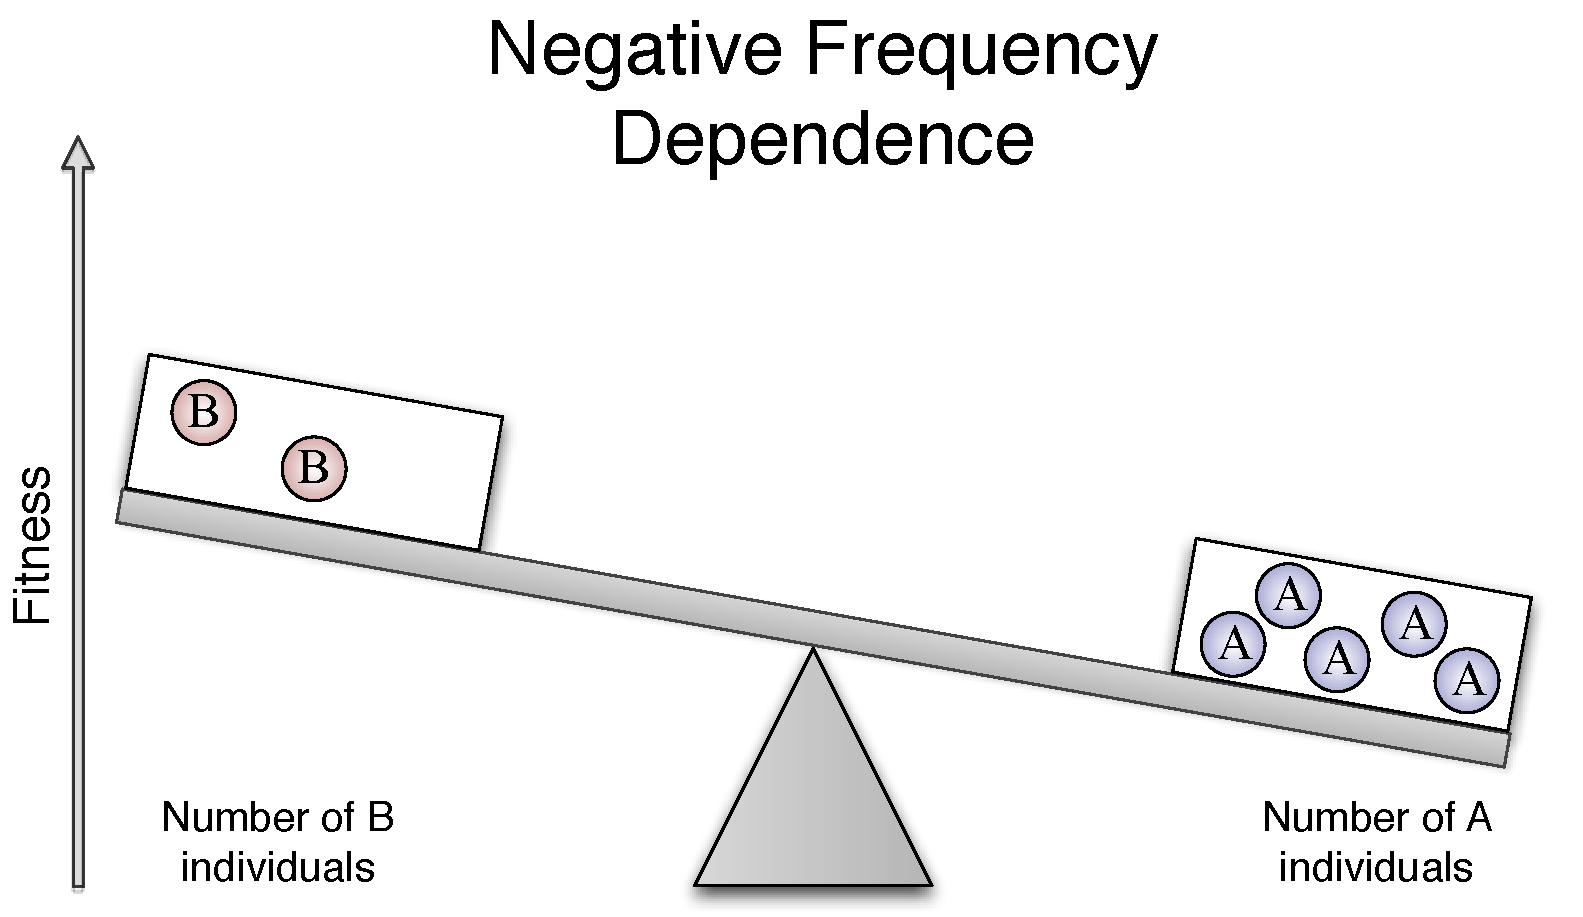
\includegraphics[width=0.9\columnwidth]{seesaw}}
    \caption{\textbf{A seesaw model of negative frequency dependence.}
    \small{If the number of $A$ individuals increases further then the fitness of type $A$ will reduce even more.
    But having a greater fitness in effect means that the number will increase.
    Hence now when the number of $B$ players increases the $B$ side will go down i.e. the fitness of $B$ will go down.
    If we maintain a fixed population size then the increase in $B$ is compensated by a reduction in $A$.
    Thus for a small number of $A$ individuals the fitness of $A$ will be greater than that of $B$.
    This in particular is an example of what is known as negative frequency dependence, where the lower the frequency, the higher the fitness.
    Positive frequency dependence means that as the number increases, fitness increases.
    In general, the position of the pivot is not exactly in the centre.\index{frequency dependence!negative}\index{frequency dependence!positive}}
    }
    \label{fig:seesaw}
  \end{center}
\end{figure}
%
Frequency independence can be a subset of frequency dependence and hence studying frequency independent selection is a simple special case in evolutionary game theory.
But this is an anecdotal explanation and where can it be actually used?

In a recent, resource utilisation experiment with the yeast \textit{Saccharomyces cerevisiae}, conflict between genes SUC2 and suc2 was analyzed
\citep{maclean:2010ye}.\index{\textit{Saccharomyces cerevisiae}}
Two strains of yeast were used.
One with the gene SUC2 secretes an extra-cellular enzyme called invertase which catalyses the hydrolysis of sucrose into glucose and fructose, which can then can be taken up by the cell \citep{greig:2004aa,doebeli:2005aa,gore:2009na}.
The strain with gene suc2 does not secrete invertase.
Thus, suc2 bearers are free from the manufacturing costs but they can utilise the glucose and fructose made by the SUC2 bearing strain
The secretors are termed as ``co-operators", while
non-secretors as ``defectors". 
In \citet{maclean:2010ye} the highest average fitness is obtained in a stable coexistence of the two strains.
Using the published data we can write a payoff matrix for the interactions \citep{wu:2011pr},
%
\begin{eqnarray}
\bordermatrix{
 & \text{SUC2} & \text{suc2} \cr
\text{SUC2} & 0.9475 & 1.03913 \cr
\text{suc2} & 1.03912 & 0.9495 \cr}.
\label{duncan:FitnessMatrix}
\end{eqnarray}
%
We see that it is better to do the opposite of what the other player is doing.
Thus this interaction can be studied as the ``Hawk-Doves problem" encountered earlier.


The first use of indirect game theoretical arguments in biology is attributed to \citet{fisher:1930fi}.\index{Fisher, Ronald}\index{sex ratio}
He was intrigued by the question, why the sex ratio in mammals is usually $1:1$?
He noticed that the fitness of a male is greater in a population consisting of more females than males and vice versa.
The relative frequencies of both the sexes will thus tend to balance each other (the seesaw in Fig.\ \ref{fig:seesaw} would be balanced).
The fitness of a sex depends on its relative frequency in the population.
The use of formal game theoretic arguments in biology was pioneered by R. C. \citet{lewontin:1961to}.
John Maynard Smith championed game theory in biology and described how it can be used to aptly describe animal conflict and other biologically strategic scenarios \citep{maynard-smith:1973to,maynard-smith:1982to}.\index{Maynard Smith, John}
From the interactions between genes or cells \citep{axelrod:2006pn,basanta:2008cp}, between individuals (microbes to humans) or communities \citep{axelrod:1984yo,turner:1999hp,archetti:2000aa,turner:2005aa,frey:2010aa} and even across species like host-parasite interactions \citep{vickery:2010aa}, all can be captured by evolutionary games.

The word `evolutionary' in this sense is not limited to biological evolution but can also describe cultural evolution, dealing with the evolution of behaviours and ideas \citep{hofbauer:1998mm,vincent:2003bo,kandori:1993aa}.
One of the most important applications of evolutionary game theory has been in the research of evolution and maintenance of co-operation and eusociality.
The problem of co-operation is typically represented by a payoff matrix with the following structure,
%
\begin{eqnarray}
\bordermatrix{
 & \text{C} & \text{D} \cr
\text{C} & b-c & -c \cr
\text{D} & b & 0 \cr},
\label{coop:FitnessMatrix}
\end{eqnarray}
%
where $C$ and $D$ stand for the strategies, co-operate and defect.
As earlier the matrix gives the payoffs for the row player.
If the row player is a co-operator then he/she has to pay the cost for co-operation $-c$.
The benefit of co-operation $b$ is obtained only if the other player co-operates.
Since the lower row of the payoffs is consistently higher than the upper row of payoffs, it makes sense for the row player to play the strategy $D$ instead of $C$.
Assuming that the column player is at least as smart as the row player, both of them will choose to play $D$.
The social optimum, where both of them would have co-operated would have resulted in a payoff of $b-c$ to each.
Instead the search for an individual optimum led the players to obtain $0$.

An economic analysis of the scenario clearly reveals that co-operation will be eliminated from the population.
How could then a behaviour which costs the acting individual and benefits another have evolved by natural selection?
In the seminal paper by \citet{axelrod:1981yo} the problem of co-operation was analysed based on artificial players.\index{co-operation!evolution of}\index{co-operation!maintenance of}
\index{co-operation!examples of}
There are numerous examples of co-operation in a natural setting:
\begin{itemize}
\item When viruses infect the same cell they compete for the available resources \citep{turner:1999hp,turner:2005aa}.
``Cheater" viruses get rid of the genes for utilising resources which are available from other viruses and thus prey on the common good.
\item Evolution and maintenance of multi-cellular life forms requires the co-operation of the composing cells \citep{nowak:2006bo}.
Evolution of cancer is about the breakdown of co-operation amongst the cells \citep{dingli:2006cc}.
\item Minnows demonstrate predator inspection behaviour \citep{george:1961aa}.
An ingenious experiment in which sticklebacks inspect a cichlid model was done by \citet{milinski:1987ju,milinski:1988aa,milinski:1990aa} where a pair of fish are locked in a dilemma.
Who will take the greater risk while inspecting the fish?
A similar experiment was carried out in guppies \citep{dugatkin:1988aa,dugatkin:1990aa,dugatkin:1997aa}.
\item Males of the Lance-tailed manakins participate in complex group courtship displays which benefit only the alpha male \citep{duval:2007aa}.
This raises the question of why do the subordinate males take part in the ritual.
\item Blood meal sharing in vampire bats is a classic example where vampire bats can regurgitate blood meal for others who did not get enough \citep{wilkinson:1984sg}.
\item Humans and other social organisms seem to be at the pinnacle of co-operation.
Just as there is rampant incidents of cheating and selfish behaviour, there are also occurrences of long sustained co-operation amongst humans \citep{smith:1776le,wedekind:1996zx,milinski:1998zp,milinski:2001og,fehr:2002bv,fehr:2004pi,sommerfeld:2007fk,henrich:2006lr,sigmund:2007oz,kummerli:2007vl,fehr:2008oz,gachter:2009la,traulsen:2010pn}.
\end{itemize}
%
Using games such as the Prisoners Dilemma, Snowdrift game etc. this problem has been analysed in great depth.
An in-depth discussion on this problem is beyond the scope of this thesis and hence we just briefly refer to this application of evolutionary game theory.
For these and other interesting types of games, see \citet{gintis:2000bo} or \citet{sigmund:2010bo}.

The names of these games come from short anecdotes like the ``Hawk-Dove".
They represent human economic conflict situations as was useful in classical game theory.
Maynard Smith took the notations from classical game theory \citep{neumann:1944ef} like the payoff matrix but developed a new logic for the analysis of games in a biological context.
The games could be thus used as a proxy for animal conflict situations \citep{maynard-smith:1973to}.
The development of evolutionary game theory is split into two parts, the static analysis initialised by Maynard Smith and the dynamical analysis  developed by \citet{taylor:1978wv}, \citet{zeeman:1980ze}, \citet{schuster:1983le}, \citet{hofbauer:1985jm} and \citet{hofbauer:1988mm}, as well as many others.

\section{Evolutionarily Stable Strategies}
\label{sec:ess}
\index{evolutionarily stable strategies}
In ``The Logic of Animal Conflict" published by John Maynard Smith and George Price in Nature in 1973, they introduce a condition for a strategy to be evolutionarily stable.
But what does it mean to be evolutionarily stable?
To get to the heart of the question we do away with particular examples.
In an abstract way consider just two strategies $A$ and $B$.
In an infinite population of $A$ players imagine that a very small fraction of them start playing strategy $B$.
What is the condition for $A$ to oppose this invasion of $B$?
If we find a certain condition and $A$ satisfies that condition then we say that strategy $A$ is an \textit{evolutionarily stable strategy} (ESS).

Let us find this condition.
As before we write down a payoff matrix for the game\index{payoff!payoff matrix},
%
\begin{eqnarray}
\label{eq:paymat}
\bordermatrix{
&A&B\cr
A&a_1 & a_0\cr
B& b_1 & b_0
}.
\end{eqnarray}
%
The matrix denotes the payoffs for the row player.
The payoff entries are written so that we immediately know where they belong in the matrix.
The small $a$ is a payoff entry for strategy $A$ and the subscript denotes if the other player is $A$, given by $1$, or not, given by $0$.
Now from this infinitely large population let the frequency of the players playing strategy $A$ be $x$.
Hence the frequency of players playing strategy $B$ is given by $1-x$.
The game matrix denotes the interaction of two players.
Hence an $A$ player can meet another $A$ player or a $B$ player.
The probability of meeting a player of a certain strategy is the frequency of that strategy.
This is because we have assumed a well mixed population \citep{maynard-smith:1973to}.
In genetical terms this would mean random mating.
For example when an $A$ player meets another $A$ player (this will be with probability $x$) then the focal $A$ player gets $a_1$ according to the payoff matrix.
From this we can calculate the average payoffs to both the strategies, namely $\pi_A$ and $\pi_B$ as,\index{payoff!average payoff}
%
\begin{eqnarray}
\label{infinitepayoffs}
\pi_A &=& a_1 x + a_0 (1-x) \\
\pi_B &=& b_1 x + b_0 (1-x) .
\end{eqnarray}
%
If the average payoff of strategy $A$ is always larger than that of strategy $B$ then $B$ will not be able to invade $A$,
%
\begin{eqnarray}
\pi_A &>& \pi_B \nonumber \\
a_1 x + a_0 (1-x) &>& b_1 x + b_0 (1-x).
\label{ineq1}
\end{eqnarray}
%
Since we have assumed that the frequency of the invading $B$ players is very small, we can cancel the terms with $1-x$ as $x \approx 1$.
Thus we arrive at the condition,
%
\begin{equation}
a_1 > b_1
\end{equation}
%
If we are dealing with a quirky situation where $a_1 = b_1$, then we need to restart our analysis at the earlier inequality \eqref{ineq1}.
In this case we cancel $a_1$ terms with $b_1$ terms and are left with the condition,
%
\begin{equation}
a_0 > b_0 \ \ \ \ (\text{given that } a_1 = b_1)
\end{equation}
%
Thus for strategy $A$ to be an \textbf{ESS} either of the following conditions must be met,
%
\begin{itemize}
\item $a_1 > b_1$ or $a_1 = b_1$ and $a_0 > b_0$.
\item $a_1 > b_1$ or $a_1 = b_1$ and $a_0 \geq b_0$ also termed as \textbf{``weak ESS"} \citep{thomas:1984aa,thomas:1985aa}.
\end{itemize}
%
An intuitive understanding of an ESS is that a focal strategy ($A$) has to do better when playing against itself ($A$) than when compared to another strategy ($B$) playing against the focal strategy ($A$).
If somehow this barrier is broken and the invading strategy ($B$) pushes through, then the focal strategy ($A$) should do better when playing against the invading strategy ($B$) as compared to the invading strategy ($B$) against itself ($B$).
%
\begin{figure}[h]
  \begin{center}
      \boxed{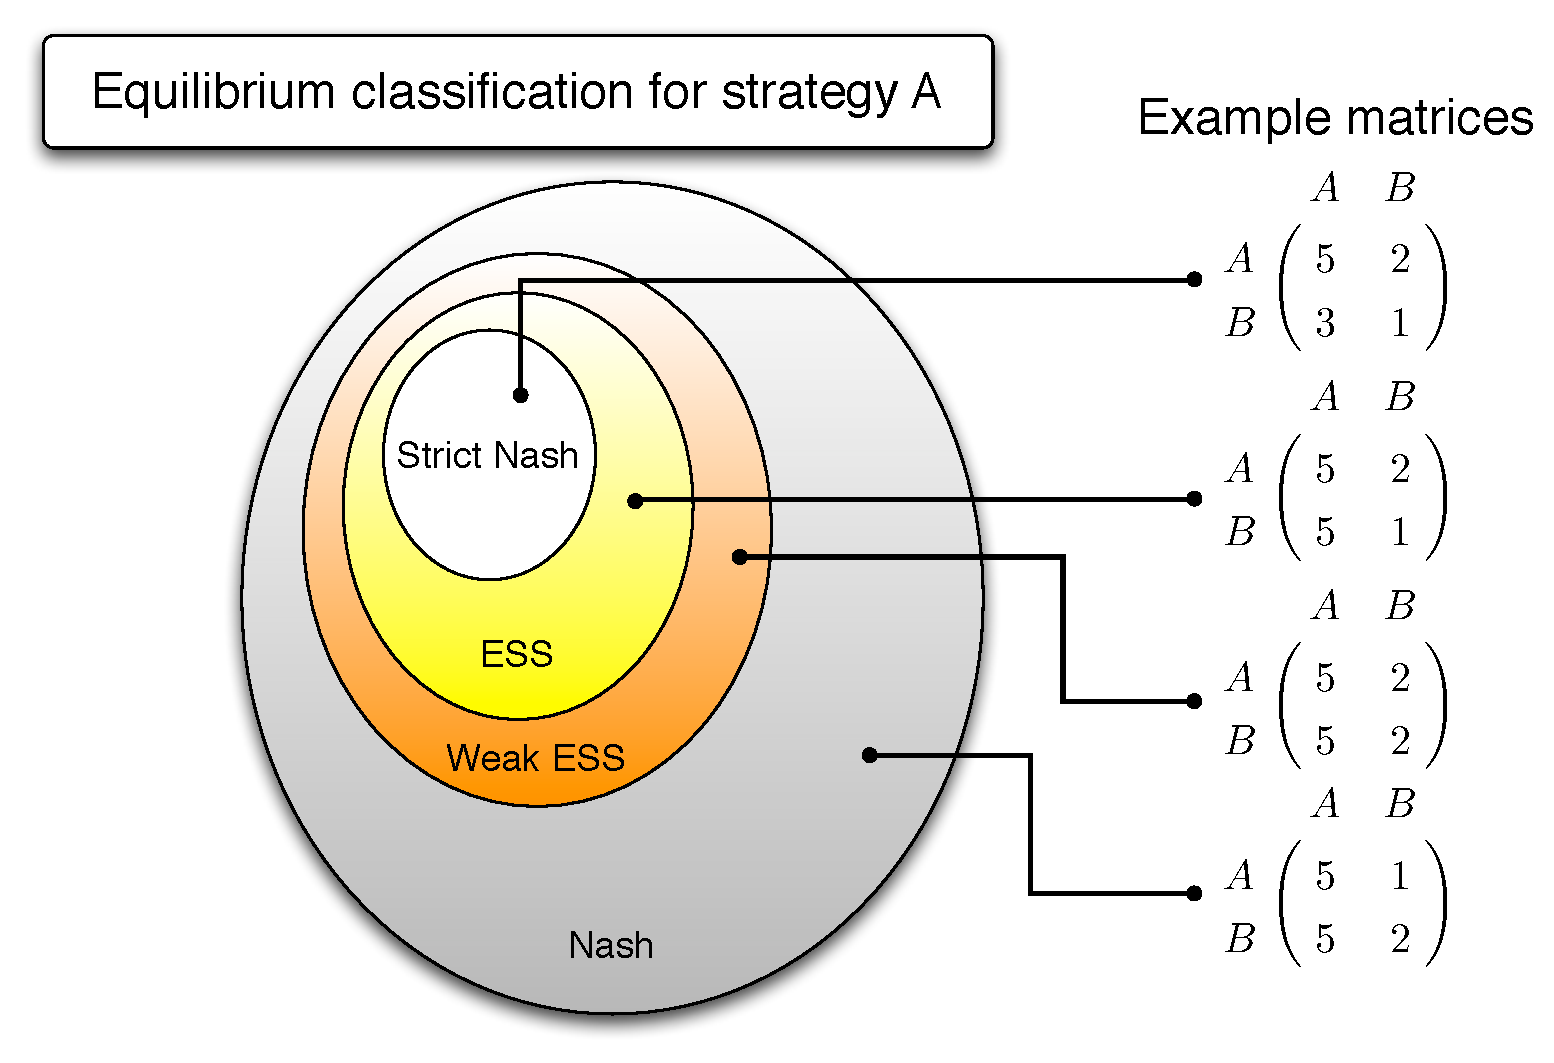
\includegraphics[scale=0.5]{ESSNE}}
    \caption{\textbf{Equilibrium classification for strategy $\mathbf{A}$.}
    \small{Denoting the logical relationships between ESS and Nash equilibria.
    All strict Nash equilibria are ESS which are all weak ESS which are all Nash but the reverse is not always true.}
    }
    \label{fig:essnash}
  \end{center}
\end{figure}
%
\index{evolutionarily stable strategies}
\index{Nash, John!Nash equilibrium}

There is a deeper relationship between ESS and the traditional concept of Nash equilibrium \citep{nash:1950ef} (see Fig.\ \ref{fig:essnash}).\index{Nash, John!Nash equilibrium}
In classical game theory strategy $A$ would be a \textbf{strict Nash} equilibrium when an $A$ playing against itself is better than $B$ playing against $A$ i.e. $a_1 > b_1$.
Strategy $A$ is a \textbf{Nash} equilibrium if it performs against itself at least as well as $B$ performs against it, i.e. $a_1 \geq b_1$.
A Nash equilibrium in short is the equilibrium from where no player can improve his or her payoff by switching strategies unilaterally \citep{nash:1950ef}.\index{Nash, John!Nash equilibrium}

The ESS analysis tell us whether a particular configuration of the population is resistant to invasion by a small number of mutants.
But how do we know if the population can even reach that configuration in the first place?
For this we look at the dynamics of the system.

\newpage
\section{Evolutionary Game Dynamics}
\label{sec:EGD}
Traditionally evolutionary game theory deals with phenotypic traits.
\textit{``Evolutionary game theory, [$\ldots$], describes evolution in phenotype space"} \citep{nowak:2004aa}.
The different phenotypic traits are termed as strategies (like the earlier secretors and non-secretors).
In this section we describe the dynamics of such strategies.
Although evolutionary game theory is developed from the theory of games in economics \citep{neumann:1944ef}, it forgoes an important assumption of game theory: rationality.
In evolutionary game theory natural selection is the dominant force.
Individuals are born with fixed strategies.
They interact with each other and receive payoffs according to a payoff matrix based on their strategies.
Strategies which get the higher payoff are said to be more successful than those which do not.
These successful strategies spread in the population at the cost of other weaker strategies.
Understanding this process is the mainstay of evolutionary game dynamics \citep{sandholm:2010bo}.
\\

\fcolorbox{red}{Light}{\parbox{0.9\textwidth}{
\textbf{Difference and Differential equations (Box \ref{diffeqbox})}\\
\label{diffeqbox}
\ \ \ \ Before delving into game dynamics let us turn back to Malthus for a moment.
Malthus proposed one of the earliest models of population growth now known as the Malthusian growth model or often the simple exponential growth model.
\index{Malthus Thomas}
\index{dynamical system!difference equation}
\index{dynamical system!differential equation}

\ \ \ \ Consider an organism which increases in number exponentially ($e$-fold) at every time step.
If the number of organisms at time $t$ is $p_t$ then the number at the next time step $t+1$ is given by,
%
\begin{equation}
p_{t+1} = e p_t
\end{equation}
%
If we know the initial condition, i.e. the number at $t=0$ then we can calculate the number of organisms at any time $t$ exactly as,
%
\begin{equation}
p_{t} = e^t p_0
\end{equation}
%
This type of equation is known as a difference equation as it uses the information from discrete time-points and calculates the differences to arrive at the final position specified in this example by $t$.

\ \ \ \ If time is measured continuously rather than in discrete time steps then we use a differential equation instead of a difference equation.
For the above type of system we can write a differential equation as,
%
\begin{equation}
\frac{dp} {dt} = r p 
\end{equation}
%
For the sake of concise notation we use $\dot{p} = \frac{dp} {dt}$, where the dot denotes the derivative taken with respect to time.
The solution of this differential equation is obtained by integrating it, which leads to,
%
\begin{equation}
p(t) = e^{r t} p(0),
\end{equation}
%
where $p(t)$ and $p(0)$ are the frequencies at the respective time points.
}
}
\\

\citet{taylor:1978wv} and \citet{zeeman:1980ze} extended the realm of evolutionary game theory to include dynamics.
This was a major leap forward in the field of evolutionary game theory.
They introduced a differential equation (see Box \ref{diffeqbox}) based on the quasi-species equation \index{quasi-species!quasi-species equation}initially developed by \citet{eigen:1977aa} \citep{eigen:1989aa}.\index{Eigen, Manfred}\index{Schuster, Peter}\index{quasi-species!quasi-species equation}
The quasi-species equation\index{quasi-species!quasi-species equation} does not include frequency dependent fitness but mutations.
Excluding mutations but including frequency dependent fitness we arrive at the replicator equation (see Fig.\ \ref{fig:equations}).\index{replicator!replicator equation}
A simultaneous generalisation of these two equations leads to the replicator-mutator equation \index{replicator!replicator-mutator equation} which includes frequency dependent fitness as well as mutations \citep{stadler:1992wv,bomze:1995rm,nowak:2001ln,page:2002an} (see Fig.\ \ref{fig:equations}).
All these equations tell us how the strategies replicate and how their frequencies change over time.
%
\begin{figure}[h]
  \begin{center}
    \boxed{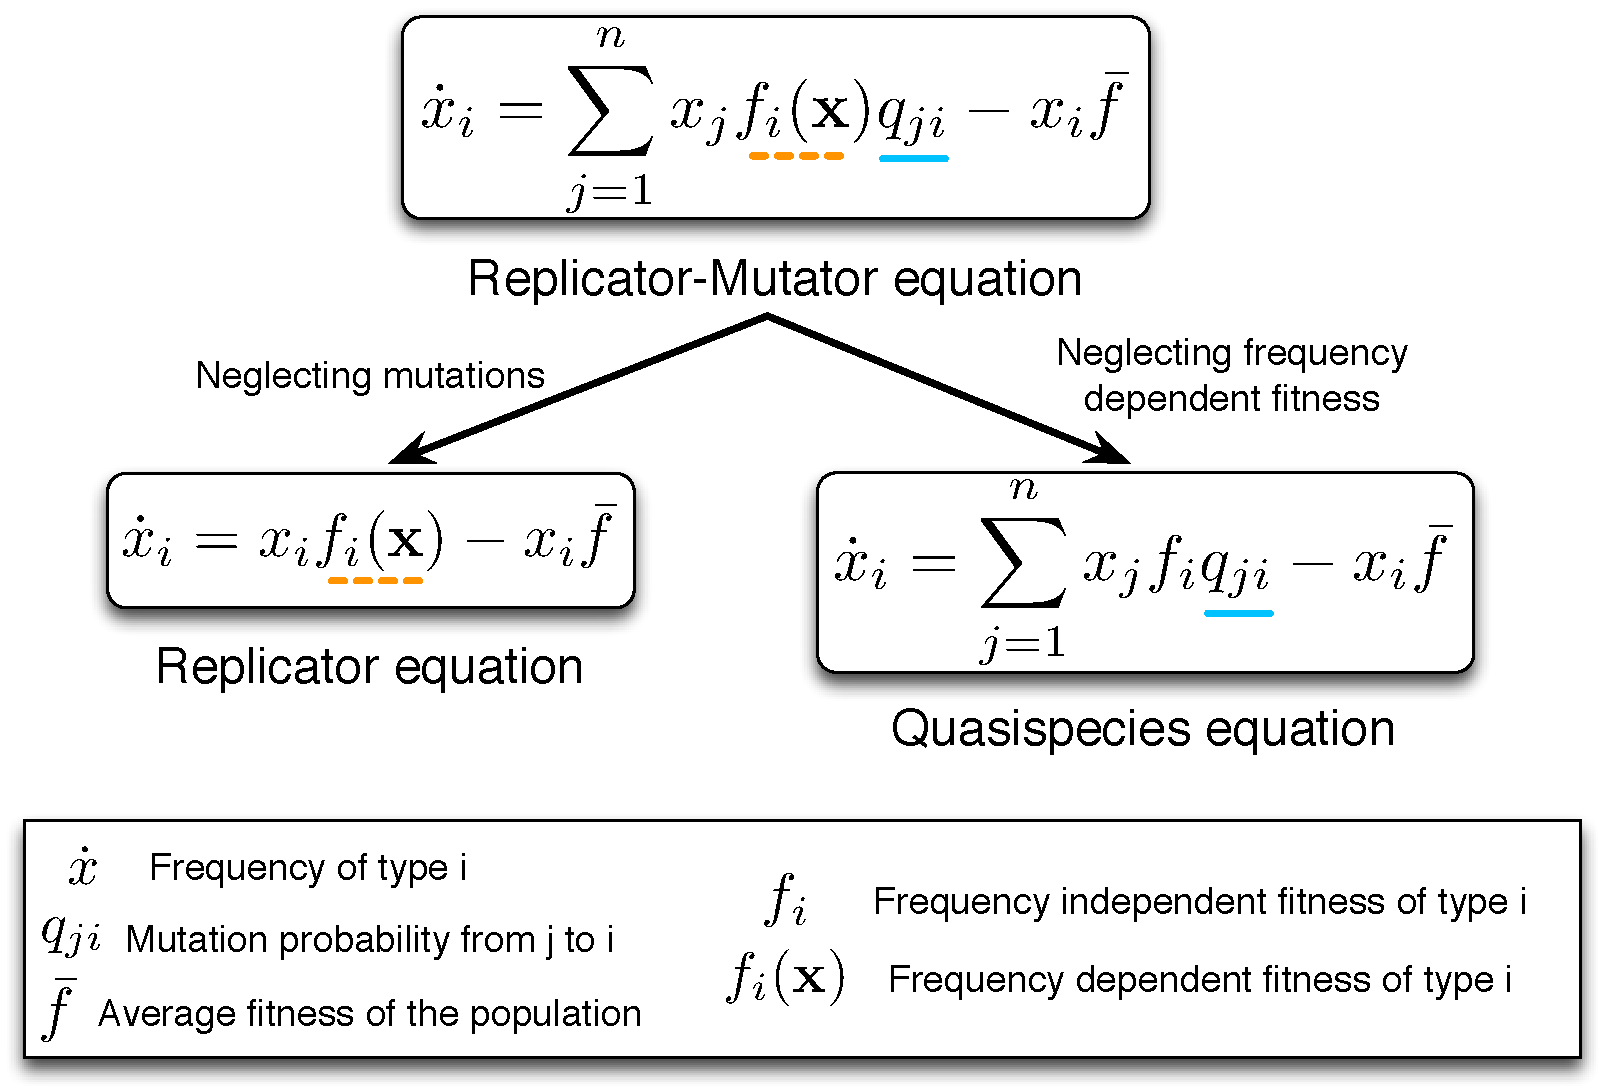
\includegraphics[width=0.8\columnwidth]{equations}}
  \end{center}
  \caption{
  \label{fig:equations}
  \textbf{Replicator and quasi-species equations\index{quasi-species!quasi-species equation} as special cases of the Replicator-Mutator equation\index{replicator!replicator-mutator equation}.}
  \small{The quasi-species equation\index{quasi-species!quasi-species equation} includes mutations between types but the fitness of the types are frequency independent.
  In the replicator equation the fitnesses  of types is frequency dependent but there is no chance for mutations.
  Hence while a certain type can go extinct in replicator dynamics it may not in quasi-species\index{quasi-species!quasi-species dynamics} dynamics if it is fuelled by mutations from some other type.
  Including both frequency dependent and mutations leads to the replicator-mutator equation.}
  }
\end{figure}
%
\newpage

\subsection{Replicator Dynamics}

At the core of evolutionary game theory lies the replicator equation. \index{replicator!replicator equation}
The replicator equation allows the frequencies of the different types in the population to determine the fitness landscape rather than setting the fitness of each type to be constant (Constant fitness is a special case of the replicator dynamics).

Let us take a bottom-up approach to the replicator equation.
As before, consider two types in an infinitely large population, $A$ and $B$.
The frequency of type $A$ is given by $x_A$ and that of type $B$ by $x_B$.
Since these are the only two types in the population, the frequencies sum up to one, i.e. $x_A + x_B = 1$.
Each type has an average fitness denoted by $f_A$ and $f_B$.
How this fitness is actually derived is a question pertaining to the particular context of the model we are studying.
For our purpose we just consider fitness in its meaning, a quantitative measure of the ability of that type to pass on to the next generation.
We consider the case of frequency dependent fitness.
Hence we have $f_A (\mathbf{x})$ and $f_B (\mathbf{x})$ as the fitnesses.
The bold $\mathbf{x}$ denotes that it is a vector, a set of frequencies of both the types ($\mathbf{x} = \{x_A,x_B\}$), as the fitness can depend on the frequencies of both the types.
Considering the classical selection ideas we know that if this fitness is greater than the average fitness of the population then the frequency of that type increases over time and vice versa.
Using this information we write down a set of two differential equations for the two types as follows,
%
\begin{eqnarray}
\label{eq:rep1}
\dot{x}_A &=& x \left(f_A (\mathbf{x}) -\bar{f} \right) \\
\dot{x}_B &=& y \left(f_B (\mathbf{x}) - \bar{f} \right).
\end{eqnarray}
%
We keep the population size constant by defining $\bar{f} = x_A f_A + x_B f_B$.
This is just the average fitness of the population.
Since we know that there are only two types in the population, we have $x_B=1-x_A$.
Substituting these values of $\bar{f}$ and $x_B$ in Eq.\ \eqref{eq:rep1} we can use only one equation instead of the two to describe the dynamics of the whole system,
%
\begin{eqnarray}
\dot{x}_A &=& x_A (1-x_A) \left[f_A (\mathbf{x}) - f_B (\mathbf{x}) \right].
\end{eqnarray}
%
For the sake of simplicity we consider $x = x_A$ and thus $x_B=1-x$.
Also remembering that the fitnesses are frequency dependent, we drop the functional notation of the fitnesses and write a cleaner equation as,
%
\begin{eqnarray}
\label{eq:simplerep}
\dot{x} &=& x (1-x) \left(f_A - f_B \right).
\end{eqnarray}
%
Here, one differential equation suffices.
In general, if we have $n$ different types in the population then we need a system of $n-1$ differential equations,
%
\begin{eqnarray}
\label{eq:repeq}
\boxed{ 
\dot{x}_i = x_i \left[f_i (\mathbf{x}) - \bar{f} \right]
}
\end{eqnarray}
%
where $i = 1,2,\ldots n-1$ and the average population fitness is now $\bar{f} = x_1 f_1(\mathbf{x}) + x_2 f_2(\mathbf{x}) \ldots + x_n f_n(\mathbf{x}) = \sum_{i=1}^{n} x_i f_i (\mathbf{x})$ where $x_i$ and $f_i$ is the frequency and fitness of type $i$ respectively.
This is the replicator equation\index{replicator!replicator equation}.

The solution of the replicator equation can be viewed in a $n-1$ dimensional space.
For example, the solution for a two type case can be plotted on a single line, for three types we would need a two dimensional space and so forth.
This way of representing the solution space is known as a simplex (see Box \ref{simplexbox}).\index{dynamical system!simplex}
\\

%
\fcolorbox{red}{Light}{
\parbox{0.9\textwidth}{
\textbf{Simplex (Box \ref{simplexbox})}\\
\label{simplexbox}
\index{dynamical system!simplex}
\ \ \ \ In dynamical systems a simplex is a tool for visualizing how the dynamics of a system proceeds.
We saw how the replicator equation can be used to study the dynamics of systems with $n$ different types.
%
\begin{wrapfigure}{l}{0.5\textwidth}
  \begin{center}
    \boxed{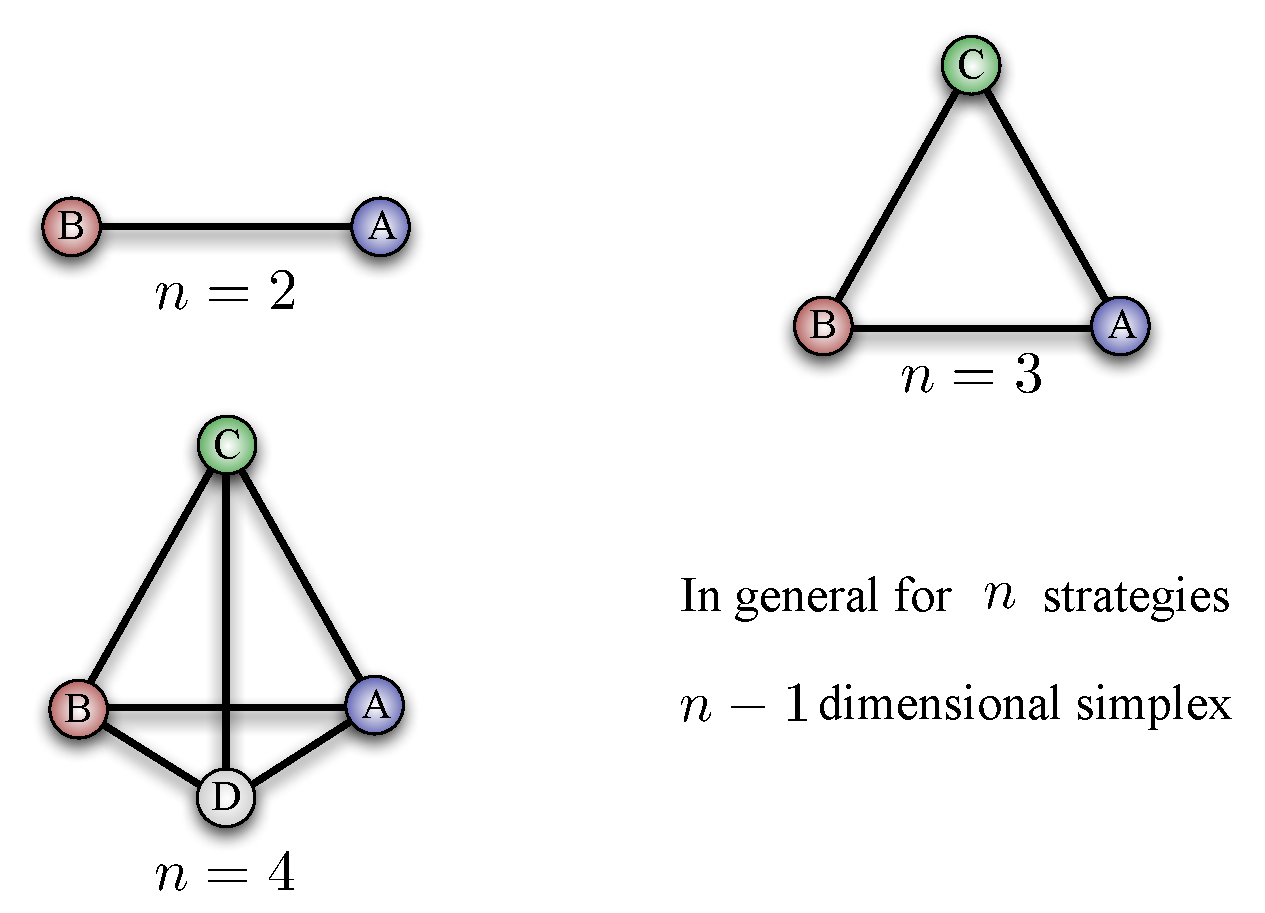
\includegraphics[width=0.48\textwidth]{simplexes}}
  \end{center}
  \caption{
  \label{simplexes}
  \footnotesize{A system with $n$ types can be represented by an $n-1$ dimensional simplex.
  For $n=2$ the simplex is a line.
  For $n=3$ an equilateral triangle and for $n=4$ a tetrahedron.}
  }
\end{wrapfigure}
%
For simplicity consider $n=2$ and let the two types be $A$ and $B$ as considered earlier.
We can represent the state of the population by the frequencies of these two types.
Either the population can be homogeneous for $A$ (i.e. $x_A = 1$ and $x_B = 0$) or for $B$ i.e. $x_A = 0$ and $x_B = 1$.
Consider these two states to be represented by two points.
The line joining them denotes the different possible compositions of the population.
For example at the midpoint of the line, both the types will have the same frequency i.e. $x_A = x_B = 0.5$.

\ \ \ \ Now if we consider $n=3$, with three types $A$, $B$ and $C$ then we represent it by a two dimensional simplex, an equilateral triangle.
Again the midpoint of the simplex is where the frequencies are equal, i.e. $x_A = x_B = x_C = 1/3$.

\ \ \ \ An Italian statistician Bruno de Finetti used the triangular simplex to graph the frequencies of the genotypes for a diploid population with two alleles.
In that sense the vertices correspond to the states where the population is homogeneous for a genotype (say $aa$, $AA$ or $aA$).
This simplex is known in population genetics as the de Finetti diagram.
\index{dynamical system!simplex!de Finetti diagram}
}
}
%
\\

In 1983, Peter Schuster and Karl Sigmund unified fields ranging from ecology to population genetics and prebiotic evolution to sociobiology in their most basic theoretical characteristic \citep{schuster:1983le}.
All these fields are essentially dynamical systems.
Schuster and Sigmund abstracted out the essence of these systems and looked plainly at the dynamics.
They pointed out that all these different models lead to the same class of differential equations and thus a unified equation could be used to describe the essence of these systems.
They named it the replicator equation by taking inspiration from the notion of `replicators' from \citet{dawkins:1982da}.
Further \citet{hofbauer:1998mm} also showed that the set of replicator equations for $n$ strategies are mathematically equivalent to the well known Lotka Volterra equations for $n-1$ species in ecology.
The dynamical equations developed by Lotka and Volterra pre-date the replicator equation by almost half a century \citep{lotka:1920pn,volterra:1928aa}.
In a sense, \textit{``Ecology is the godfather of evolutionary game theory"} \citep{hofbauer:1998mm}.
\index{Lotka, Alfred}
\index{Volterra, Vito}
\index{Lotka-Volterra equations}

Ultimately what the equations tell us is that the change in frequency of a certain type over time depends on its frequency, fitness and the average fitness of the population.
If $f_i (\mathbf{x}) - \bar{f} > 0$ then the frequency will increase over time.
If $f_i (\mathbf{x}) - \bar{f} < 0$ then it will decrease.

Due to this generality of the replicator equations we have not called the different types as ``strategies".
They will be considered as strategies once we connect this dynamical framework to evolutionary game theory.
The evolutionary game is introduced in the dynamics via fitness.
\index{fitness}

\subsubsection{Two strategies}

We have defined fitness to be a function of the frequency of the different types.
In section \ref{sec:ess} we encountered a similar entity, payoffs, denoted by Eqs.\ \eqref{infinitepayoffs}.
For completeness let us repeat the equations,
%
\begin{eqnarray}
\pi_A &=& a_1 x + a_0 (1-x) \nonumber \\ 
\pi_B &=& b_1 x + b_0 (1-x). \nonumber
\end{eqnarray}
%
The coefficients belong to a two player game matrix with two strategies i.e. a $2 \times 2$ game.
In the simplest case we consider the fitness of a strategy to be the payoff (which is already frequency dependent).
Thus,
%
\begin{eqnarray}
f_A &=& \pi_A \\
f_B &=& \pi_B.
\end{eqnarray}
%
The dynamical equation for two strategies is as given earlier by Eq.\ \eqref{eq:simplerep},
%
\begin{eqnarray}
\dot{x} &=& x (1-x) \left(f_A - f_B \right) \nonumber
\end{eqnarray}
%
where $\dot{x}$ describes the change in the frequency of strategy $A$.

Of particular interest are the cases when $\dot{x} = 0$.
This means that the frequency of $A$ does not change.
Hence the system has reached an equilibrium.
Thus we look when $\dot{x} = 0$, which is equivalent to,
%
\begin{eqnarray}
x (1-x) (f_A - f_B) = 0
\end{eqnarray}
%
There are three possible solutions to this equation,
strategy $A$ goes extinct, $x=0$ or the whole population consists of $A$ players, $x=1$ and lastly when the two strategies have equal fitness, $f_A = f_B$ \citep{bishop:1976aa}.
Graphically we can plot the equation and see when it is equal to zero (see Figs.\ \ref{fig:dominance} and \ref{fig:codom}).
As $x$ increases, if the solution of the replicator equation intersects the zero line from above, then the intersection is known as a stable equilibrium (filled circle Figs.\ \ref{fig:dominance} and \ref{fig:codom}).
If instead it intersects from below then it is an unstable equilibrium (open circle Figs.\ \ref{fig:dominance} and \ref{fig:codom}).
In other words, if the derivative of the solution at the intersection is negative then the equilibrium is stable, if it is positive then it is unstable.
For a small perturbation from the stable equilibrium the system returns to the stable equilibrium.
For a small perturbation from an unstable equilibrium the system runs away from the unstable equilibrium in the direction of the perturbation.
\index{dynamical system!stability analysis}


The possible outcomes can thus be represented using the simplices (see Box \ref{simplexbox}) as shown in Figs.\ \ref{fig:dominance} and \ref{fig:codom}.
What do these outcomes mean in terms of the evolutionary game?

\begin{enumerate}[(i)]
\item \textbf{Dominance}
	\begin{enumerate}
	\item Dominance of $A$.
	The population will eventually lead to a state where everyone is playing strategy $A$.
	This is possible if $a_1>b_1$ and $a_0>b_0$.
	This leads to $f_A > f_B$.
	Intuitively it means that it is always better to play strategy $A$ regardless of which strategy the other player is playing (Fig.\ \ref{fig:dominance} (a)).
	\item Dominance of $B$.
	This is a mirror image of the earlier case.
	In this situation it is always better to play strategy $B$ i.e. the fitness of strategy $B$ is always greater than that of $A$, $f_A < f_B$.
	This will be true if $a_1<b_1$ and $a_0<b_0$ (Fig.\ \ref{fig:dominance} (b)).
	\end{enumerate}
	%%
\begin{figure}[!h]
  \begin{center}
    \boxed{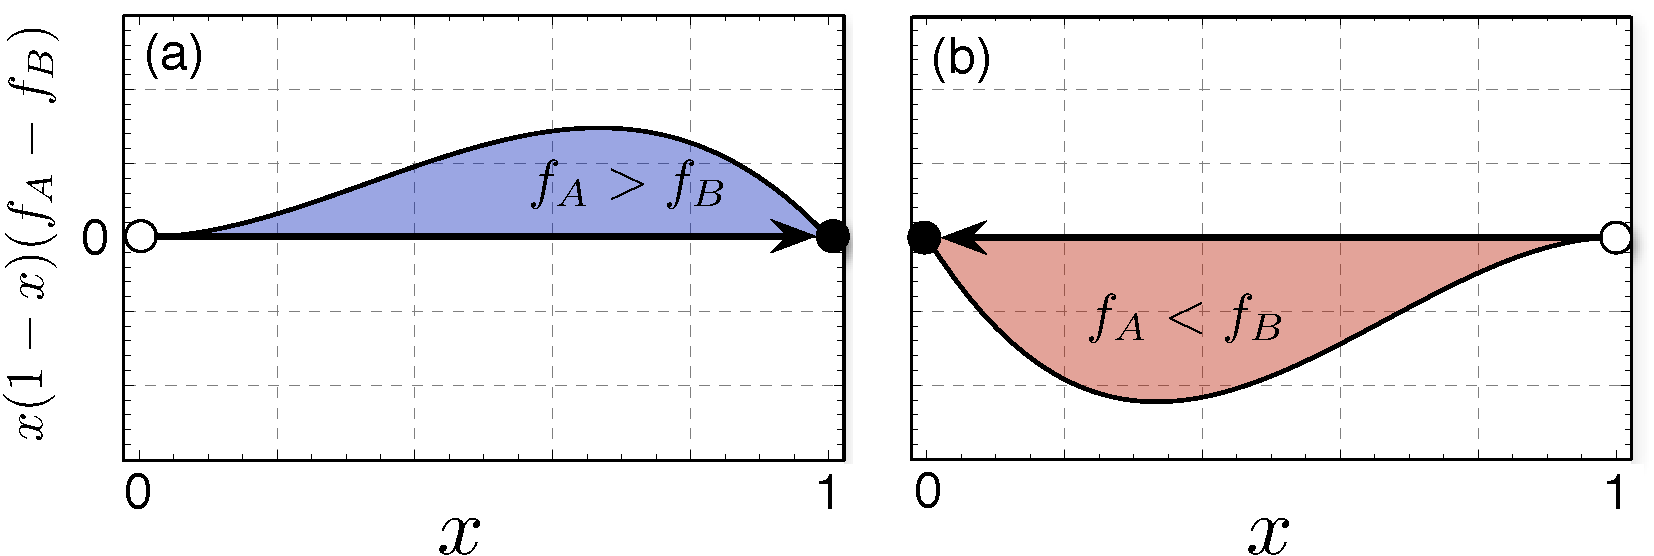
\includegraphics[width=0.9\columnwidth]{dominancerep}}
  \end{center}
  \caption{
  \label{fig:dominance}
  \textbf{Examples of dominance in a two player game with two strategies.}
  \small{Let $x$ be the frequency of strategy $A$.
  Scenario (a) is possible when either strategy is always fitter than the other, $A$ fitter than $B$ for (a) and vice versa for (b).
In the simplex notation, the filled dots are the stable equilibria and the unfilled dots are the unstable equilibria.
The arrows shows the direction of selection.}
  }
\end{figure}
%
\item \textbf{Coexistence}. 
	Co-existence of two strategies is possible if each strategy has an advantage when rare.
	When $A$ is rare then we have $f_A > f_B$ but when $A$ becomes abundant then $f_A < f_B$.
	That is when $a_1<b_1$ and $a_0>b_0$.
	It means that it is always best to play the strategy which is not being played by the other player (Fig.\ \ref{fig:codom} (a)).
	%
\begin{figure}[!h]
  \begin{center}
    \boxed{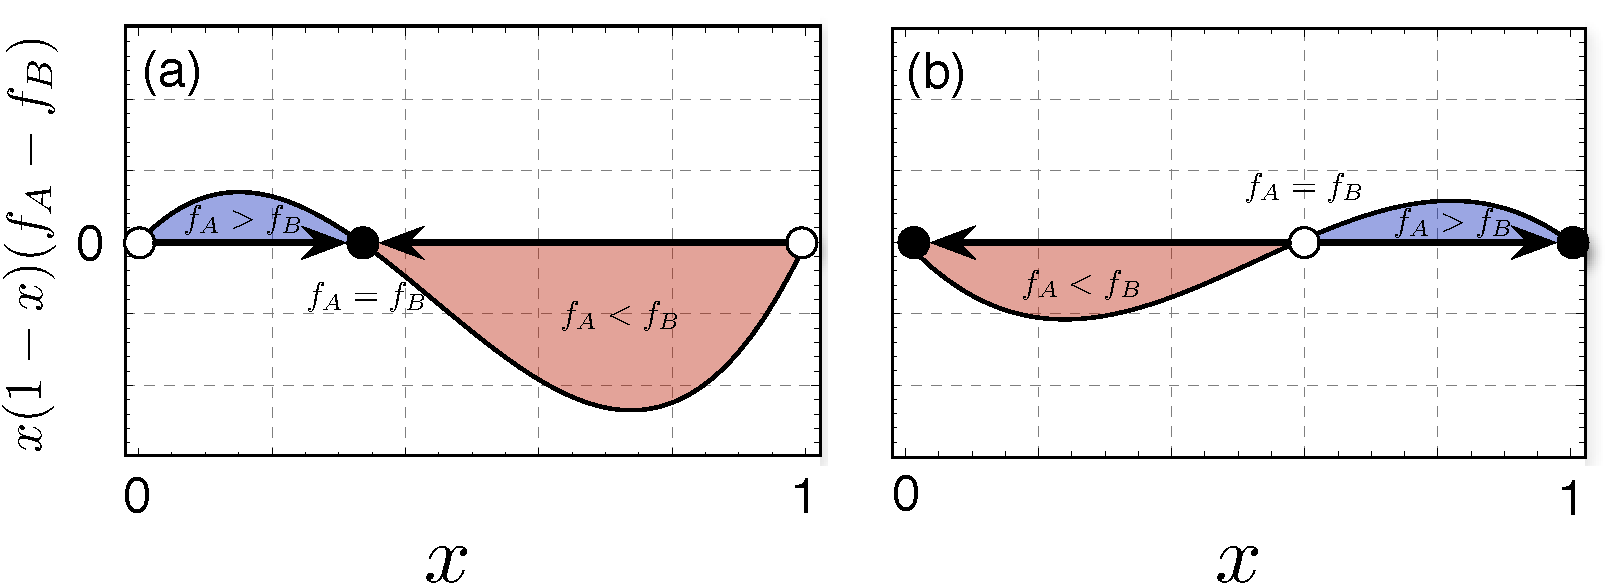
\includegraphics[width=0.9\columnwidth]{codomrep}}
  \end{center}
  \caption{
  \label{fig:codom}
  \textbf{Examples of co-existence and bi-stability in a two player game with two strategies.}
  \small{Let $x$ be the frequency of strategy $A$.
  (a) If each strategy is fitter than the other when it is rare then this leads to the co-existence of the two strategies.
(b) Bi-stability is observed when above a certain frequency of $A$ (open circle), $A$ does better and below it $B$ does better i.e. scenario (b).
As in the earlier figure, the filled dots are the stable equilibrium and the unfilled are the unstable.
The arrows shows the direction of selection.}
  }
\end{figure}
%
\item \textbf{Bi-stability}.
	Bi-stability refers to the condition where the pure states of the system, all $A$ and all $B$, are stable.
	This is possible when a strategy has an advantage when abundant.
	That is $f_A > f_B$ when $A$ is abundant but $f_A < f_B$ when it is rare.
	In this situation it is profitable to play the same strategy as your opponent as $a_1 > b_1$ and $a_0<b_0$ (Fig.\ \ref{fig:codom} (b)).
\item \textbf{Neutrality}.
	Under neutrality both the strategies do equally well and it does not matter which strategy we use.
	The payoffs you get when playing either strategy are equal irrespective of the strategy of your opponent.
	Hence $a_1 = b_1$ and $a_0 = b_0$.
	This leads to $f_A = f_B$.
\end{enumerate}
%
For co-existence and bi-stability we see that the inequality between the fitnesses of the two strategies changes sign.
The exact frequency of strategy $A$ where this switch occurs can be explicitly calculated (the filled circle in Fig.\ \ref{fig:codom} (a) and the open circle in Fig.\ \ref{fig:codom} (b)).
Let us call this frequency $x^*$.
If the system is at that exact point then the fitnesses of both strategies are equal, $f_A = f_B$.
Equating the two fitnesses, $f_A = f_B$, we get,
%
\begin{eqnarray}
x^* = \frac{b_0 - a_0}{a_1 -a_0 -b_1 +b_0} 
\label{inteq}
\end{eqnarray}
%
This frequency of strategy $A$, $x^*$ is the turning point of the dynamics.
For a coexistence game if the frequency of $A$ drops below this point then strategy $A$ does better than strategy $B$ and above it, it does worse.
Similarly, for a bi-stability game strategy $B$ is better off below this point but strategy $A$ does better above this point.

\subsubsection{Multiple strategies}
\index{multiple strategies}

Consider the following biological example.
Strains of \textit{Escherichia coli} competing for resources have been studied by \citet{kerr:2002xg} and \citet{czaran:2002ya}.\index{\textit{Escherichia coli}}
$K$ is a killer strain which produces a toxin harmful to strain $S$.
Thus $K$ will eventually out-compete $S$.
Considering having and not having the toxin as two strategies,
we can represent this interaction by a payoff matrix for a two player game with two strategies.
But this is not the complete story.
Another strain $R$ can be present, which is resistant to the toxin produced by $K$ but pays the cost of resistance.
Due to the cost the growth rate of $R$ is slower than that of $S$.
Now we have three strategies.
To formally describe the game we need to write a $3 \times 3$ payoff matrix.


Thus in principle the number of strategies in a population may not be limited to just two or three.
Again forgoing with examples we consider $n$ arbitrary strategies ($1,2 \ldots n$) competing with each other.
Now we need a larger $n \times n$ payoff matrix,
%
\begin{eqnarray}
\label{eq:paymat}
\bordermatrix{
&1&2&\hdots&n\cr
1&a_{1,1} & a_{1,2}&\hdots& a_{1,n}\cr
2&a_{2,1} & a_{2,2}&\hdots& a_{2,n}\cr
\vdots&\vdots & \vdots&\ddots&\vdots\cr
n&a_{n,1} & a_{n,2}&\hdots& a_{n,n}\cr
}
\end{eqnarray}
%
The payoff entries are with two subscripts denoting the payoff to the first when interacting with the second.
For example $a_{1,2}$ is the payoff obtained by an individual of strategy $1$ playing against another individual of strategy $2$.
This is still a two player game. 
The dynamics is described by the replicator equation Eq.\ \eqref{eq:repeq},
%
\begin{eqnarray}
\dot{x}_i = x_i \left[f_i (\mathbf{x}) - \bar{f} \right] \nonumber
\end{eqnarray}
%
where the average fitness of a strategy $i$ is, 
%
\begin{equation}
f_i(\mathbf{x}) = a_{i,1} x_1 +a_{i,2} x_2 \ldots +a_{i,n} x_n = \sum_{j=1}^n a_{i,j} x_j \nonumber
\end{equation}
%
and the average fitness of the population is given by 
%
\begin{equation}
\bar{f} = x_1 f_1 +x_2 f_2 \ldots +x_n f_n = \sum_{i=1}^{n} x_i f_i (\mathbf{x}). \nonumber
\end{equation}
%
The dynamics now occurs on an $n-1$ dimensional simplex (see Box \ref{simplexbox}).\index{dynamical system!simplex}
\\

\subsection{Finite Populations}
\index{stochastic processes!finite populations}

Traditional analysis in evolutionary games has relied on the assumption of an infinite population size \citep{maynard-smith:1973to,taylor:1978wv,maynard-smith:1982to,hofbauer:1998mm,hofbauer:2003mm}.
Analysing finite populations is mathematically challenging and earlier only a few scientists ventured into that field, but recently rapid advances have been made \citep{riley:1979aa,schaffer:1988le,fogel:1998aa,ficci:2000aa,schreiber:2001aa,nowak:2004aa,nowak:2004pw,taylor:2004wv,wild:2004aa,traulsen:2005hp,traulsen:2006hp,antal:2006aa,fudenberg:2006fu,traulsen:2007bb,wild:2007aa,hauert:2008bb,antal:2009hc,hashimoto:2009,altrock:2009aa,altrock:2010aa,gokhale:2010pn}.
Why should we consider finite populations?
Firstly, it is realistic.
Secondly, considering finite populations is a natural way of introducing noise in the deterministic dynamics considered earlier.

First let us specify the evolutionary game.
Consider a finite population of size $N$.
The individuals have one of the two strategies, $A$ or $B$.
The number of players playing strategy $A$ is given by $i$ and the remaining ($N-i$) play $B$.
The game being played is given by,\index{payoff!payoff matrix}
%
\begin{eqnarray}
\bordermatrix{
&A&B\cr
A&a_1 & a_0\cr
B& b_1 & b_{0}
}.
\end{eqnarray}
%
The average payoffs of the strategies $A$ and $B$ are given by $\pi_A$ and $\pi_B$,\index{payoff!average payoff}
%
\begin{eqnarray}
\pi_A &=& \frac{i-1}{N-1} a_1 + \frac{N-i}{N-1} a_0 \nonumber \\
\pi_B &=& \frac{i}{N-1} b_1 + \frac{N-i-1}{N-1} b_0 .
\label{finitepayoffs}
\end{eqnarray}
%
Note that in the replicator dynamics case the payoff values were multiplied by frequencies but here we have to deal with the actual number of individuals.
Due to this we need to exclude the focal individual from the payoffs.
Hence if the focal individual is an $A$ strategist then it can interact with $i-1$ other $A$ individuals out of $N-1$ individuals and obtain a payoff of $a_1$.

In the traditional framework the payoffs are directly considered as the fitnesses of the respective strategies.
Now we introduce a tunable parameter which controls the effect of the game on the fitness termed as the selection intensity (see Box \ref{mapping}).\\

\fcolorbox{red}{Light}{
\parbox{0.9\textwidth}{
\textbf{Payoff to fitness mapping. Box (\ref{mapping})}\\
\label{mapping}
Until now we considered the trivial payoff to fitness mapping for strategy $i$, $f_i = \pi_i$ (the average fitness is exactly the same as the average payoff obtained from the game).
But fitness can depend on the payoff in many other ways.
For some systems we may know the exact relationship between payoff to fitness but in other cases we can only speculate.
Two of the many such mappings which are particularly useful are,
\begin{itemize}
\item $f_i = 1- w + w \pi_i$ where the parameter $w$ is bound by $0$ and $1$ \citep{nowak:2004pw}.
This $w$ is known as the intensity of selection.
If it is $1$ then we have $f_i = \pi_i$ and the game determines the fitness completely.
Instead if it is $0$ then we have $f_i =1$ for all $i$ and we face neutrality.
\item $f_i = e^{\beta \pi_i}$ introduced by \citet{traulsen:2008aa} (also see \citep{aviles:1999aa}).
In this case, $\beta$ plays the role of intensity of selection just as $w$ did earlier.
Just as previously, as payoff increases so does fitness.
Also when $\beta = 0$ we observe neutral drift.
For weak selection (small $\beta $) we can approximate the exponential function by a linear function and obtain all the results we have obtained until now for weak selection.
For strong selection the definition using $w$ proves to be unwieldy for analytical calculations.
Instead, $\beta$ can take any positive value.
Also as the exponential function returns a positive value for any exponent, we can easily analyse payoff matrices with negative entries.
\end{itemize}
}}
\\

We consider the following mapping,
%
\begin{eqnarray}
f_A &=& 1 - w + w \pi_A \\
f_B &=& 1 - w + w \pi_B ,
\end{eqnarray}
%
where the parameter $w$ is the intensity of selection.
It controls the effect of the game on fitness.
This helps us move through a range of selection intensities.
For $w=0$ selection is weak and for $w=1$ it is strong.

Now we move on to the dynamics.
We deal with the finite populations by considering stochastic processes developed in population biology.
Two such processes are the Wright Fisher process and the Moran process.
\begin{itemize}
\item Fisher had implicitly proposed a process which was formally presented by Wright and came to be known as the Wright-Fisher process \citep{fisher:1930fi,wright:1931ge}.
In this process each individual from a population of size $N$ produces a large number of offspring proportional to fitness.
From this large number of offsprings, a random sample of $N$ individuals is drawn to obtain the next generation.
Thus each time step in a Wright-Fisher process is of the order of a generation.
\item The Australian statistician \citet{moran:1962ef} introduced a birth-death process later known as the Moran process.
Each time step of the Moran process consists of two events, a birth and a death event.
For birth an individual is chosen at random.
This individual produces an identical copy of itself.
For death, again an individual is chosen at random from the population and is eliminated.
In this way the population size remains constant.
Thus each time-step of a Moran process can change the composition of the population, one individual at a time.
In all, $N$ such steps make up a generation.
\end{itemize}

Earlier in Chapter \ref{chap:speed} (Section \ref{sec:stoslo}) we encountered a variant of the Moran process which included mutations.
For our current purpose we will be using another variant of the Moran process to illustrate the dynamics.
%In the Moran process each time step consists of a birth event and a death event.
In this process when an individual is chosen for birth the choice is biased towards the type with higher fitness.
This is just a bias, we cannot say where the system will move with certainty.
Thus, we resort to probabilities.
In each time step, one of the following three things can happen (see Fig.\ \ref{fig:moran}),\index{stochastic processes!transition probabilities}
%
\begin{itemize}
\item \textbf{Number of $\mathbf{A}$ individuals increases by 1.}
The number of $A$ individuals can increase only if an $A$ is chosen for reproduction and a $B$ for death.
This happens with probability,
%
\begin{equation}
T_i^+ = \frac{i f_A}{i f_A + (N-i) f_B} \frac{N-i}{N}.
\end{equation}
%
The first fractional part is the probability of choosing an individual for reproduction.
The probability of choosing an $A$ proportional to its fitness is $i f_A/(i f_A + (N-i) f_B)$.
The second fraction is to choose an individual for death. The probability of choosing a $B$ individuals by chance is $(N-i)/N$.
\item \textbf{Number of $\mathbf{A}$ individuals decreases by 1.}
The number of $A$ individuals can decrease only if an $A$ is chosen for death and a $B$ for reproduction.
This happens with probability,
%
\begin{equation}
T_i^- = \frac{(N-i) f_B}{i f_A + (N-i) f_B} \frac{i}{N}.
\end{equation}
%
\item \textbf{Number of $\mathbf{A}$ individuals remains the same.}
This occurs with probability $1-T_i^+ - T_i^-$.
\end{itemize}
%
In biology, often it is of interest to know how invasive an allele, a gene or even a species is.
If it does invade, then will it go to fixation and wipe out the wild-type?
Armed with the transition probabilities we now ask a similar question:
in a population of $j$ $A$ individuals and $N-j$ $B$ individuals 
what is the probability then that at a later time point the whole population will be of $A$ individuals.
This is known as the fixation probability of strategy $A$ starting with $j$ individuals, $\rho_A (j)$.
A closed form expression for this probability in the Moran process is well known from the theory of birth-death processes \citep{goel:1974aa,nowak:2006bo,traulsen:2009bb},\index{stochastic processes!fixation probability}
%
\begin{equation}
\rho_A (j) = \frac{1 + \sum_{k=1}^{j-1} \prod_{i=1}^{k} \frac{T_i^-}{T_i^+}}{1 + \sum_{k=1}^{N-1} \prod_{i=1}^{k} \frac{T_i^-}{T_i^+}}.
\end{equation}
%
If we begin with a single $A$ player i.e. $j=1$ then the fixation probability is $\rho_A (1)$ (see Fig.\ \ref{fig:fixprob}).
Putting $j=1$ we get,
%
\begin{equation}
\rho_A (1) = \frac{1}{1 + \sum_{k=1}^{N-1} \prod_{i=1}^{k} \frac{T_i^-}{T_i^+}}.
\label{rhoa}
\end{equation}
%
Note that $\frac{T_i^-}{T_i^+} = \frac{f_B}{f_A}$. If we have $f_A = f_B$, i.e. the case of neutrality when both the strategies are just neutral variants of each other the fixation probability reduces to $\rho_A (j) = j/N$.
Thus we observe neutral drift where if we begin with a single mutant then the probability of that mutant taking over the whole population is just as good as any other individual, $\rho_A (1) = 1/N$.
Since for most of the analysis we deal with the fixation probability of a single mutant for simplicity we drop the functional notation and refer to the fixation probability as simply $\rho_A$.
Similarly we can calculate the fixation probability of strategy $B$ as $\rho_B$ (Fig.\ \ref{fig:fixprob}).
Formally the probability that $1$ $B$ individual reaches fixation is equal to the probability that $N-1$ $A$ individuals do not reach fixation.
That is,
%
\begin{eqnarray}
\rho_B &=& 1-\rho_A(N-1) \nonumber \\
&=& 1- \frac{1 + \sum_{k=1}^{N-2} \prod_{i=1}^{k} \frac{T_i^-}{T_i^+}}{1 + \sum_{k=1}^{N-1} \prod_{i=1}^{k} \frac{T_i^-}{T_i^+}} \nonumber \\
&=& \frac{1}{1 + \sum_{k=1}^{N-1} \prod_{i=1}^{k} \frac{T_i^-}{T_i^+}} \left(\prod_{i=1}^{N-1} \frac{T_i^-}{T_i^+}\right)\nonumber \\
&=&\rho_A \prod_{i=1}^{N-1} \frac{T_i^-}{T_i^+}.
\label{rhob}
\end{eqnarray}
%
%
\begin{figure}[h]
  \begin{center}
    \boxed{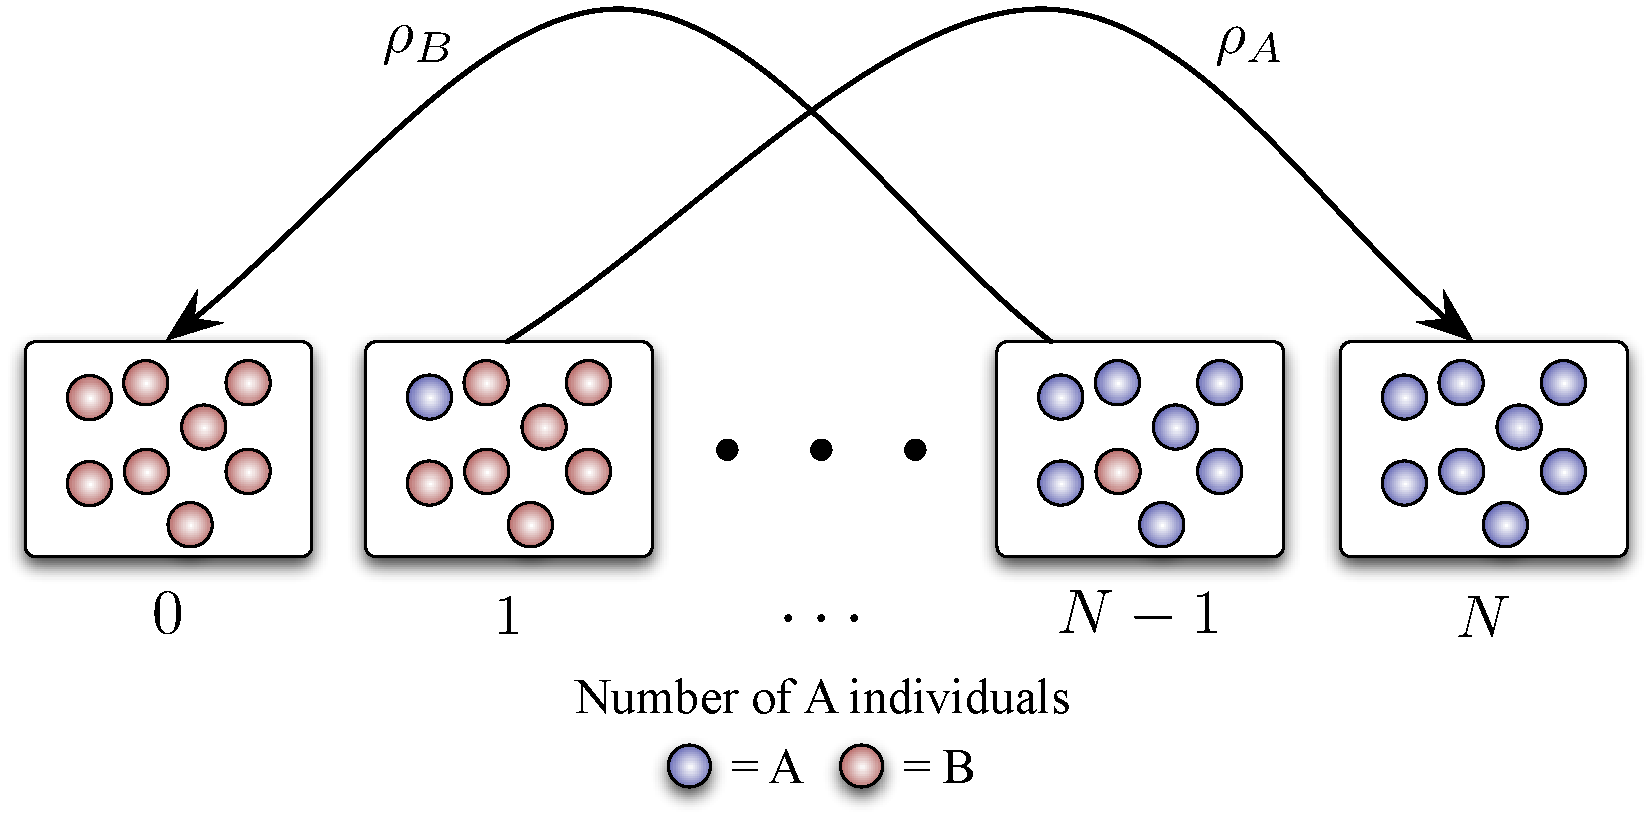
\includegraphics[width=0.7\columnwidth]{fixprob}}
  \end{center}
  \caption{
  \label{fig:fixprob}
  \textbf{Fixation probabilities.}
\small{The probability that a single $A$ individual will take over the whole population is known as the fixation probability of $A$ given by $\rho_A$.
Similarly we can calculate the fixation probability of a single $B$ individual in a population of $N-1$ $A$ individuals as $\rho_B$.
If the two strategies are neutral with respect to each other then these fixation probabilities are just $1/N$.}
  }
\end{figure}
%

\subsection{One Third Rule}
\label{subsec:OTR}
\index{stochastic processes!one-third rule}
A strategy being favoured by selection means that the fixation probability is greater than neutral.
Considering strategy $A$ that means we need to check if,
%
\begin{eqnarray}
\rho_A > \frac{1}{N}.
\end{eqnarray}
%
For weak selection the product in the fixation probability can be approximated by a sum,\index{stochastic processes!fixation probability}
%
\begin{eqnarray}
\rho_A \approx \frac{1}{N}+\frac{w}{N^2}\underbrace{\sum_{m=1}^{N-1}\sum_{j=1}^{m}\left( \pi_A - \pi_B \right)}_{\Gamma}.
\end{eqnarray}
%
It is then apparent that for $\rho_A > 1/N$, $\Gamma$ should be greater than zero.
That is,
%
\begin{equation}
\sum_{m=1}^{N-1}\sum_{i=1}^{m} \pi_A > \sum_{m=1}^{N-1}\sum_{i=1}^{m}\pi_B. \nonumber
\end{equation}
%
Substituting the values of $\pi_A$ and $\pi_B$ from Eqs.\ \eqref{finitepayoffs},
\begin{equation}
\sum_{m=1}^{N-1}\sum_{i=1}^{m} \left(\frac{i-1}{N-1} a_1 + \frac{N-i}{N-1} a_0\right) > \sum_{m=1}^{N-1}\sum_{i=1}^{m} \left(\frac{i}{N-1} b_1 + \frac{N-i-1}{N-1} b_0 \right). \nonumber \\
\end{equation}
This can be simplified to,
\begin{equation}
a_1 (N-2) + a_0 (2 N -1) > b_1 (N+1) + 2 b_0 (N-2).
\label{finite13rd}
\end{equation}
%
We thus arrive at Inequality \ref{finite13rd} which is the condition in finite populations and depending only on the relationship between payoff values.
For a large $N$this reduces to $a_1 +2 a_0 > b_1 + 2 b_0$, which is equivalent to,
%
\begin{eqnarray}
\frac{1}{3} &>& \frac{b_0 -a_0}{a_1 - a_0 - b_1 + b_0} = x^*,
\end{eqnarray}
%
calculated as the position of the possible internal equilibrium in Eq.\ \eqref{inteq}.
The internal equilibrium $x^*$ can be in the interior if $a_1 > b_1$ and $a_0<b_0$ (a bi-stability game) or if $a_1 < b_1$ and $a_0>b_0$ (a co-existence game).
The condition means that if a strategy at frequency \textit{one third} has a fitness greater than the fitness of the other strategy then the fixation probability of that strategy is greater than neutral.
This special relation between the internal equilibrium and the condition for a strategy to have a fixation probability greater than neutrality is termed as the one-third rule \citep{ nowak:2004pw,traulsen:2006bb,imhof:2006aa,ohtsuki:2007aa,bomze:2008lr}.\index{Kingman, J.F.C.!coalescence theory}
This rule is valid for all process which fall in the domain of Kingman's coalescence \citep{lessard:2007aa}


\subsection{Risk Dominance}
\label{subsec:RD}
\index{stochastic processes!risk dominance}
Having $\rho_A > 1/N$ means that the fixation probability of $A$ is greater than neutral.
As $A$ approaches fixation at some time point we have $N-1$ $A$ individuals and $1$ $B$ individual.
Now if $\rho_B > 1/N$ then the fixation probability of $B$ will be greater than neutral.
Hence it is necessary to determine which strategy has a higher fixation probability.
Usually we ignore mutations between strategies.
Selection and mutations work in tandem and maintain the population at the mutation selection equilibrium but if the mutation rate is very low then we can calculate the approximate stationary distribution by using the fixations probabilities as a proxy.
In short we want to know which strategy is more likely to replace the other.
Using Eqs.\ \eqref{rhoa} and \eqref{rhob} we get,
%
\begin{eqnarray}
\frac{\rho_B}{\rho_A} &=& \prod_{i=1}^{N-1} \frac{T_i^-}{T_i^+}.
\label{eq:fpratio}
\end{eqnarray}
%
Let the ratio of transition probabilities be $\gamma_i$.\index{stochastic processes!transition probabilities}
Then we have,
%
\begin{eqnarray}
\gamma_i = \frac{T_i^-}{T_i^+} = \frac{f_B}{f_A} =\frac{1 - w + w \pi_B}{1 - w + w \pi_A} \approx 1 - w (\pi_A-\pi_B),
\end{eqnarray}
%
 where we have assumed that selection is very weak that is $w\ll1$.
Substituting in Eq.\ \eqref{eq:fpratio} we get,\index{stochastic processes!fixation probability}
%
\begin{eqnarray}
\frac{\rho_B}{\rho_A} &\approx& \prod_{i=1}^{N-1} 1 - w (\pi_A-\pi_B) \nonumber \\
&=& 1 - w \sum_{i=1}^{N-1} (\pi_A-\pi_B) \nonumber.
\end{eqnarray}
%
Substituting the values of $\pi_A$ and $\pi_B$ from Eqs.\ \eqref{finitepayoffs},
%
\begin{eqnarray}
\frac{\rho_B}{\rho_A} &\approx& 1 - w \underbrace{\sum_{i=1}^{N-1} \left(\frac{i-1}{N-1} a_1 + \frac{N-i}{N-1} a_0 - \frac{i}{N-1} b_1 - \frac{N-i-1}{N-1} b_0\right)}_{\Phi} \nonumber.
\end{eqnarray}
%
Hence we have $\rho_A > \rho_B$ if $\Phi > 0$ which reduces to,
%
\begin{equation}
N (a_0+a_1) - 2 a_1 > N (b_0+ b_1)-2 b_0.
\end{equation}
%
This result holds for a large number of birth-death processes for weak selection \citep{nowak:2004pw,antal:2009th}
and also for some special processes at any intensity of selection \citep{antal:2009th}.
In the limit of a large population size we can ignore the terms without $N$ and thus get,
%
\begin{equation}
\label{rdcond}
a_1+a_0 > b_1 + b_0
\end{equation}
%
Thus if the above inequality is fulfilled then for a large population under weak selection, strategy $A$ will have a higher fixation probability than strategy $B$.
This condition is also known as risk dominance \citep{harsanyi:1988mm,kandori:1993aa}.
Intuitively risk dominant strategy is the one which you choose if you have no information about your opponent's strategy.
In other words it just means knowing which is your safest bet.

%%%%%%%%%%%% use the following when including the page number of two sided print
%\newpage
%qw
%\newpage
%---------------------------------------------EGTMultiverse-------------------------------------------------

\begin{savequote}[10pc]
\sffamily
``\ldots human life is a many-person game and not just a disjoined collection of two-person games"
\qauthor{William D. Hamilton ($\oldstylenums{1936}-\oldstylenums{2000}$)}
\end{savequote}

\chapter{Evolution in the multiverse}
\label{chap:multiverse}

\graphicspath{{Figs_Multiverse/}{Figs_Multiverse/}{Figs_Multiverse/}}

\section{Evolutionary games in the multiverse}
\label{sec:multiverse}

\citet{stander:1992aa} has described the hunting behaviour of lionesses on the open semi-arid plains of Namibia.\index{lions!group hunting}\index{lions!Etosha National Park}
Individual hunting tactics of lionesses were analysed from $486$ independent group hunts.
The lionesses hunt in packs and employ the flush and ambush technique (see Fig.\ \ref{fig:stander}).
Some lie in ambush while others flush out the prey from the flanks and drive them towards the ones waiting in ambush.
This technique needs an interaction of more than two players to succeed.

Similarly, we interact with innumerable people at the same time, directly or indirectly. 
Some interactions may be pair-wise, but others are not.
In real life, we may typically be engaged in many person games instead of a disjoined collection of two person games \citep{hamilton:1975aa}.
%
\begin{figure}[h]
  \begin{center}
    \leavevmode
    \boxed{ 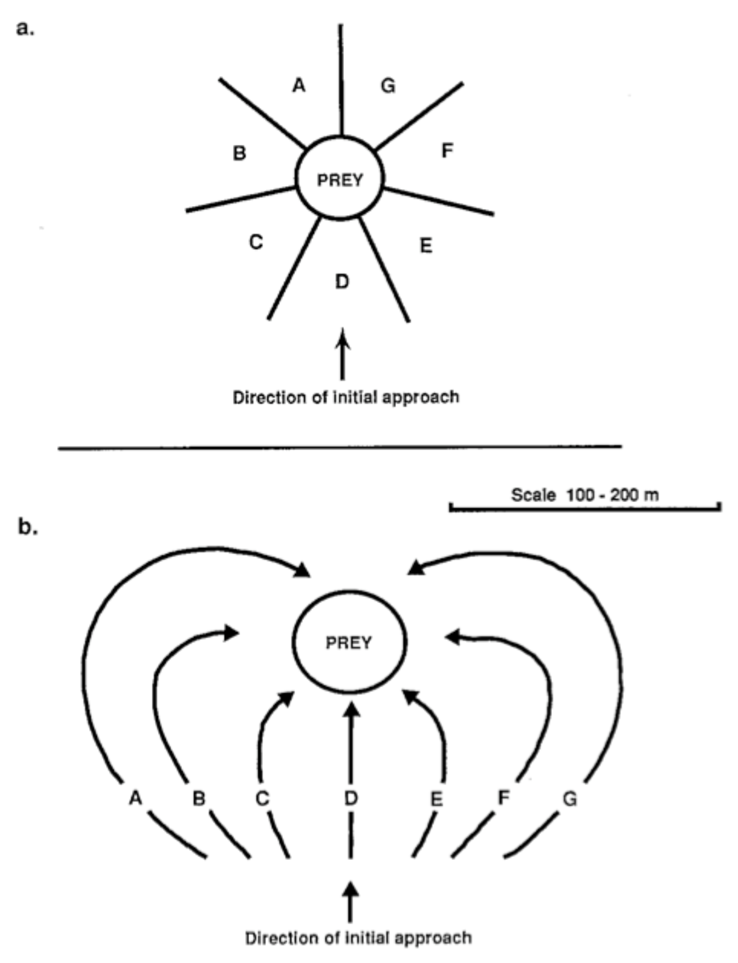
\includegraphics[width=0.45\columnwidth]{stander}}
    \caption{\textbf{Flush and Ambush.}
    \small{Taken from \citet{stander:1992aa} this sketch describes the flush and ambush technique used by the lionesses in Etosha National Park.
    Top panel reflects the position of the lionesses from the point of view of the prey.
    The bottom panel shows the attack positions of the lionesses. $A-B$ form the left flank while $F-G$ are the right flank.
    $C-D-E$ take the centre position. This hunting set-up is not possible with just two lionesses.}
    }
    \label{fig:stander}
  \end{center}
\end{figure}
%
Evolutionary game theory which we have discussed until now has been about two player games.
It becomes mathematically more demanding when we try to include more players.
\citet{hamilton:1975aa} illustrates the theoretical challenges of multiplayer games as, 
\textit{``The theory of many-person games may seem to stand to that of two-person games in the relation of sea-sickness to a headache."}
A special class of multiplayer games has been experimentally and theoretically studied by economists and sociologists to study social behaviour of individuals.
Such a typical ``public goods game" consists of participants who have an option of contributing to a common pot.
The sum is shared equally amongst all participants. 
Numerous variants of this basic set-up have been explored \citep{wedekind:2000gw,milinski:2001og,anderson:2001aa,hauert:2002te,semmann:2003he,milinski:2006aa,rockenbach:2006aa,hauert:2007aa,milinski:2008lr,santos:2008xr,pacheco:2009aa,souza:2009aa,veelen:2009ma,traulsen:2010pn,connor:2010aa}.\index{multiple strategies}
We develop some general conditions for multiplayer games with multiple strategies with simplicity in mind \citep{kurokawa:2009aa,gokhale:2010pn}.
To refrain from repeating the word ``multi" for player and strategies we use the short form ``games in the multiverse" for these kind of games.

Let us begin with the well known scenario of two player games with two strategies and add one more player to this setting.
The changes which happen are reviewed below,

\begin{itemize}
\item The payoff matrix for a $2 \times 2$ games is a square matrix whereas for a $2 \times 2 \times 2$ player game it is an extended table of permutations (see Fig.\ \ref{fig:general2by2by2}).
\item The dynamics for a $2 \times 2$ proceeds on a simplex which is one dimensional, a single line.
	Even for $2 \times 2 \times 2$ games there are only two strategies and thus the simplex is a single line.
\item There are five possible outcomes for a $2 \times 2$ game, as shown in Fig.\ \ref{fig:general2by2by2}.
As the number of player increases the possible internal equilibrium points also increase.
For $2 \times 2 \times 2$ games all the scenarios from $2 \times 2$ games are possible and in addition there is a possibility of having two equilibria in the interior, one stable one unstable (see Fig.\ \ref{fig:general2by2by2}).
\end{itemize}
%
Adding a player to the usual setting increases the complexity.
The level of complexity increases as more and more players are added.\index{multiple players}
In this project we examine this complexity and extract simple relations from it.
%
\begin{figure}[!h]
  \begin{center}
\boxed{ 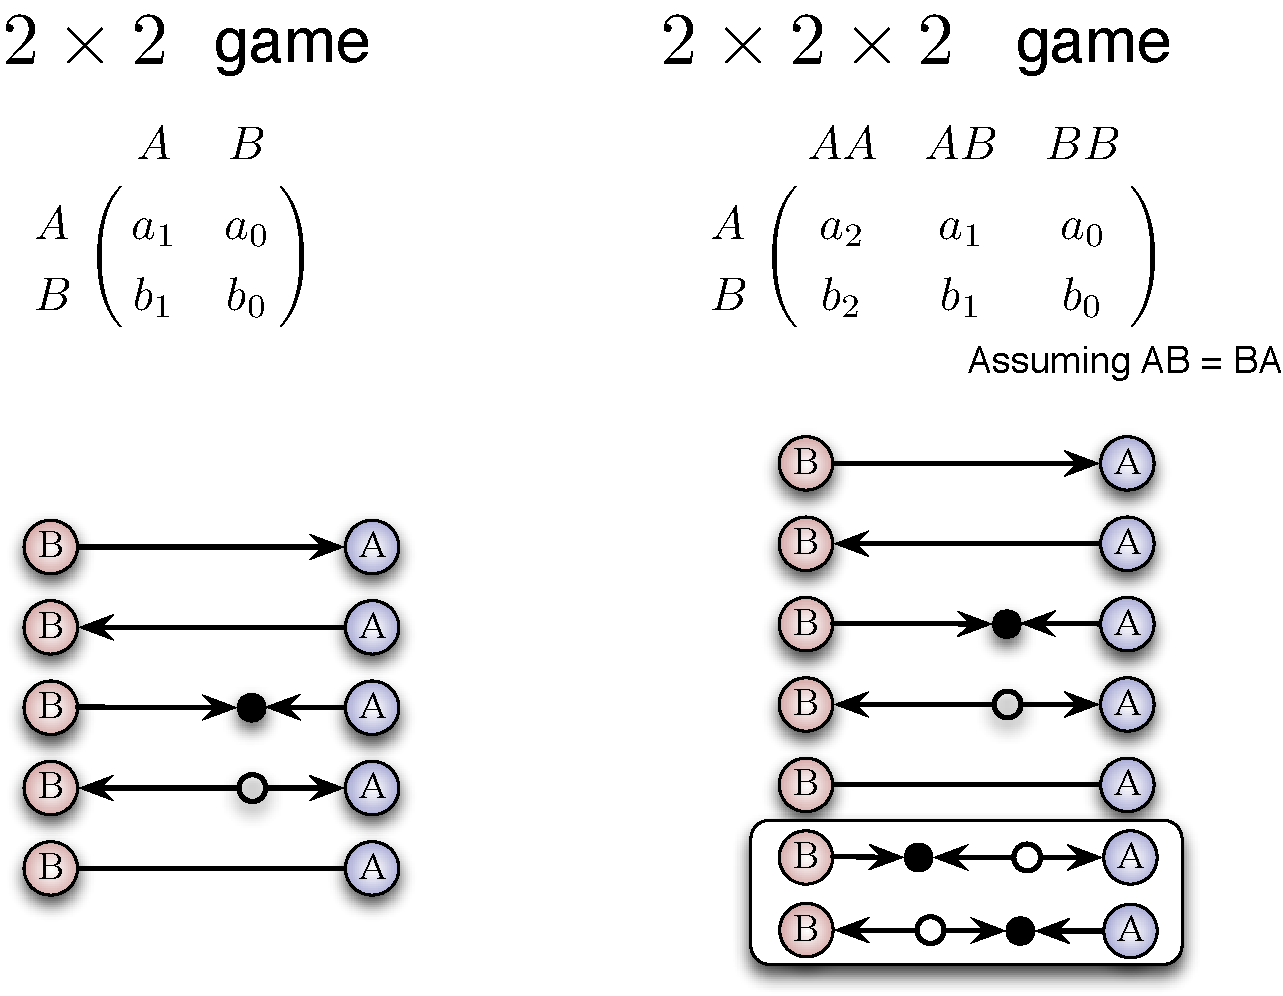
\includegraphics[width=0.7\columnwidth]{general2by2by2}}
    \caption{\textbf{Comparing two player games with three player games for two strategies.}
   \small{Writing the payoffs for three player games cannot be done in a square payoff matrix as two player games.
   Instead it is a table of permutations of a player playing with $2$ other players.
   For two player games there are five possible outcomes.
   As the payoffs are linear in $x$ there can be at most a single internal equilibrium.
   For three player games the payoffs are not linear in $x$ but of degree $2$ leading to at most two possible solutions in the interior of the simplex.}}
    \label{fig:general2by2by2}
  \end{center}
\end{figure}
%

There were two main analytical advances in evolutionary game theory in the study of finite populations
for two player games with two strategies.
%
\begin{enumerate}
\item When is the fixation probability of a strategy is greater than neutral (One Third rule) (Sub-section \ref{subsec:OTR})\index{stochastic processes!one-third rule}?
\item When is the fixation probability of a strategy is greater than the fixation probability of the other strategy (Risk Dominance) (Sub-section \ref{subsec:RD})?\index{stochastic processes!risk dominance}
\end{enumerate}
%
We develop general conditions for multiplayer games and two strategies without compromising on simplicity.
Using the infinite population size assumption we also calculate the maximum number of internal equilibria of a given game with multiple player and multiple strategies.
%The calculation is inspired from old algebraic manipulations discussed first in \citet{chrystal:1889bo}.

\newpage
\subsection{Publication: Evolutionary games in the multiverse}

Chaitanya S. Gokhale, Arne Traulsen,\\
Proceedings of the National Academy of Sciences, USA\\
March $23$, $2010$\\
Volume. $107$ Number. $12$\\
Pages $5500-5504$

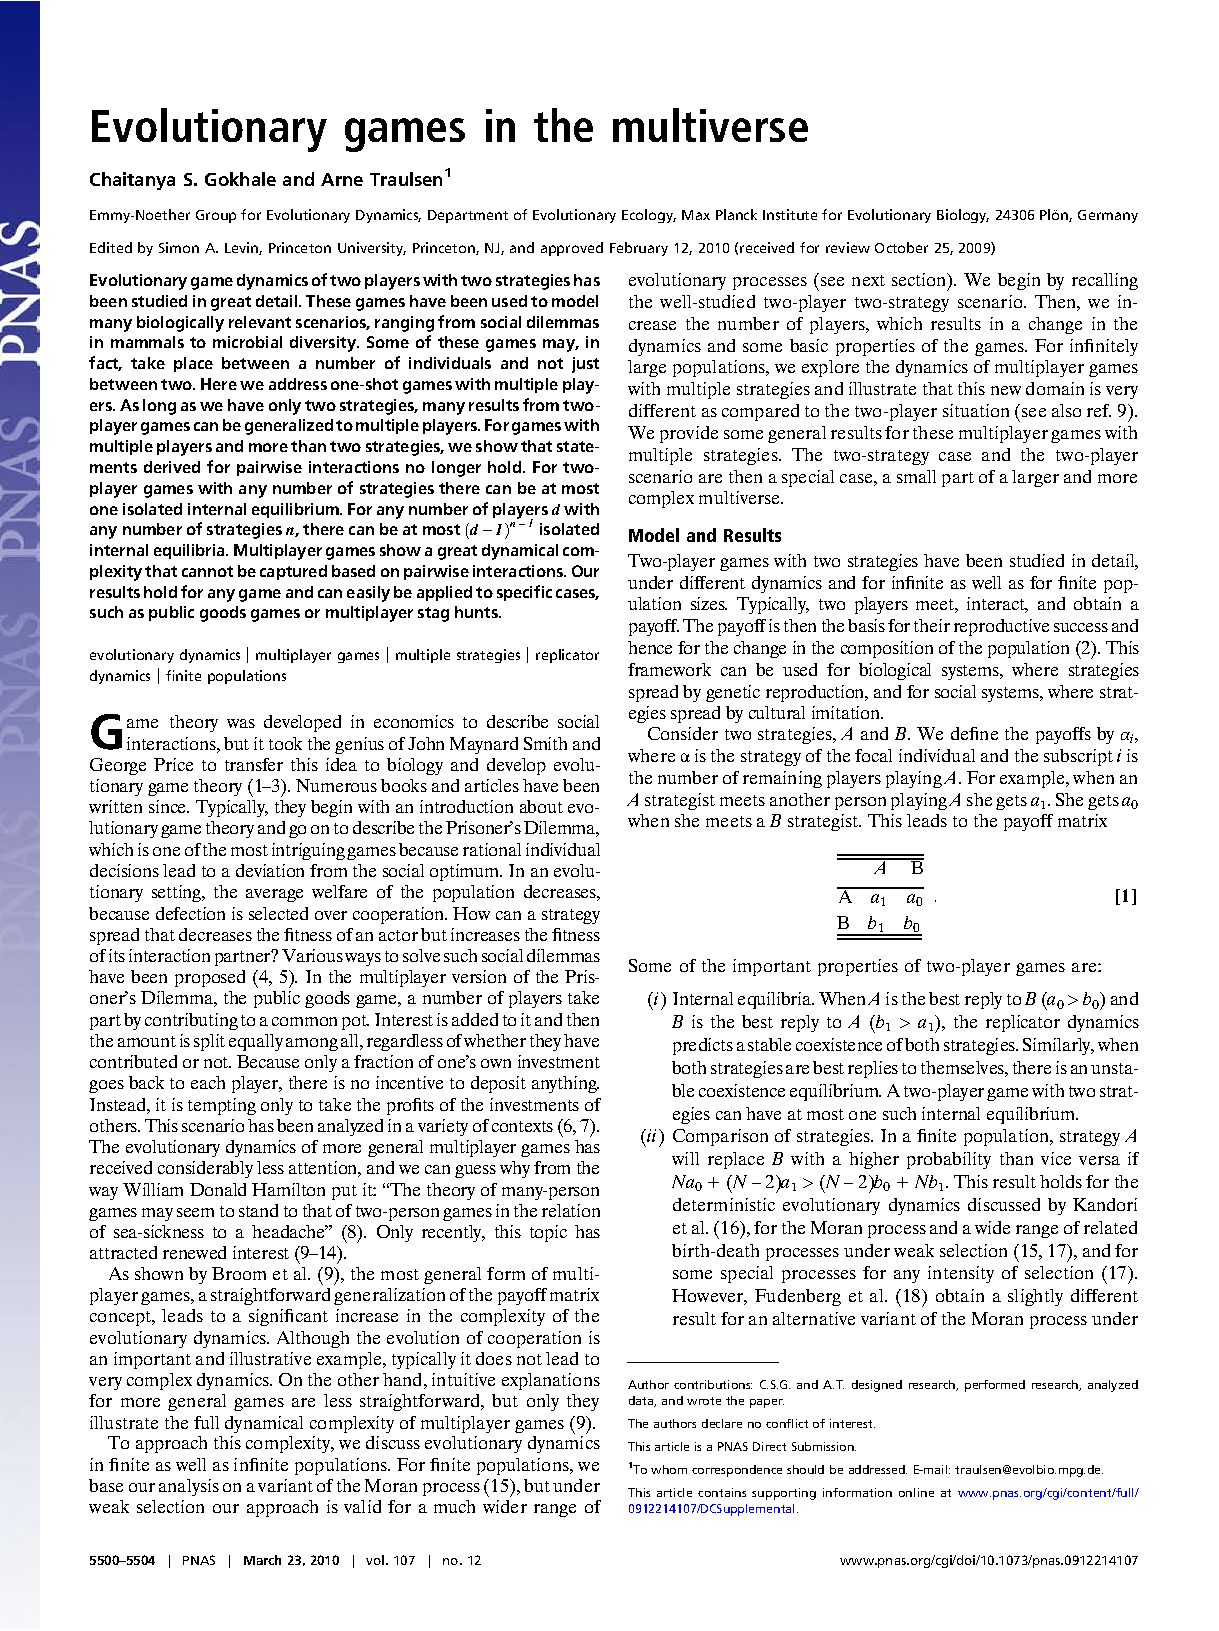
\includepdf[pages=-,scale=0.8]{Papers/Gokhale_PNAS_2010all.pdf}


%---------------------------------------------Small mutation rates-------------------------------------------------

\section{The assumption of ``small" mutation rates}
\label{sec:wgt}

\graphicspath{{Figs_WGT/}{Figs_WGT/}{Figs_WGT/}}

Until now we dealt with selection.
Now in this project, we incorporate mutations as well.
Mutations or random explorations seem to be inherent in human nature.
Mutations and selection work in concert to develop the population to a possible equilibrium state.
Traditionally analyzing multiplayer games with mutations is possible if we assume the mutation rate to be negligible \citep{fudenberg:2008je}.
Consider the situation when we have three strategies $A$, $B$ and $C$.
Every time a reproductive event occurs, there is a small probability $\mu$ that the offspring will be of a random strategy and not necessarily like the parent.
The average time between two mutations is thus $\mu^{-1}$.
We also know that the time for fixation of a single neutral mutant is $N (N-1)$ \citep{antal:2006aa}.
Therefore if the mutation probability, $\mu$, is much smaller than $N^{-2}$ then the time between two mutations will be much larger than the time required for either extinction or fixation of a single mutant.
Thus at a time we will have to deal with only two strategies.
For two strategies we can calculate exactly the fixation probability of a mutant in finite populations \citep{nowak:2006bo} even for multiplayer games \citep{gokhale:2010pn}.
For small mutation rates the transition probabilities between different strategies consist of just the fixation probabilities.
For example for the three strategies $A$, $B$ and $C$ the transition matrix, $\mathbf{T}$ looks like,
%
\begin{align}
\mathbf{T}=
\bordermatrix{
&&&\cr
& 1-\rho_{AB}-\rho_{AC} & \rho_{AB} & \rho_{AC} \cr
& \rho_{BA} & 1-\rho_{BA}-\rho_{BC} & \rho_{BC} \cr
& \rho_{CA} & \rho_{CB} & 1-\rho_{CA}-\rho_{CB} \cr}
\end{align}
%
where the fixation probability of strategy $A$ in a population consisting predominantly of strategy $B$ is given by $\rho_{AB}$.
Each element of the matrix denotes the probability of the row strategy to move into the column strategy.
Strategy $A$ (first row) can either stay in an all $A$ population (first column) or move to a population of $B$ (second column) individuals or in a population of $C$ (third column) individuals.
Since these are the only three probable events, the sum of all elements in a row is one.
To find which strategy does the best at the mutation selection equilibrium we need to know which strategy has the highest frequency on an average in the stationary distribution.
The stationary distribution of the system is given by the normalised right eigenvector for the largest eigenvalue of the transition matrix $\mathbf{T}$.
However this analysis is only valid for small mutation rates.
The question asked in this section is,
\begin{enumerate}[-]
\item How small do the mutation rates have to be so that the error due to the approximation is below a tolerable threshold?
\end{enumerate}

This issue was can be tackled by using time scale separation analysis based on \citet{antal:2006aa}.
Since then this approach has been used extensively in many papers to explore the the dynamics of strategies in the limit of strong selection and weak mutations \citep{imhof:2005oz,fudenberg:2006ee,traulsen:2007bb,hauert:2007aa,hauert:2008bb,van-segbroeck:2009mi,sigmund:2010aa}.
Our approach takes the route of the stationary distribution.
If we let the system evolve for a long time it will reach an equilibrium state such that we can denote it by a distribution of the frequencies of the different strategies.
For small mutation rates this distribution is approximated by the ones based on the fixation probabilities.
We check for the difference between these two distributions.
To check mathematically if the approximation is ``good" we calculate the total variation distance between the distributions.% calculated by the $p$ norm.

Herein we also provide a numerically accessible bound which can be calculated for any given system of two player games and two strategies.
Hence now it is possible to determine exactly how low the mutation rate should be to reduce the error below a certain threshold.

\subsection{Publication: How small are small mutation rates?}

Bin Wu, Chaitanya S. Gokhale, Long Wang, Arne Traulsen\\
\textit{Journal of Mathematical Biology, In revision}
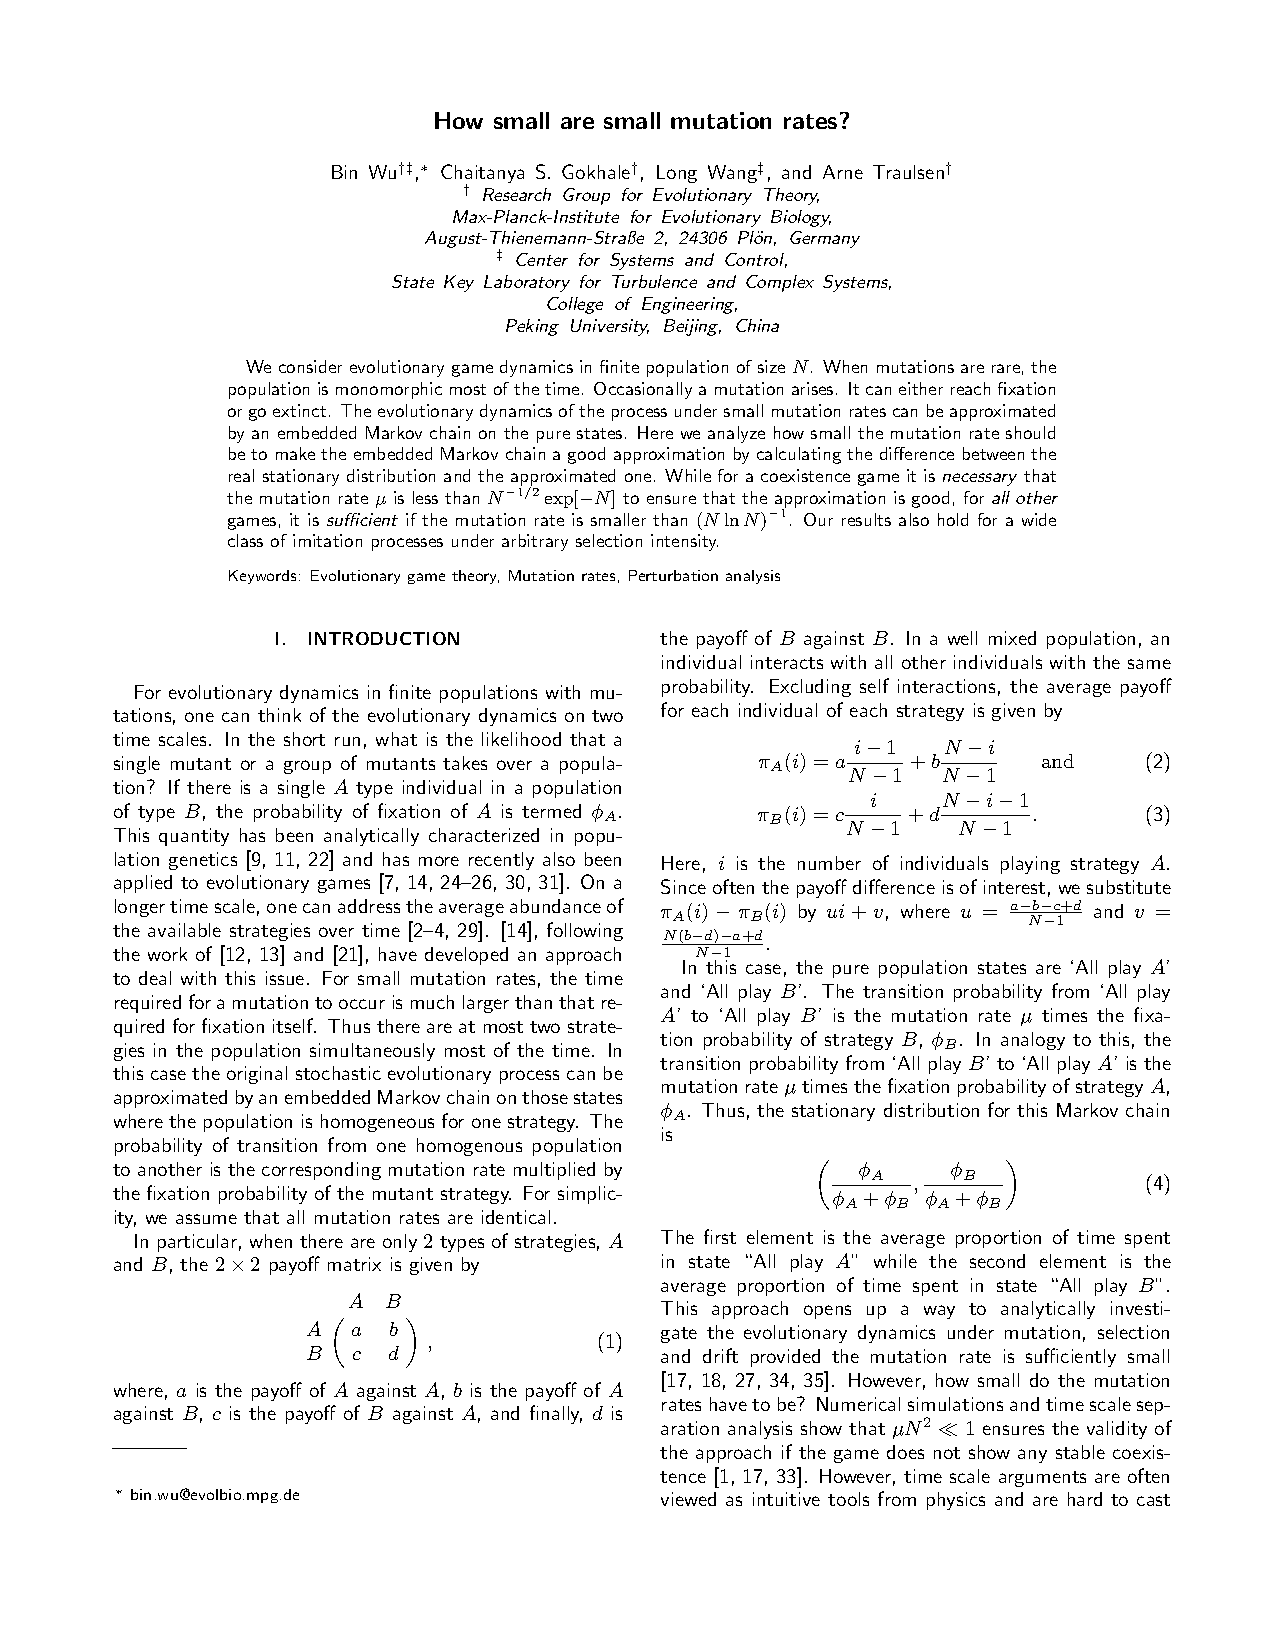
\includepdf[pages=-,scale=0.8]{Papers/Wu_JMBsub_arxiv.pdf}


\section{Mutation selection equilibrium in evolutionary games.}
\label{sec:equilibrium}

\graphicspath{{Mu-Se/}{Mu-Se/}{Mu-Se/}}
\index{mutation selection equilibrium}

Multiplayer games are the representations of many social dilemmas.\index{multiple players}
Even for multiplayer games we can use the replicator equation with a complicated payoff structure to derive the time evolution of the strategies.
This includes only the effect of selection.
Including mutations in a given evolutionary game is relatively easy if we assume the mutation rate to be very small.
This allows us to derive important quantities such as fixation probabilities with relative mathematical ease.
For high mutation rates the concept of fixation itself becomes problematic and so does fixation probability.
Even with high mutation rates, if a system continues to evolve for a long time then we can calculate the average frequency of a strategy.
This average frequency of a strategy in the stationary distribution (hereafter termed as abundance) for arbitrary mutation rates has been calculated previously by \citet{antal:2009th,antal:2009aa,antal:2009hc}.
The procedure can even be applied in some cases when a population is structured \citep{tarnita:2009jx}.
The analysis has remained possible only for two player games.

We develop an approach for estimating the abundance for multiple players and multiple strategies..
The theory hinges on the calculation of the following term, the average change in the frequency of strategy $k$ under weak selection ($\delta \ll1$),
%
\begin{equation}
\langle \Delta x_k^{sel} \rangle_\delta. \nonumber
\end{equation}
%
Once we know this then we can add the effect of mutations ($u$) which gives us the abundance of a strategy (here strategy $k$) in the mutation-selection equilibrium \citep{antal:2009th,antal:2009aa,antal:2009hc} as,
%
\begin{equation}
\langle x_k \rangle_\delta = \frac{1}{n} + N \frac{1-u}{u} \langle \Delta x^{sel}_k \rangle_\delta
\end{equation}
%
For the calculations we employ tools from coalescence theory \citep{kingman:1982aa,kingman:1982bb,kingman:1982cc,kingman:2000fk,wakeley:2008aa}.\index{Kingman, J.F.C.!coalescence theory}
Small mutation rates make sense in genetical sense but for cultural traits such as fashion or plastic behaviour, high mutation rates are more realistic \citep{traulsen:2010pn,grujic:2010aa}.
The theory developed herein can be used for a variety of applications ranging from finding the abundance of alleles in an allelic polymorphism to the best strategy in a social setting.
%
\begin{figure}[!h]
  \begin{center}
    \leavevmode
      \boxed{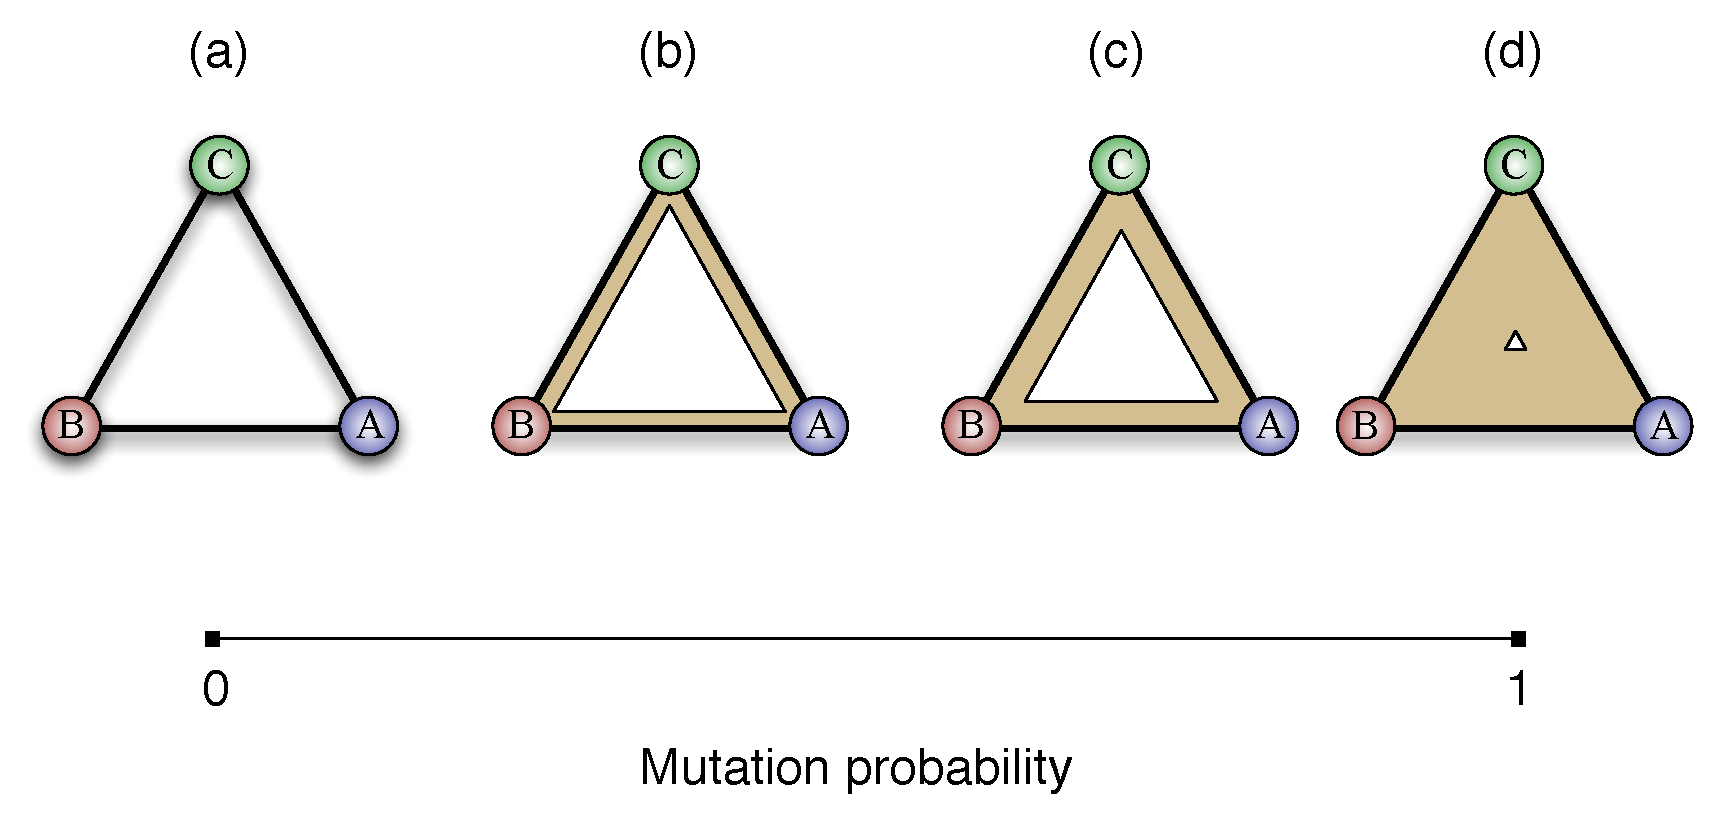
\includegraphics[scale=0.3]{mutsimplices}}
    \caption{\textbf{Available space in the simplex with increasing mutation probability.}
    \small{In infinitely large populations as mutation probability increases, the area where a stable coexistence is possible decreases.
    (a) If a population is at a certain homogeneous state, all $A$, all $B$ or all $C$ then it will stay there forever.
For very low mutation rate if a system is in a homogeneous state then occasionally a mutant arises and the edges of the simplex are explored.
(b) For sufficiently high mutation rates the system leaves the edges. the possible space for a stable coexistence becomes constricted (white interior).
(c) As mutation probability increases the system is driven towards a state of eternal heterogeneity where all strategies coexist.
(d) For a mutation probability of $1$ all three strategies coexist at equal frequencies in the center of the simplex at $\left(\frac{1}{3},\frac{1}{3},\frac{1}{3}\right)$.
}}
    \label{mutsimplices}
  \end{center}
\end{figure}
%


\subsection{Publication: Mutation selection equilibrium in multiplayer games with multiple strategies}

Chaitanya S. Gokhale, Arne Traulsen,\\
\textit{Submitted}
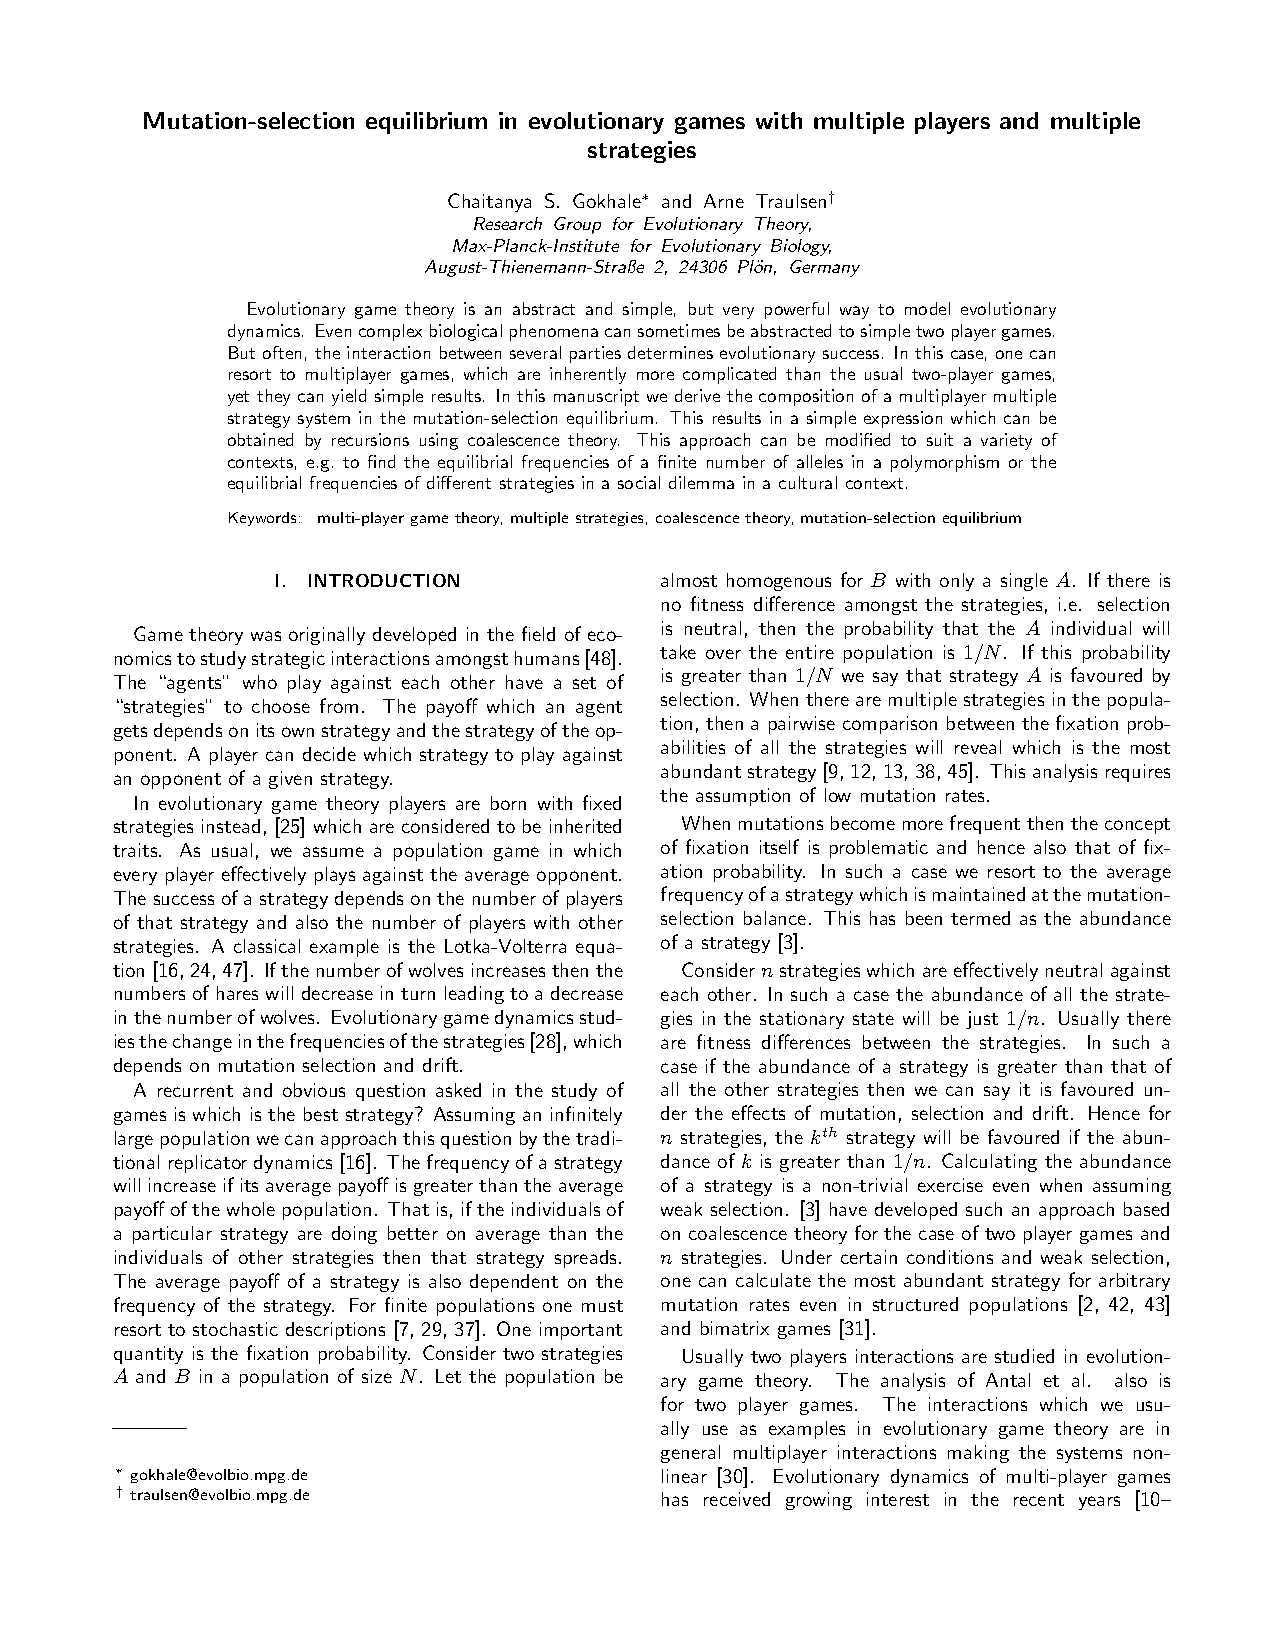
\includepdf[pages=-,scale=0.8]{Papers/Gokhale_JTBsub_arxiv.pdf}

%-----------------------Medea-----------------


\section{Evolutionary games and Medea allele dynamics}
\label{chap:medea}
\graphicspath{{Figs_Medea/}{Figs_Medea/}{Figs_Medea/}}

The previous publications in this thesis dealt with extending the theoretical limits of frequency independent and frequency dependent models of evolution.
This publication stands apart as it is an application of the theories developed so far.
Herein, evolutionary game theoretic arguments are employed to 
\begin{enumerate}
\item show how the dynamics of the Medea alleles can be used to an advantage in genetic pest management techniques and 
\item explain the evolution of natural Medea elements.
\end{enumerate}
\textbf{\underline{M}}aternal \underline{\textbf{e}}ffect \underline{\textbf{d}}ominant \underline{\textbf{e}}mbryonic \underline{\textbf{a}}rrest (Medea) is a selfish gene \citep{hurst:1996aa,hurst:2001gg}.
It was first discovered in \textit{Tribolium} flour beetles \citep{beeman:1992aa}.\index{\textit{Tribolium}}
The Medea allele increases in frequency at the cost of the wildtype allele.\index{Medea}
The effect of the Medea allele can be seen if the mating involves a female heterozygous for Medea.
%
\begin{figure}[h]
  \begin{center}
    \leavevmode
      \boxed{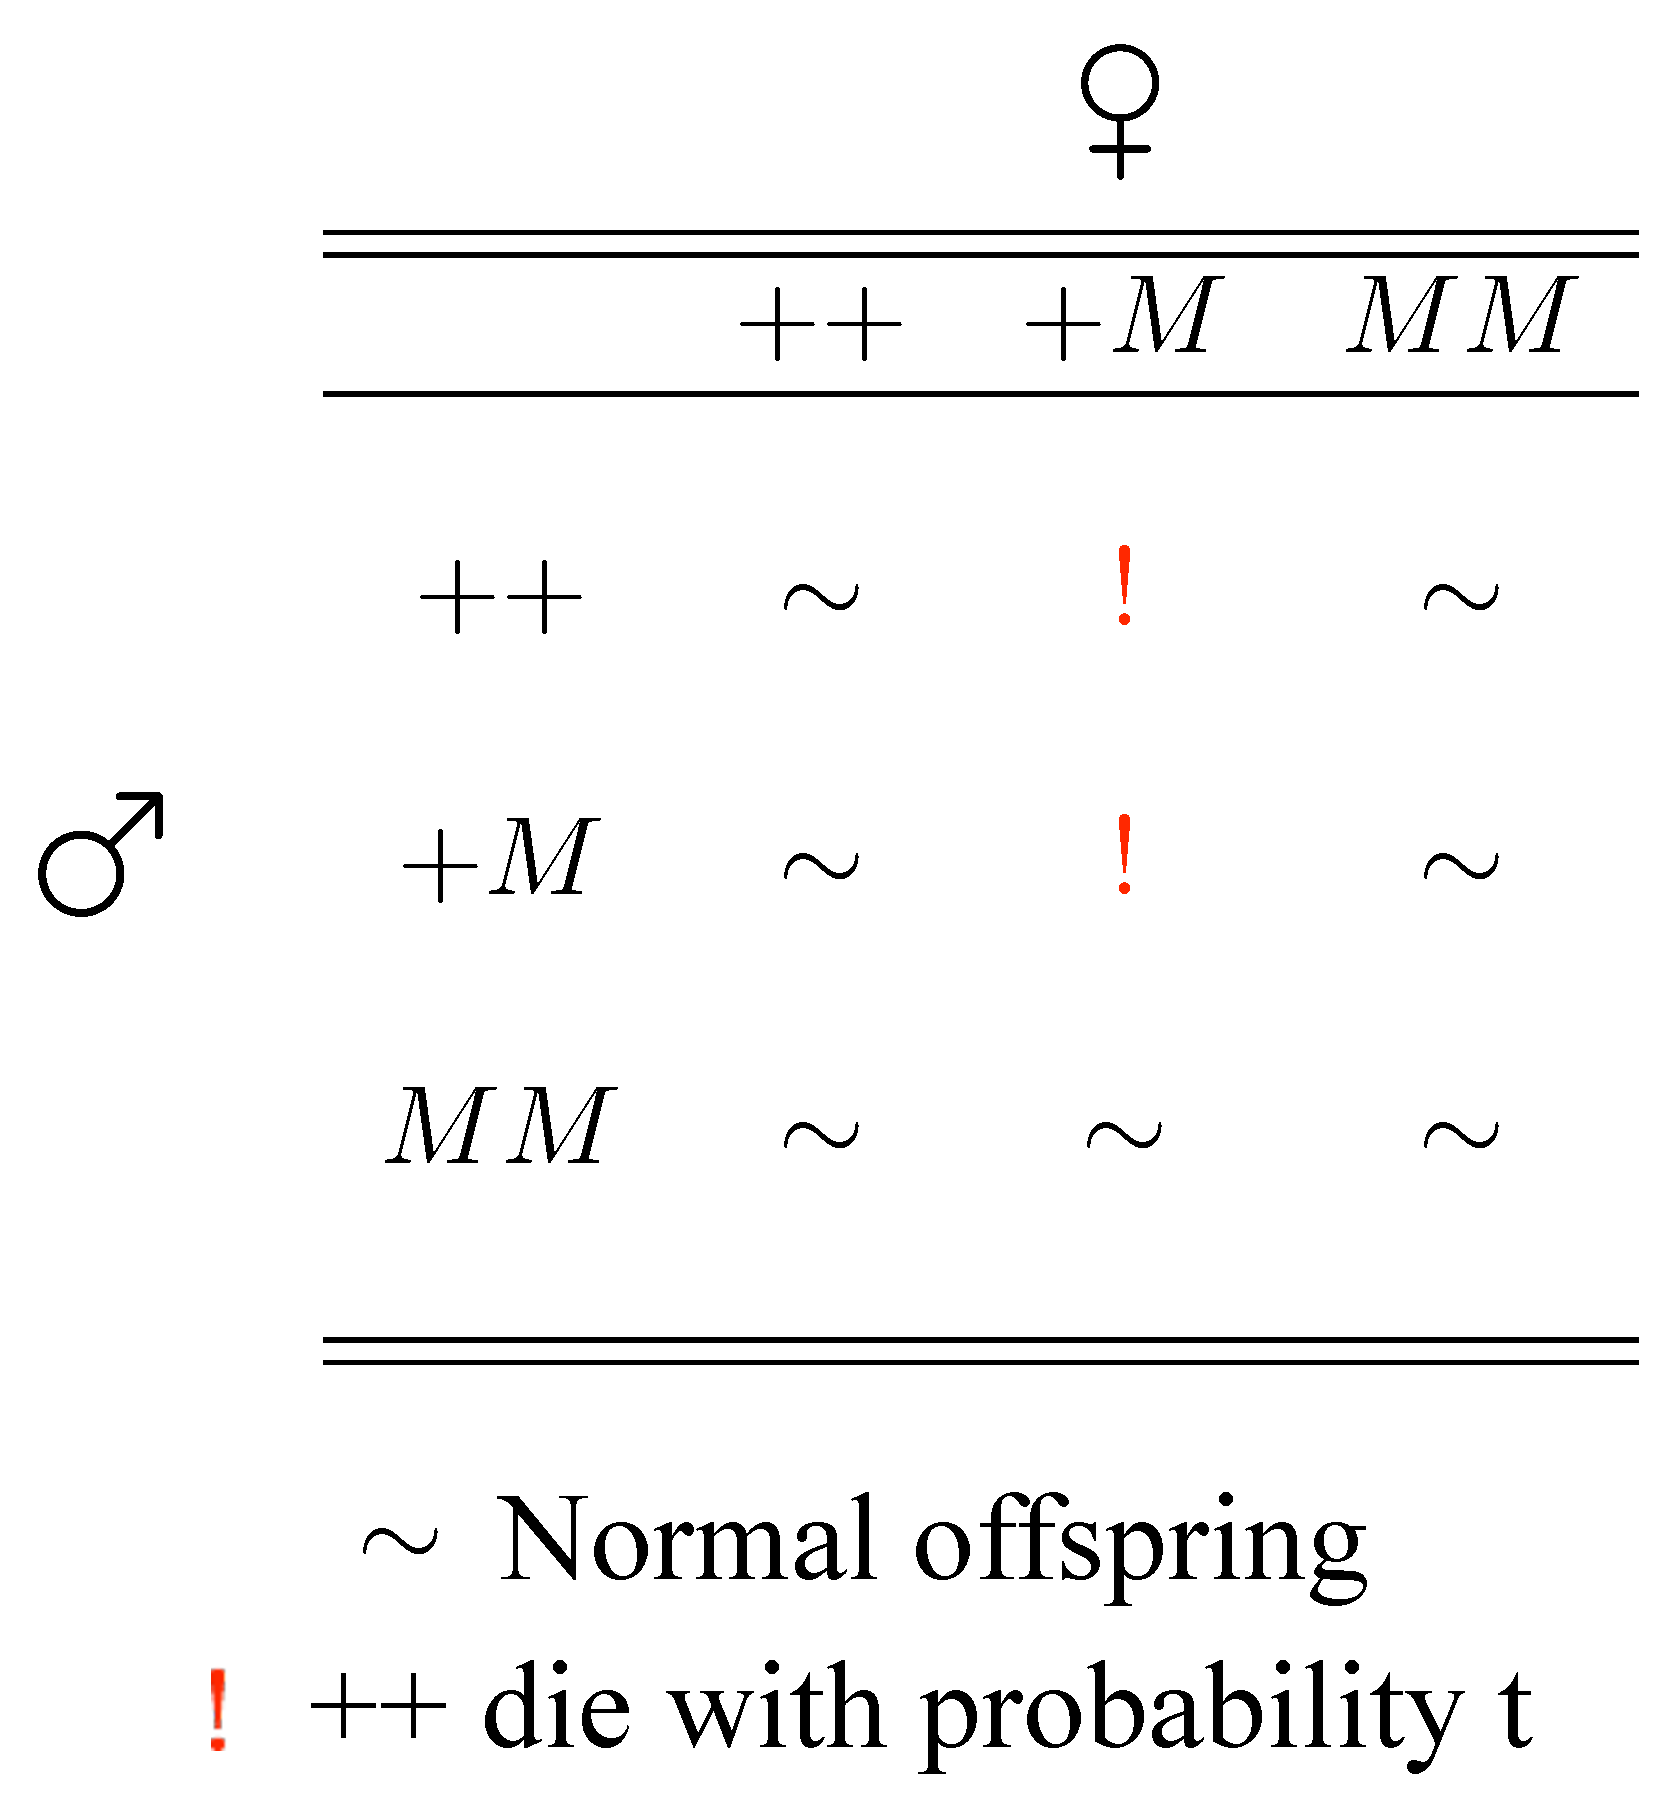
\includegraphics[scale=0.2]{medeasystem}}
    \caption{\textbf{Effect of the Medea allele is seen in offsprings when mothers are heterozygous for Medea.}
    \small{If the mother is a Medea carrier then she deposits a poison in the germline.
    Only the offspring who have a copy of the Medea allele can produce the antidote and can survive.
    Thus the wild-type homozygous offspring of heterozygote parents or of heterozygote mother and wild-type homozygous father are affected.}
}
    \label{fig:medeasystem}
  \end{center}
\end{figure}
%
The Medea system works by producing a ``poison" and a ``rescue".
Females possessing a Medea allele deposit the ``poison" in the germline.
If the resulting zygotes do not contain an endogenous rescue then they do not survive; in effect heterozygous (carrier) mothers can effectively kill off their homozygous wildtype offspring (see Fig.\ \ref{fig:medeasystem}).
Thus, Medea elements can increase in frequency in a population, even if they are not beneficial to the organism \citep{beeman:1992aa,wade:1994aa}.
The dynamics of the Medea allele have been well studied in theory and in the laboratory \citep{wade:1994aa,smith:1998aa}.\index{selfish gene}
These maternal-effect selfish alleles have also been reported in the mouse \citep{peters:1993aa,weichenhan:1996aa}. 

A synthetic Medea system has been engineered in \textit{Drosophila melanogaster} that mimics the natural Medea system and has the same invasive properties \citep{chen:2007aa}.\index{\textit{Drosophila melanogaster}}
It has been proposed as a transformation system to genetically modify wild populations \citep{chen:2007aa}.
Many proposed genetic pest management approaches rely on the introduction of genetic modifications, such as disease resistance in a vector species, using an evolution based population-transformation system.
Gene drive mechanisms, engineered to genetically transform wild populations, are of little use in the real world unless they can be controlled. 
While Medea elements can, in theory, transform populations, they are very difficult to control once spread and can wipe out the resident population.
Here, we describe the predicted properties of a combined system genetically linking a Medea construct with underdominance.\index{underdominance}
Underdominant systems typically require the release of very large numbers of individuals to result in a stable population transformation but are more likely to be spatially contained and, if desired, completely removed from the wild.
When combined with Medea this release threshold can be reduced (see Fig.\ \ref{fig:medeaUD}).
A combination of currently available techniques can results in a system with desirable theoretical properties, which in broad circumstances surpass those of the single systems considered individually.
These enhanced properties include more ideal population transformation thresholds with potential reversibility, mutational stability, and enhanced spatial stability.

In small finite populations Medea elements can invade from very low frequencies with elevated probabilities, even with corresponding fitness costs.\index{stochastic processes}
This has implications for understanding the evolution of natural Medea elements.
%
\begin{figure}[h]
  \begin{center}
    \leavevmode
      \boxed{\includegraphics[width=0.8\columnwidth]{medeaUD}}
    \caption{\textbf{Benefits of a combined Medea-Underdominant system.}
\small{(a) The Medea system by itself allows the selfish gene to sweep through the population.
If the Medea allele has a small cost then the threshold frequency from where it can sweep through the population is very low.
Also due to the cost it will not be able to fix in the population.
(b) Underdominant systems usually have very high natural transformation thresholds and very large releases are necessary to overcome them.
(c) A combination of Medea and underdominance brings together the best features of both the systems.
The high transformation threshold of underdominance is lowered by Medea to practical release frequencies and the Medea element is more controllable.}
}
    \label{fig:medeaUD}
  \end{center}
\end{figure}
%

\subsection{Publication: Dynamics of a linked Medea-Underdominance Population Transformation System}

Chaitanya S. Gokhale, R. Guy Reeves, Floyd A. Reed,\\
\textit{In preparation}
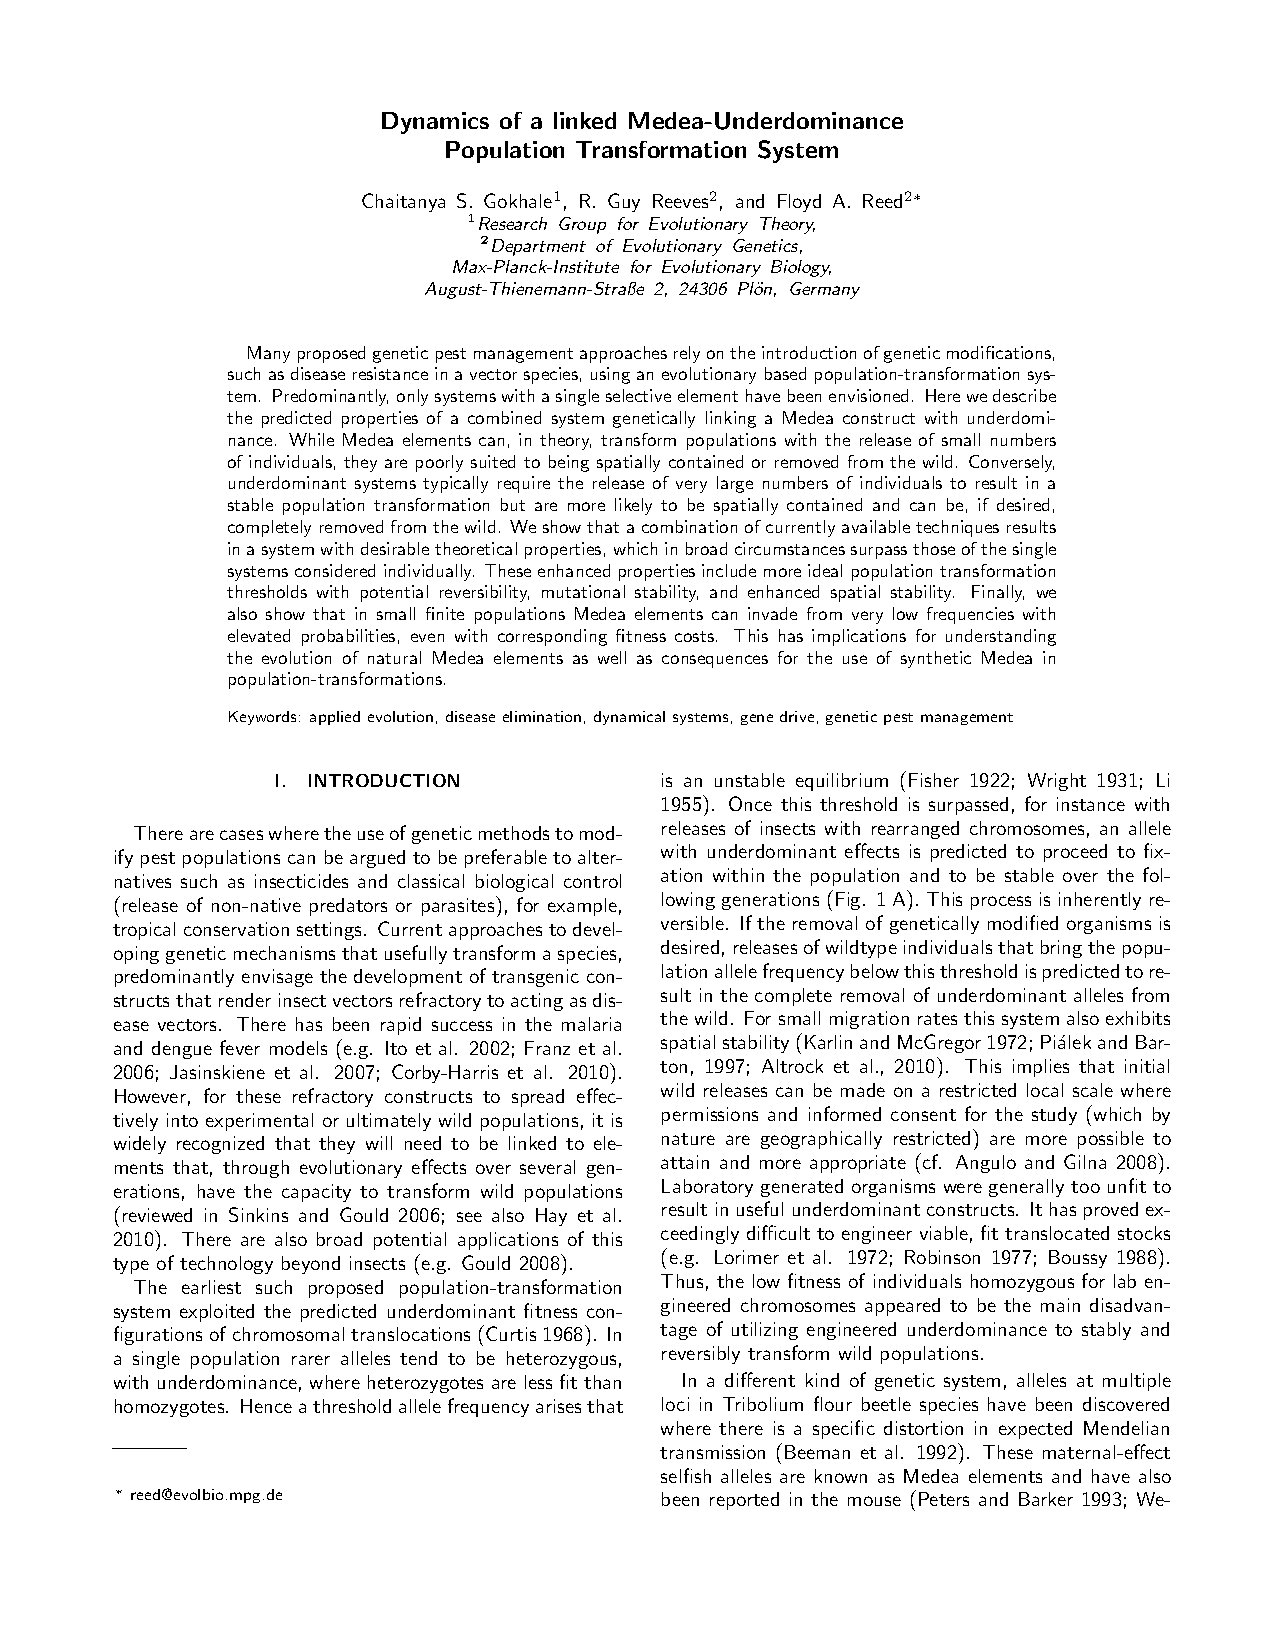
\includepdf[pages=-,scale=0.9]{Papers/Gokhale_Medeasub_arxiv.pdf}

% -------------------------Chapter 4--- Conclusions and Outlook-----------------------------------------------


\begin{savequote}[10pc]
\sffamily
``It is vain to do with more what can be done with fewer."
\qauthor{William of Occham \\
(c.\ $\oldstylenums{1288}$-$\oldstylenums{1348}$)}
\end{savequote}

\def\baselinestretch{1}
\chapter{Summary and Outlook}
\label{chap:conclu}

\graphicspath{{Discussionfigs/}{Discussionfigs/}{Discussionfigs/}}

\def\baselinestretch{1.66}

In the Introduction we mentioned biological systems as complex dynamical systems.
The theory of dynamical systems has its roots in Newtonian mechanics \citep{strogatz:2000bb}.\index{dynamical system!Newtonian mechanics}
In dynamical systems we write down a difference or differential equation which has all the parameters crucial for describing the dynamics of a system.
Depending on the interactions of those parameters the equation gives us the time development of the system.

Analysing evolutionary dynamics in higher dimensions we face the question, is it is really necessary to include all this complexity?
To comment on this question we go through the following argument.
Consider the publications based on static fitness landscapes.
How long does it take for a population to switch peaks if there are two possibilities, a narrow ridge or a broad valley?
A basic requirement of this approach is that there have to be multiple states.
If there were just two states then the question becomes irrelevant.
Multiple states are very realistic for example in cases where fitness is determined by multiple traits.
Accepting this idea, we see that even if one has to go through the valley, it can be faster if there are multiple paths available in it instead of a fixed path with no fitness reduction.\index{fitness!fitness valleys}\index{fitness!fitness landscape}
Next, a peculiar property relating to the time for fixation is studied.
In this case there is no need for multiple states.
The whole study is based on a population moving from state $B$ to $A$ with a slight bias for moving towards $A$.
All else being same if there is a small frequency dependent bias for the population to move from one state to the next then the time for fixation is actually larger than if there is no bias. 
We can extend this knowledge to multiple states and conjecture the following:
Imagine a population moving on a flat landscape.
Even if there is a small bias for moving in a particular direction for each transition, the time required will be greater than neutral and hence in all it will take longer to cross the landscape as compared to a balanced process.

To study frequency dependent scenarios we use evolutionary game theory.
Evolutionary game theory has become quite popular amongst behavioral ecologists, sociologists, philosophers and also back among economists from where game theory originated \citep{hammerstein:2005aa}.
Evolutionary game theory usually deals with two player games with two strategies.
The publications relating to evolutionary game theory, collated, in Chapter \ref{chap:multiverse}, increase the dimensions of analysis by including multiple players and multiple strategies.\index{multiple strategies}\index{multiple players}
Is the analysis of this increased complexity justified?

The evolution and maintenance of co-operation is definitely one of the most active research areas in biology, sociology and economics.\index{co-operation!evolution of}\index{co-operation!maintenance of}
Social dilemmas have been extensively analysed using evolutionary game theory \citep{ostrom:1990bo,nowak:2006pw,taylor:2007bb}.
Using the Prisoners Dilemma and many other such social dilemma games the problem has been tackled both theoretically and experimentally.
At the heart of many of these experiments are problems which involve multiple players.
Multiplayer games span a wide range of topics, worldwide co-operation to combat global warming, inferring social structure from communities of social animals and even breakdown of co-operation between cells in a multi-cellular organism leading to cancerous growth.
The multiplayer versions of these social settings are used in experiments, but theoretical development of general multiplayer games had not received as much attention.

\noindent
The publications about evolutionary game theory in Chapter \ref{chap:multiverse}, aim at incorporating these complexities of multiplayer games:
\begin{enumerate}
\item Develop analogous condition to the one third rule and the risk dominance conditions in multiplayer games with two strategies.
Sabin Lessard has shown that our conditions are also valid for any process in the Kingman's coalescent (personal communication).\index{Kingman, J.F.C.!coalescence theory}\index{stochastic processes!finite populations}
Also we calculate the maximum number of equilibria possible in a system with multiple player and multiple strategies for infinitely large populations.

\item The replicator dynamics approach only includes selection.
Assuming small mutation rates, many important and analytically accessible quantities like the fixation probability still remain meaningful.
We derive a method to calculate a bound on the mutation rate under which making the assumption minimizes the error under a certain threshold.

\item When mutations are incorporated, it is difficult to quantify how the strategies will fluctuate.
We develop a method to calculate the long term frequencies of strategies for arbitrary mutation rates for weak selection.
This analysis is also valid for multiple strategies and generalises previous results to multiplayer games.

\end{enumerate}
The analysis reveals that multiplayer games can show different properties than the regular two player games with two strategies.
Under mutation selection equilibrium we find that the result is an extension of the framework used for two player games with multiple strategies.\index{mutation selection equilibrium}
Hence we see that depending on the problem being addressed, the addition of multiple parameters is sometimes useful and sometimes redundant.
The inclusion of the extra complexity is a matter of what kind of question is being asked.
So what more can we add to the theory which has been developed in here so far?

We have come a long way from two players two strategies to multiple players and strategies but almost all this still happens in the same game, the public goods game.
A certain game may have an impact on another game in which the same individual(s) is(are) involved.
So what about multiple game(s) theory \citep{bednar:2007mg}?.
Also earlier we had quoted \citet{nowak:2004aa} for the inability of evolutionary game theory to describe evolutionary dynamics at the genotypic level.
This is true for traditional evolutionary game theory which cannot handle situations when the fitness is a non-linear function such as in genetic conflict situations.
The development of multiplayer game theory can tackle this problem as it can incorporate non-linearity via the addition of multiple players.

One of the important mathematical theories in the biological sphere is population genetics.\index{population genetics}
It was thus natural to draw parallels with evolutionary game theory as soon as the latter gained reputation \citep{rowe:1987aa,rowe:1988aa,cressman:2003aa} as a credible theoretical tool.
In comparison evolutionary game theory is looked upon in biology as a tool giving us a good insight into a biological process but at the cost of ignoring the details of the evolutionary process.
We see a different picture when we look at evolutionary game theory from the point of view of economics.
A field predominated by classical game theory, evolutionary game theory has first been looked upon to bring unnecessary complications and is thought of to be too complex \citep{friedman:1991bv}.
However this view has changed in  recent years \citep{hammerstein:2005aa,sandholm:2010bo}.
One is warned against going overboard with simplicity by this quote supposedly by Einstein, ``Everything should be made as simple as possible, but not simpler."

Evolutionary theory has always been evolutionary dynamics.
This is because evolution is a dynamic process, change over time.
Evolutionary dynamics which we know of as \textit{population genetics}, \textit{evolutionary game theory}, \textit{adaptive dynamics}, \textit{optimisation theory} etc. are just different faces of the study of dynamical systems.
They all describe more or less the same properties.
This is so because these different fields make more or less assumptions as per the rules which define them and hence the predictions which they make can be quantitatively more accurate or less.
For example, population genetics can handle the complexities of sexual selection, recombination and speciation.
In turn it has not analysed themes such as spread of infectious agents, somatic evolution of cancer or the evolution of human language \citep{nowak:2006bo}.
We need different evolutionary dynamics to study different systems.
Yet qualitatively they all point in the same direction.
How do we justify this pluralism? 
\index{interdisciplinary study}
Interdisciplinary studies, like this thesis, try to answer this.
Interdisciplinary studies can cover up the shortcomings of one theory by the developments from another or remove the redundancy in one theory by the simplicity of another.
An aim of this thesis was to have a dialogue between biology and the basic mathematics of dynamical systems theory using terminology from both the fields. 

``Realistic models may describe nature more accurately, but they are less illuminating when explaining principles ..." \citep{hartl:1997bo}.
Testing Newton's laws in the real world we understand that they almost never hold.\index{dynamical system!Newtonian mechanics}
Friction, drag, moisture, viscosity etc. are not taken into account in Newton's equations, yet we can launch a rocket to the moon based on them.
The same holds true for evolutionary dynamics.


\setlength\bibsep{1pt}
\footnotesize
\bibliographystyle{plainnat} %this works with package natbib
%\bibliographystyle{Classes/jmb} % bibliography style
\renewcommand{\bibname}{References} % changes default name Bibliography to References
%\renewcommand{\baselinestretch}{0.5}
%\linespread{0.1}
\addcontentsline{toc}{chapter}{References}
\bibliography{References/reference_08} % References file
%\bibliography{/Volumes/macuser-1/ArneTraulsen/Referencing/ED}
 %adds References to contents page
\normalsize
\newpage
\thispagestyle{plain}
\addcontentsline{toc}{chapter}{Acknowledgements}
\renewcommand{\thepage}{\roman{page}}
\begin{center}
\Large{\textbf{Acknowledgements}}
\end{center}
\small
When I began my Doctorate studies I was warned by a fellow student, ``all doctorate students have at least one day when they hate their supervisor".
In that sense I have to admit I have had the most unusual supervisor.
I have absolutely enjoyed working with Arne Traulsen.
Humility, smartness, intelligence, work ethics, how to balance a scientific career and family life (and how not to mix it), I have learnt so much from him.
I thank him for the opportunity to work with him.
I am also indebted to Manfred Milinski for having confidence in me.

I would like to thank Derk Wachsmuth and the IT department for constant support.
I also thank Daniel Benesh, Christophe Eizaguirre, Bernhard Haubold, Martin Kalbe, Tobias Lenz, Floyd Reed, Guy Reeves and Benno W\"{o}lfing for answering my barrage of questions and listening to my views patiently.
During the course of my studies I shifted my office quite a few times.
I cannot thank my office-mates, Mirjana Domazet-Lo\u{s}o and Bin Wu enough for the stimulating discussions I had with them.
Without friends it is difficult to adjust to a new place and I am indebted to all the new friends I made here at the Institute and outside, for making me feel at home.
I thank Benjamin Werner for helping me with the German translation of the abstract of the thesis.
I am especially thankful to Philipp Altrock and Weini Huang for being wonderful companions in this journey.

My friends back home have played a major role in my studies.
It was not possible to stay away from home without the support of these loving friends.
I especially acknowledge my fianc\'ee, Amrapali Zaveri for her constant support and understanding.

None of this would have been possible without the love and care of my family.
They have always encouraged me to pursue higher studies and believed in me throughout my studies.
All my flaws are my own and all the positive points are due to the upbringing which I got from my parents.


\normalsize
\newpage
\thispagestyle{plain}
\addcontentsline{toc}{chapter}{Declaration}
\renewcommand{\thepage}{\roman{page}}
\begin{center}
\Large{\textbf{Declaration}}
\end{center}
\small
I hereby declare,
\begin{enumerate}[i.]
\item that apart from my supervisor, Arne Traulsen's guidance, the content and design of the thesis is my own work. 
\item that the thesis has not been submitted partly or wholly as a part of a doctoral degree to any other examining body.
Apart from the included published papers and the submitted papers no other part of the thesis has been published or submitted for publishing.
Table. \ref{tab:contributions} categorises the author contributions into the different stages of research.
\item that the thesis has been prepared according to the rules of Good Scientific Practice of the German Research Foundation.
\end{enumerate}
\noindent
\\ 
\\
Chaitanya S. Gokhale
%
\begin{table}[h]
\begin{center}
\caption{
\label{tab:contributions}
\footnotesize{In alphabetical order:
Philipp M. Altrock (PMA),
\textbf{Chaitanya S. Gokhale (CSG)},
Yoh Iwasa (YH),
Martin A. Nowak (MAN)
Floyd A. Reed (FAR)
Guy R. Reeves (RGR)
Arne Traulsen (AT),
Long Wang (LW),
Bin Wu (BW).
\textbf{Journals:}
Journal of theoretical Biology (JTB),
Proceedings of the National Academy of Sciences (PNAS),
Physical Review E (PRE)}}
%,
%Journal of Mathematical Biology (JMB).
\begin{tabular}{cccc}
\vspace{0.01cm}
\\
\hline 
\hline
\small Publication
 &\small  Initial ideas &\small  Research Performed &\small  Manuscript Writing \\
 \hline
\small JTB & \small MAN, YI, AT &\small  \textbf{CSG}, AT &\small  \textbf{CSG}, AT  \\
\small PNAS &\small  \textbf{CSG}, AT &\small  \textbf{CSG}, AT &\small  \textbf{CSG}, AT \\
\small PRE &\small  PMA, AT &\small  PMA, \textbf{CSG}, AT &\small  PMA, \textbf{CSG}, AT  \\
\small \textit{In revision} & \small AT, \textbf{CSG} &\small  BW, \textbf{CSG}, AT &\small  BW, \textbf{CSG}, LW, AT  \\
\small \textit{Submitted} &\small  \textbf{CSG}, AT &\small  \textbf{CSG}, AT &\small  \textbf{CSG}, AT \\
\small \textit{In prep.} &\small  \textbf{CSG}, FAR \small &\small  \textbf{CSG}, FAR &\small  \textbf{CSG}, RGR, FAR \\
\hline
\hline
\end{tabular}
\end{center}
\end{table}


\newpage
\normalsize
\thispagestyle{plain}
\addcontentsline{toc}{chapter}{Curriculum vitae}
\renewcommand{\thepage}{\roman{page}}
\begin{center}
\Large{\textbf{Curriculum vitae}}
\end{center}
\small
\noindent
\textsc{Personal background}\\
\noindent
\begin{tabular}{ll}
Name:&Chaitanya Sanjay Gokhale\\
Nationality:&Indian\\
Birth date:&$17^{\text{th}}$ June $1984$ ($17/06/1984$)\\
Birth place:&Pune, Maharashtra, India\\
Current residence:&Pl\"{o}n, Schleswig-Holstein, Germany\\
Marital status:&Single
\end{tabular}
\\

\ \\
\noindent
\textsc{Academic background}\\
\noindent
\begin{tabular}{ll}
$06/1989-06/2000$&Secondary School Education,\\
&Dr Kalmadi Shamarao High School, Pune\\
$07/2000-05/2002$&Higher Secondary School Education,\\
&Maharashtra Institute of Technology, Pune\\
$06/2002-06/2005$&Bachelors degree in Zoology and Biotechnology,\\
&Fergusson College, Pune\\
$08/2005-01/2008$&Masters degree in Bioinformatics,\\
&Sikkim-Manipal University, Pune\\
$\text{From\ } 05/2008$&Working towards a Doctorate degree at Kiel University,\\
&Supervisor: Arne Traulsen, \\
&Max Planck Institute for Evolutionary Biology, Pl\"{o}n\\
$06/2010-07/2010$&Santa Fe Institute, Complex Systems Summer School
\end{tabular}
\\

\ \\
\noindent
\textsc{Reviewing activities}\\
\noindent
\textit{Journal of Mathematical Biology}\\
\textit{Journal of Theoretical Biology}\\
\textit{Proceedings of the National Academy of Sciences}, United States of America\\
On the review board of Santa Fe Institute's Complex Systems Summer School applications
%\linespread{1}
\footnotesize
\printindex

\end{document}
